\documentclass{wissdoc}
% AutorInnen: Stefan Fliescher 2008, Anna Nelles 2010
% ----------------------------------------------------------------
% Diplomathesis
% ----------------------------------------------------------------
%%
%%
%%
% wissdoc Optionen: draft, relaxed, pdf --> siehe wissdoc.cls
% ------------------------------------------------------------------
% Weitere packages: (Dokumentation dazu durch "latex <package>.dtx")
%\usepackage{varioref}
%\usepackage{verbatim}
%\usepackage{float}    %z.B. \floatstyle{ruled}\restylefloat{figure}
\usepackage{subfigure}
%\usepackage{color}    % Farbiger/grauer Text
%\usepackage{colortbl}   % Farbige/graue Tabellenzeilen und -spalten!! <--
%\usepackage{fancybox} % fuer schattierte,ovale Boxen etc.
%\usepackage{tabularx} % automatische Spaltenbreite
%\usepackage{supertab} % mehrseitige Tabellen
%% -------------to find the position of bremsstrahlung photon candidates in--- end of usepackages -------------
\usepackage{latexsym}
\usepackage{amsfonts}
\usepackage{amsmath}
\usepackage{amssymb}
\usepackage{bm}
\usepackage{graphicx}
\usepackage{lscape}
\usepackage{url}
\usepackage{xspace}
\usepackage{listings}
\usepackage{floatflt}
\usepackage{sidecap}
\usepackage{courier}
%\usepackage{subfig}\captionsetup{labelfont=bf}
\usepackage[bf]{caption}%\captionsetup{captionlabel=it}
%\usepackage{subcaption}
\usepackage{xcolor}
\definecolor{cred1}{HTML}{CA0614}
\definecolor{cred2}{HTML}{FD3232}
%
%\def\Offline{\mbox{$\overline{\rm
%Off}$\hspace{.05em}\raisebox{.3ex}{$\underline{\rm line}$}}\xspace}
\def\OfflineB{\mbox{$\bf\overline{\rm\bf Off}$\hspace{.05em}
\raisebox{.2ex}{$\bf\underline{\rm\bf line}$}}\xspace}
\newcommand{\HRule}{\rule{\linewidth}{1mm}}

\def\emptyline{\vspace{12pt}}
%\renewcommand{\floatpagefraction}{.6}% vorher: .5
%\renewcommand{\textfraction}{.15} % vorher: .2
%% Informationen f�r die PDF-Datei
% \pdfinfo{
%  /Title  (Diplomathesis.pdf)
%  /Author (Stefan Fliescher)
%  /Subject (Diplomathesis)
%  /Keywords(Auger, Radio, Cosmic Rays)
% }

% Macros, nicht unbedingt notwendig
%%%%%%%%%%%%%%%%%%%%%%%%%%%%%%%%%%%%%%%%%%%%%%%%%%%%%%%%%%
% macros.tex -- einige mehr oder weniger nuetzliche Makros
% Autor: Roland Bless 1998
%%%%%%%%%%%%%%%%%%%%%%%%%%%%%%%%%%%%%%%%%%%%%%%%%%%%%%%%%%
% $Id: macros.tex,v 1.2 2001/01/24 20:13:04 bless Exp bless $
%%%%%%%%%%%%%%%%%%%%%%%%%%%%%%%%%%%%%%%%%%%%%%%%%%%%%%%%%%


%%%%%%%%%%%%%%%%%%%%%%%
% Kommentare 
%%%%%%%%%%%%%%%%%%%%%%%
\ifnotdraftelse{
\newcommand{\Kommentar}[1]{}
}{\newcommand{\Kommentar}[1]{{\em #1}}}
% Alles innerhalb von \Hide{} oder \ignore{} 
% wird von LaTeX komplett ignoriert (wie ein Kommentar)
\newcommand{\Hide}[1]{}
\let\ignore\Hide

%%%%%%%%%%%%%%%%%%%%%%%%%
% Leere Seite ohne Seitennummer, wird aber gezaehlt
%%%%%%%%%%%%%%%%%%%%%%%%%

\newcommand{\leereseite}{% Leerseite ohne Seitennummer, n�chste Seite rechts (wenn 2-seitig)
 \clearpage{\pagestyle{empty}\cleardoublepage}
}

%%%%%%%%%%%%%%%%%%%%%%%%%%
% Neue Seite rechts, leere linke Seite ohne Headings
%%%%%%%%%%%%%%%%%%%%%%%%%%
\newcommand{\xcleardoublepage}
{{\pagestyle{empty}\cleardoublepage}}

%%%%%%%%%%%%%%%%%%%%%%%%%%
% Tabellenspaltentypen (benoetigt colortbl)
%%%%%%%%%%%%%%%%%%%%%%%%%%
\newcommand{\PBS}[1]{\let\temp=\\#1\let\\=\temp}
\newcolumntype{y}{>{\PBS{\raggedright\hspace{0pt}}}p{1.35cm}}
\newcolumntype{z}{>{\PBS{\raggedright\hspace{0pt}}}p{2.5cm}}
\newcolumntype{q}{>{\PBS{\raggedright\hspace{0pt}}}p{6.5cm}}
\newcolumntype{g}{>{\columncolor[gray]{0.8}}c} % Grau
\newcolumntype{G}{>{\columncolor[gray]{0.9}}c} % helleres Grau

%%%%%%%%%%%%%%%%%%%%%%%%%%
% Anf�hrungszeichen oben und unten
%%%%%%%%%%%%%%%%%%%%%%%%%%
\newcommand{\anf}[1]{"`{#1}"'}

%%%%%%%%%%%%%%%%%%%%%%%%%%
% Tiefstellen von Text
%%%%%%%%%%%%%%%%%%%%%%%%%%
% S\tl{0} setzt die 0 unter das S (ohne Mathemodus!)
% zum Hochstellen gibt es uebrigens \textsuperscript
\makeatletter
\DeclareRobustCommand*\textlowerscript[1]{%
  \@textlowerscript{\selectfont#1}}
\def\@textlowerscript#1{%
  {\m@th\ensuremath{_{\mbox{\fontsize\sf@size\z@#1}}}}}
\let\tl\textlowerscript
\let\ts\textsuperscript
\makeatother

%%%%%%%%%%%%%%%%%%%%%%%%%%
% Gau�-Klammern
%%%%%%%%%%%%%%%%%%%%%%%%%%
\newcommand{\ceil}[1]{\lceil{#1}\rceil}
\newcommand{\floor}[1]{\lfloor{#1}\rfloor}

%%%%%%%%%%%%%%%%%%%%%%%%%%
% Average Operator (analog zu min, max)
%%%%%%%%%%%%%%%%%%%%%%%%%%
\def\avg{\mathop{\mathgroup\symoperators avg}}

%%%%%%%%%%%%%%%%%%%%%%%%%%
% Wortabk�rzungen
%%%%%%%%%%%%%%%%%%%%%%%%%%
\def\zB{z.\,B.\ }
\def\dh{d.\,h.\ }
\def\ua{u.\,a.\ }
\def\su{s.\,u.\ }
\newcommand{\bzw}{bzw.\ }

%%%%%%%%%%%%%%%%%%%%%%%%%%%%%%%%%%%
% Einbinden von Graphiken
%%%%%%%%%%%%%%%%%%%%%%%%%%%%%%%%%%%
% global scaling factor
\def\gsf{0.9}
%% Graphik, 
%% 3 Argumente: Datei, Label, Unterschrift
\newcommand{\Abbildung}[3]{%
\begin{figure}[tbh] %
\centerline{\scalebox{\gsf}{\includegraphics*{#1}}} %
\caption{#3} %
\label{#2} %
\end{figure} %
}
\let\Abb\Abbildung
%% Abbps
%% Graphik, skaliert, Angabe der Position
%% 5 Argumente: Position, Breite (0 bis 1.0), Datei, Label, Unterschrift
\newcommand{\Abbildungps}[5]{%
\begin{figure}[#1]%
\begin{center}
\scalebox{\gsf}{\includegraphics*[width=#2\textwidth]{#3}}%
\caption{#5}%
\label{#4}%
\end{center}
\end{figure}%
}
\let\Abbps\Abbildungps
%% Graphik, Angabe der Position, frei w�hlbares Argument f�r includegraphics
%% 5 Argumente: Position, Optionen, Datei, Label, Unterschrift
\newcommand{\Abbildungpf}[5]{%
\begin{figure}[#1]%
\begin{center}
\scalebox{\gsf}{\includegraphics*[#2]{#3}}%
\caption{#5}%
\label{#4}%
\end{center}
\end{figure}%
}
\let\Abbpf\Abbildungpf

%%
% Anmerkung: \resizebox{x}{y}{box} skaliert die box auf Breite x und H�he y,
%            ist x oder y ein !, dann wird das uspr�ngliche 
%            Seitenverh�ltnis beibehalten.
%            \rescalebox funktioniert �hnlich, nur das dort ein Faktor
%            statt einer Dimension angegeben wird.
%%
% \Abbps{Position}{Breite in Bruchteilen der Textbreite}{Dateiname}{Label}{Bildunterschrift}
%

\newcommand{\refAbb}[1]{%
s.~Abbildung \ref{#1}}

%%%%%%%%%%%%%%%%%%%%
%% end of macros.tex
%%%%%%%%%%%%%%%%%%%%
% %%%%%%%%%%%%%%%%%%%%
%  for LHCb aliases
% %%%%%%%%%%%%%%%%%%%%
\usepackage{ifthen}
\newboolean{articletitles}
\setboolean{articletitles}{true} % False removes titles in references
\newboolean{uprightparticles}
\setboolean{uprightparticles}{false} %Set to true to get roman particle symbols
\usepackage{amssymb}
\usepackage{amsfonts}
\usepackage{paralist}
\usepackage{wrapfig}
\usepackage{upgreek} % Adds in support for greek letters in roman typeset
% Get hyperlinks to captions and in references.
% These do not work with revtex. Use "hypertext" as class option instead.
%\usepackage[unicode]{hyperref}    % Hyperlinks in references
%\usepackage[all]{hypcap} % Internal hyperlinks to floats.
%%% $Id: lhcb-symbols-def.tex 16562 2012-03-01 08:41:50Z uegede $
%%% ======================================================================
%%% Purpose: standard LHCb aliases
%%% Author: Originally Ulrik Egede, adapted by Tomasz Skwarnicki for templates,
%%% rewritten by Chris Parkes
%%% Created on: 2009-09-24
%%% =======================================================================

%%% this has to go before \begin{document}
%%%\usepackage{ifthen} 
%%%\newboolean{uprightparticles}
%%%\setboolean{uprightparticles}{true} %Set to false to get italic particle symbols

%%% Add comments with at least three %%% preceding.
%%% Add new sections with one % preceding
%%% Add new subsections with two %% preceding

%%%%%%%%%%%%%
% Experiments
%%%%%%%%%%%%%
\def\lhcb {LHCb\xspace}
\def\lal {LAL\xspace}
\def\ux85 {UX85\xspace}
\def\cern {CERN\xspace}
\def\lhc {LHC\xspace}
\def\atlas {ATLAS\xspace}
\def\cms {CMS\xspace}
\def\babar  {BaBar\xspace}
\def\belle  {Belle\xspace}
\def\aleph  {ALEPH\xspace}
\def\delphi {DELPHI\xspace}
\def\opal   {OPAL\xspace}
\def\lthree {L3\xspace}
\def\lep    {LEP\xspace}
\def\cdf    {CDF\xspace}
\def\dzero  {D\O\xspace}
\def\sld    {SLD\xspace}
\def\cleo   {CLEO\xspace}
\def\uaone  {UA1\xspace}
\def\uatwo  {UA2\xspace}
\def\tevatron {TEVATRON\xspace}

%% LHCb sub-detectors and sub-systems

\def\pu     {PU\xspace}
\def\velo   {VELO\xspace}
\def\rich   {RICH\xspace}
\def\richone {RICH1\xspace}
\def\richtwo {RICH2\xspace}
\def\ttracker {TT\xspace}
\def\intr   {IT\xspace}
\def\st     {ST\xspace}
\def\ot     {OT\xspace}
\def\Tone   {T1\xspace}
\def\Ttwo   {T2\xspace}
\def\Tthree {T3\xspace}
\def\Mone   {M1\xspace}
\def\Mtwo   {M2\xspace}
\def\Mthree {M3\xspace}
\def\Mfour  {M4\xspace}
\def\Mfive  {M5\xspace}
\def\ecal   {ECAL\xspace}
\def\spd    {SPD\xspace}
\def\presh  {PS\xspace}
\def\hcal   {HCAL\xspace}
\def\bcm    {BCM\xspace}

\def\ode    {ODE\xspace}
\def\daq    {DAQ\xspace}
\def\tfc    {TFC\xspace}
\def\ecs    {ECS\xspace}
\def\lone   {L0\xspace}
\def\hlt    {HLT\xspace}
\def\hltone {HLT1\xspace}
\def\hlttwo {HLT2\xspace}

%%% Upright (not slanted) Particles

\ifthenelse{\boolean{uprightparticles}}%
{\def\Palpha      {\ensuremath{\upalpha}\xspace}
 \def\Pbeta       {\ensuremath{\upbeta}\xspace}
 \def\Pgamma      {\ensuremath{\upgamma}\xspace}                 
 \def\Pdelta      {\ensuremath{\updelta}\xspace}                 
 \def\Pepsilon    {\ensuremath{\upepsilon}\xspace}                 
 \def\Pvarepsilon {\ensuremath{\upvarepsilon}\xspace}                 
 \def\Pzeta       {\ensuremath{\upzeta}\xspace}                 
 \def\Peta        {\ensuremath{\upeta}\xspace}                 
 \def\Ptheta      {\ensuremath{\uptheta}\xspace}                 
 \def\Pvartheta   {\ensuremath{\upvartheta}\xspace}                 
 \def\Piota       {\ensuremath{\upiota}\xspace}                 
 \def\Pkappa      {\ensuremath{\upkappa}\xspace}                 
 \def\Plambda     {\ensuremath{\uplambda}\xspace}                 
 \def\Pmu         {\ensuremath{\upmu}\xspace}                 
 \def\Pnu         {\ensuremath{\upnu}\xspace}                 
 \def\Pxi         {\ensuremath{\upxi}\xspace}                 
 \def\Ppi         {\ensuremath{\uppi}\xspace}                 
 \def\Pvarpi      {\ensuremath{\upvarpi}\xspace}                 
 \def\Prho        {\ensuremath{\uprho}\xspace}                 
 \def\Pvarrho     {\ensuremath{\upvarrho}\xspace}                 
 \def\Ptau        {\ensuremath{\uptau}\xspace}                 
 \def\Pupsilon    {\ensuremath{\upupsilon}\xspace}                 
 \def\Pphi        {\ensuremath{\upphi}\xspace}                 
 \def\Pvarphi     {\ensuremath{\upvarphi}\xspace}                 
 \def\Pchi        {\ensuremath{\upchi}\xspace}                 
 \def\Ppsi        {\ensuremath{\uppsi}\xspace}                 
 \def\Pomega      {\ensuremath{\upomega}\xspace}                 

 \def\PDelta      {\ensuremath{\Delta}\xspace}                 
 \def\PXi      {\ensuremath{\Xi}\xspace}                 
 \def\PLambda      {\ensuremath{\Lambda}\xspace}                 
 \def\PSigma      {\ensuremath{\Sigma}\xspace}                 
 \def\POmega      {\ensuremath{\Omega}\xspace}                 
 \def\PUpsilon      {\ensuremath{\Upsilon}\xspace}                 
 
 %\mathchardef\Deltares="7101
 %\mathchardef\Xi="7104
 %\mathchardef\Lambda="7103
 %\mathchardef\Sigma="7106
 %\mathchardef\Omega="710A


 \def\PA      {\ensuremath{\mathrm{A}}\xspace}                 
 \def\PB      {\ensuremath{\mathrm{B}}\xspace}                 
 \def\PC      {\ensuremath{\mathrm{C}}\xspace}                 
 \def\PD      {\ensuremath{\mathrm{D}}\xspace}                 
 \def\PE      {\ensuremath{\mathrm{E}}\xspace}                 
 \def\PF      {\ensuremath{\mathrm{F}}\xspace}                 
 \def\PG      {\ensuremath{\mathrm{G}}\xspace}                 
 \def\PH      {\ensuremath{\mathrm{H}}\xspace}                 
 \def\PI      {\ensuremath{\mathrm{I}}\xspace}                 
 \def\PJ      {\ensuremath{\mathrm{J}}\xspace}                 
 \def\PK      {\ensuremath{\mathrm{K}}\xspace}                 
 \def\PL      {\ensuremath{\mathrm{L}}\xspace}                 
 \def\PM      {\ensuremath{\mathrm{M}}\xspace}                 
 \def\PN      {\ensuremath{\mathrm{N}}\xspace}                 
 \def\PO      {\ensuremath{\mathrm{O}}\xspace}                 
 \def\PP      {\ensuremath{\mathrm{P}}\xspace}                 
 \def\PQ      {\ensuremath{\mathrm{Q}}\xspace}                 
 \def\PR      {\ensuremath{\mathrm{R}}\xspace}                 
 \def\PS      {\ensuremath{\mathrm{S}}\xspace}                 
 \def\PT      {\ensuremath{\mathrm{T}}\xspace}                 
 \def\PU      {\ensuremath{\mathrm{U}}\xspace}                 
 \def\PV      {\ensuremath{\mathrm{V}}\xspace}                 
 \def\PW      {\ensuremath{\mathrm{W}}\xspace}                 
 \def\PX      {\ensuremath{\mathrm{X}}\xspace}                 
 \def\PY      {\ensuremath{\mathrm{Y}}\xspace}                 
 \def\PZ      {\ensuremath{\mathrm{Z}}\xspace}                 
 \def\Pa      {\ensuremath{\mathrm{a}}\xspace}                 
 \def\Pb      {\ensuremath{\mathrm{b}}\xspace}                 
 \def\Pc      {\ensuremath{\mathrm{c}}\xspace}                 
 \def\Pd      {\ensuremath{\mathrm{d}}\xspace}                 
 \def\Pe      {\ensuremath{\mathrm{e}}\xspace}                 
 \def\Pf      {\ensuremath{\mathrm{f}}\xspace}                 
 \def\Pg      {\ensuremath{\mathrm{g}}\xspace}                 
 \def\Ph      {\ensuremath{\mathrm{h}}\xspace}                 
 \def\Pi      {\ensuremath{\mathrm{i}}\xspace}                 
 \def\Pj      {\ensuremath{\mathrm{j}}\xspace}                 
 \def\Pk      {\ensuremath{\mathrm{k}}\xspace}                 
 \def\Pl      {\ensuremath{\mathrm{l}}\xspace}                 
 \def\Pm      {\ensuremath{\mathrm{m}}\xspace}                 
 \def\Pn      {\ensuremath{\mathrm{n}}\xspace}                 
 \def\Po      {\ensuremath{\mathrm{o}}\xspace}                 
 \def\Pp      {\ensuremath{\mathrm{p}}\xspace}                 
 \def\Pq      {\ensuremath{\mathrm{q}}\xspace}                 
 \def\Pr      {\ensuremath{\mathrm{r}}\xspace}                 
 \def\Ps      {\ensuremath{\mathrm{s}}\xspace}                 
 \def\Pt      {\ensuremath{\mathrm{t}}\xspace}                 
 \def\Pu      {\ensuremath{\mathrm{u}}\xspace}                 
 \def\Pv      {\ensuremath{\mathrm{v}}\xspace}                 
 \def\Pw      {\ensuremath{\mathrm{w}}\xspace}                 
 \def\Px      {\ensuremath{\mathrm{x}}\xspace}                 
 \def\Py      {\ensuremath{\mathrm{y}}\xspace}                 
 \def\Pz      {\ensuremath{\mathrm{z}}\xspace}                 
}
{\def\Palpha      {\ensuremath{\alpha}\xspace}
 \def\Pbeta       {\ensuremath{\beta}\xspace}
 \def\Pgamma      {\ensuremath{\gamma}\xspace}                 
 \def\Pdelta      {\ensuremath{\delta}\xspace}                 
 \def\Pepsilon    {\ensuremath{\epsilon}\xspace}                 
 \def\Pvarepsilon {\ensuremath{\varepsilon}\xspace}                 
 \def\Pzeta       {\ensuremath{\zeta}\xspace}                 
 \def\Peta        {\ensuremath{\eta}\xspace}                 
 \def\Ptheta      {\ensuremath{\theta}\xspace}                 
 \def\Pvartheta   {\ensuremath{\vartheta}\xspace}                 
 \def\Piota       {\ensuremath{\iota}\xspace}                 
 \def\Pkappa      {\ensuremath{\kappa}\xspace}                 
 \def\Plambda     {\ensuremath{\lambda}\xspace}                 
 \def\Pmu         {\ensuremath{\mu}\xspace}                 
 \def\Pnu         {\ensuremath{\nu}\xspace}                 
 \def\Pxi         {\ensuremath{\xi}\xspace}                 
 \def\Ppi         {\ensuremath{\pi}\xspace}                 
 \def\Pvarpi      {\ensuremath{\varpi}\xspace}                 
 \def\Prho        {\ensuremath{\rho}\xspace}                 
 \def\Pvarrho     {\ensuremath{\varrho}\xspace}                 
 \def\Ptau        {\ensuremath{\tau}\xspace}                 
 \def\Pupsilon    {\ensuremath{\upsilon}\xspace}                 
 \def\Pphi        {\ensuremath{\phi}\xspace}                 
 \def\Pvarphi     {\ensuremath{\varphi}\xspace}                 
 \def\Pchi        {\ensuremath{\chi}\xspace}                 
 \def\Ppsi        {\ensuremath{\psi}\xspace}                 
 \def\Pomega      {\ensuremath{\omega}\xspace}                 
 \mathchardef\PDelta="7101
 \mathchardef\PXi="7104
 \mathchardef\PLambda="7103
 \mathchardef\PSigma="7106
 \mathchardef\POmega="710A
 \mathchardef\PUpsilon="7107
 \def\PA      {\ensuremath{A}\xspace}                 
 \def\PB      {\ensuremath{B}\xspace}                 
 \def\PC      {\ensuremath{C}\xspace}                 
 \def\PD      {\ensuremath{D}\xspace}                 
 \def\PE      {\ensuremath{E}\xspace}                 
 \def\PF      {\ensuremath{F}\xspace}                 
 \def\PG      {\ensuremath{G}\xspace}                 
 \def\PH      {\ensuremath{H}\xspace}                 
 \def\PI      {\ensuremath{I}\xspace}                 
 \def\PJ      {\ensuremath{J}\xspace}                 
 \def\PK      {\ensuremath{K}\xspace}                 
 \def\PL      {\ensuremath{L}\xspace}                 
 \def\PM      {\ensuremath{M}\xspace}                 
 \def\PN      {\ensuremath{N}\xspace}                 
 \def\PO      {\ensuremath{O}\xspace}                 
 \def\PP      {\ensuremath{P}\xspace}                 
 \def\PQ      {\ensuremath{Q}\xspace}                 
 \def\PR      {\ensuremath{R}\xspace}                 
 \def\PS      {\ensuremath{S}\xspace}                 
 \def\PT      {\ensuremath{T}\xspace}                 
 \def\PU      {\ensuremath{U}\xspace}                 
 \def\PV      {\ensuremath{V}\xspace}                 
 \def\PW      {\ensuremath{W}\xspace}                 
 \def\PX      {\ensuremath{X}\xspace}                 
 \def\PY      {\ensuremath{Y}\xspace}                 
 \def\PZ      {\ensuremath{Z}\xspace}                 
 \def\Pa      {\ensuremath{a}\xspace}                 
 \def\Pb      {\ensuremath{b}\xspace}                 
 \def\Pc      {\ensuremath{c}\xspace}                 
 \def\Pd      {\ensuremath{d}\xspace}                 
 \def\Pe      {\ensuremath{e}\xspace}                 
 \def\Pf      {\ensuremath{f}\xspace}                 
 \def\Pg      {\ensuremath{g}\xspace}                 
 \def\Ph      {\ensuremath{h}\xspace}                 
 \def\Pi      {\ensuremath{i}\xspace}                 
 \def\Pj      {\ensuremath{j}\xspace}                 
 \def\Pk      {\ensuremath{k}\xspace}                 
 \def\Pl      {\ensuremath{l}\xspace}                 
 \def\Pm      {\ensuremath{m}\xspace}                 
 \def\Pn      {\ensuremath{n}\xspace}                 
 \def\Po      {\ensuremath{o}\xspace}                 
 \def\Pp      {\ensuremath{p}\xspace}                 
 \def\Pq      {\ensuremath{q}\xspace}                 
 \def\Pr      {\ensuremath{r}\xspace}                 
 \def\Ps      {\ensuremath{s}\xspace}                 
 \def\Pt      {\ensuremath{t}\xspace}                 
 \def\Pu      {\ensuremath{u}\xspace}                 
 \def\Pv      {\ensuremath{v}\xspace}                 
 \def\Pw      {\ensuremath{w}\xspace}                 
 \def\Px      {\ensuremath{x}\xspace}                 
 \def\Py      {\ensuremath{y}\xspace}                 
 \def\Pz      {\ensuremath{z}\xspace}                 
}

%%%%%%%%%%%%%%%%%%%%%%%%%%%%%%%%%%%%%%%%%%%%%%%
%My decays 
\def\BToDK      {\decay{\Bpm}{\Dz\Kpm}}
\def\BToD4PiK      {\decay{\Bpm}{{\decay{\Dz}{4 \pion}}\Kpm}}
\def\DzTo4Pi		{\decay{\Dz}{4\pion}}
\def\DTo4Pi		{\decay{\D}{4\pion}}
\def\4Pi        {4\pion}
\def\KsPiPi     {{\KS}{\pion}\pion}
\def\KlPiPi		{{\KL}{\pion}\pion}
\def\KtPi		{{\kaon}3\pion}
\def\KsKs	{{\KS}{\KS}}


% Particles

%% leptons


\let\emi\en
\def\electron   {\ensuremath{\Pe}\xspace}
\def\en         {\ensuremath{\Pe^-}\xspace}   % electron negative (\em is taken)
\def\ep         {\ensuremath{\Pe^+}\xspace}
\def\epm        {\ensuremath{\Pe^\pm}\xspace} 
\def\epem       {\ensuremath{\Pe^+\Pe^-}\xspace}
\def\ee         {\ensuremath{\Pe^-\Pe^-}\xspace}

\def\mmu        {\ensuremath{\Pmu}\xspace}
\def\mup        {\ensuremath{\Pmu^+}\xspace}
\def\mun        {\ensuremath{\Pmu^-}\xspace} % muon negative (\mum is taken)
\def\mumu       {\ensuremath{\Pmu^+\Pmu^-}\xspace}
\def\mtau       {\ensuremath{\Ptau}\xspace}

\def\taup       {\ensuremath{\Ptau^+}\xspace}
\def\taum       {\ensuremath{\Ptau^-}\xspace}
\def\tautau     {\ensuremath{\Ptau^+\Ptau^-}\xspace}

\def\ellm       {\ensuremath{\ell^-}\xspace}
\def\ellp       {\ensuremath{\ell^+}\xspace}
\def\ellell     {\ensuremath{\ell^+ \ell^-}\xspace}

\def\neu        {\ensuremath{\Pnu}\xspace}
\def\neub       {\ensuremath{\overline{\Pnu}}\xspace}
\def\nuenueb    {\ensuremath{\neu\neub}\xspace}
\def\neue       {\ensuremath{\neu_e}\xspace}
\def\neueb      {\ensuremath{\neub_e}\xspace}
\def\neueneueb  {\ensuremath{\neue\neueb}\xspace}
\def\neum       {\ensuremath{\neu_\mu}\xspace}
\def\neumb      {\ensuremath{\neub_\mu}\xspace}
\def\neumneumb  {\ensuremath{\neum\neumb}\xspace}
\def\neut       {\ensuremath{\neu_\tau}\xspace}
\def\neutb      {\ensuremath{\neub_\tau}\xspace}
\def\neutneutb  {\ensuremath{\neut\neutb}\xspace}
\def\neul       {\ensuremath{\neu_\ell}\xspace}
\def\neulb      {\ensuremath{\neub_\ell}\xspace}
\def\neulneulb  {\ensuremath{\neul\neulb}\xspace}

%% Gauge bosons and scalars

\def\g      {\ensuremath{\Pgamma}\xspace}
\def\H      {\ensuremath{\PH^0}\xspace}
\def\Hp     {\ensuremath{\PH^+}\xspace}
\def\Hm     {\ensuremath{\PH^-}\xspace}
\def\Hpm    {\ensuremath{\PH^\pm}\xspace}
\def\W      {\ensuremath{\PW}\xspace}
\def\Wp     {\ensuremath{\PW^+}\xspace}
\def\Wm     {\ensuremath{\PW^-}\xspace}
\def\Wpm    {\ensuremath{\PW^\pm}\xspace}
\def\Z      {\ensuremath{\PZ^0}\xspace}

%% Quarks

\def\quark     {\ensuremath{\Pq}\xspace}
\def\quarkbar  {\ensuremath{\overline \quark}\xspace}
\def\qqbar     {\ensuremath{\quark\quarkbar}\xspace}
\def\uquark    {\ensuremath{\Pu}\xspace}
\def\uquarkbar {\ensuremath{\overline \uquark}\xspace}
\def\uubar     {\ensuremath{\uquark\uquarkbar}\xspace}
\def\dquark    {\ensuremath{\Pd}\xspace}
\def\dquarkbar {\ensuremath{\overline \dquark}\xspace}
\def\ddbar     {\ensuremath{\dquark\dquarkbar}\xspace}
\def\squark    {\ensuremath{\Ps}\xspace}
\def\squarkbar {\ensuremath{\overline \squark}\xspace}
\def\ssbar     {\ensuremath{\squark\squarkbar}\xspace}
\def\cquark    {\ensuremath{\Pc}\xspace}
\def\cquarkbar {\ensuremath{\overline \cquark}\xspace}
\def\ccbar     {\ensuremath{\cquark\cquarkbar}\xspace}
\def\bquark    {\ensuremath{\Pb}\xspace}
\def\bquarkbar {\ensuremath{\overline \bquark}\xspace}
\def\bbbar     {\ensuremath{\bquark\bquarkbar}\xspace}
\def\tquark    {\ensuremath{\Pt}\xspace}
\def\tquarkbar {\ensuremath{\overline \tquark}\xspace}
\def\ttbar     {\ensuremath{\tquark\tquarkbar}\xspace}

%% Light mesons

\def\pion  {\ensuremath{\Ppi}\xspace}
\def\piz   {\ensuremath{\pion^0}\xspace}
\def\pizs  {\ensuremath{\pion^0\mbox\,\rm{s}}\xspace}
\def\ppz   {\ensuremath{\pion^0\pion^0}\xspace}
\def\pip   {\ensuremath{\pion^+}\xspace}
\def\pim   {\ensuremath{\pion^-}\xspace}
\def\pipi  {\ensuremath{\pion^+\pion^-}\xspace}
\def\pipm  {\ensuremath{\pion^\pm}\xspace}
\def\pimp  {\ensuremath{\pion^\mp}\xspace}

\def\kaon  {\ensuremath{\PK}\xspace}
%%% do NOT use ensuremath here
  \def\Kbar  {\kern 0.2em\overline{\kern -0.2em \PK}{}\xspace}
\def\Kb    {\ensuremath{\Kbar}\xspace}
\def\Kz    {\ensuremath{\kaon^0}\xspace}
\def\Kzb   {\ensuremath{\Kbar^0}\xspace}
\def\KzKzb {\ensuremath{\Kz \kern -0.16em \Kzb}\xspace}
\def\Kp    {\ensuremath{\kaon^+}\xspace}
\def\Km    {\ensuremath{\kaon^-}\xspace}
\def\Kpm   {\ensuremath{\kaon^\pm}\xspace}
\def\Kmp   {\ensuremath{\kaon^\mp}\xspace}
\def\KpKm  {\ensuremath{\Kp \kern -0.16em \Km}\xspace}
\def\KS    {\ensuremath{\kaon^0_{\rm\scriptscriptstyle S}}\xspace} 
\def\KL    {\ensuremath{\kaon^0_{\rm\scriptscriptstyle L}}\xspace} 
\def\Kstarz  {\ensuremath{\kaon^{*0}}\xspace}
\def\Kstarzb {\ensuremath{\Kbar^{*0}}\xspace}
\def\Kstar   {\ensuremath{\kaon^*}\xspace}
\def\Kstarb  {\ensuremath{\Kbar^*}\xspace}
\def\Kstarp  {\ensuremath{\kaon^{*+}}\xspace}
\def\Kstarm  {\ensuremath{\kaon^{*-}}\xspace}
\def\Kstarpm {\ensuremath{\kaon^{*\pm}}\xspace}
\def\Kstarmp {\ensuremath{\kaon^{*\mp}}\xspace}

\newcommand{\etapr}{\ensuremath{\Peta^{\prime}}\xspace}

%% Heavy mesons

%%% do NOT use ensuremath here
  \def\Dbar    {\kern 0.2em\overline{\kern -0.2em \PD}{}\xspace}
\def\D       {\ensuremath{\PD}\xspace}
\def\Db      {\ensuremath{\Dbar}\xspace}
\def\Dz      {\ensuremath{\D^0}\xspace}
\def\Dzb     {\ensuremath{\Dbar^0}\xspace}
\def\DzDzb   {\ensuremath{\Dz {\kern -0.16em \Dzb}}\xspace}
\def\Dp      {\ensuremath{\D^+}\xspace}
\def\Dm      {\ensuremath{\D^-}\xspace}
\def\Dpm     {\ensuremath{\D^\pm}\xspace}
\def\Dmp     {\ensuremath{\D^\mp}\xspace}
\def\DpDm    {\ensuremath{\Dp {\kern -0.16em \Dm}}\xspace}
\def\Dstar   {\ensuremath{\D^*}\xspace}
\def\Dstarb  {\ensuremath{\Dbar^*}\xspace}
\def\Dstarz  {\ensuremath{\D^{*0}}\xspace}
\def\Dstarzb {\ensuremath{\Dbar^{*0}}\xspace}
\def\Dstarp  {\ensuremath{\D^{*+}}\xspace}
\def\Dstarm  {\ensuremath{\D^{*-}}\xspace}
\def\Dstarpm {\ensuremath{\D^{*\pm}}\xspace}
\def\Dstarmp {\ensuremath{\D^{*\mp}}\xspace}
\def\Ds      {\ensuremath{\D^+_\squark}\xspace}
\def\Dsp     {\ensuremath{\D^+_\squark}\xspace}
\def\Dsm     {\ensuremath{\D^-_\squark}\xspace}
\def\Dspm    {\ensuremath{\D^{\pm}_\squark}\xspace}
\def\Dss     {\ensuremath{\D^{*+}_\squark}\xspace}
\def\Dssp    {\ensuremath{\D^{*+}_\squark}\xspace}
\def\Dssm    {\ensuremath{\D^{*-}_\squark}\xspace}
\def\Dsspm   {\ensuremath{\D^{*\pm}_\squark}\xspace}

\def\B       {\ensuremath{\PB}\xspace}
%%% do NOT use ensuremath here
  \def\Bbar    {\kern 0.18em\overline{\kern -0.18em \PB}{}\xspace}
\def\Bb      {\ensuremath{\Bbar}\xspace}
\def\BBbar   {\ensuremath{\B\Bbar}\xspace} 
\def\Bz      {\ensuremath{\B^0}\xspace}
\def\Bzb     {\ensuremath{\Bbar^0}\xspace}
\def\Bu      {\ensuremath{\B^+}\xspace}
\def\Bub     {\ensuremath{\B^-}\xspace}
\def\Bp      {\ensuremath{\Bu}\xspace}
\def\Bm      {\ensuremath{\Bub}\xspace}
\def\Bpm     {\ensuremath{\B^\pm}\xspace}
\def\Bmp     {\ensuremath{\B^\mp}\xspace}
\def\Bd      {\ensuremath{\B^0}\xspace}
\def\Bs      {\ensuremath{\B^0_\squark}\xspace}
\def\Bsb     {\ensuremath{\Bbar^0_\squark}\xspace}
\def\Bdb     {\ensuremath{\Bbar^0}\xspace}
\def\Bc      {\ensuremath{\B_\cquark^+}\xspace}
\def\Bcp     {\ensuremath{\B_\cquark^+}\xspace}
\def\Bcm     {\ensuremath{\B_\cquark^-}\xspace}
\def\Bcpm    {\ensuremath{\B_\cquark^\pm}\xspace}

%% Onia

\def\jpsi     {\ensuremath{{\PJ\mskip -3mu/\mskip -2mu\Ppsi\mskip 2mu}}\xspace}
\def\psitwos  {\ensuremath{\Ppsi{(2S)}}\xspace}
\def\psiprpr  {\ensuremath{\Ppsi(3770)}\xspace}
\def\etac     {\ensuremath{\Peta_\cquark}\xspace}
\def\chiczero {\ensuremath{\Pchi_{\cquark 0}}\xspace}
\def\chicone  {\ensuremath{\Pchi_{\cquark 1}}\xspace}
\def\chictwo  {\ensuremath{\Pchi_{\cquark 2}}\xspace}
  %\mathchardef\Upsilon="7107
  \def\Y#1S{\ensuremath{\PUpsilon{(#1S)}}\xspace}% no space before {...}!
\def\OneS  {\Y1S}
\def\TwoS  {\Y2S}
\def\ThreeS{\Y3S}
\def\FourS {\Y4S}
\def\FiveS {\Y5S}

\def\chic  {\ensuremath{\Pchi_{c}}\xspace}

%% Baryons

\def\proton      {\ensuremath{\Pp}\xspace}
\def\antiproton  {\ensuremath{\overline \proton}\xspace}
\def\neutron     {\ensuremath{\Pn}\xspace}
\def\antineutron {\ensuremath{\overline \neutron}\xspace}

\def\Deltares {\ensuremath{\PDelta}\xspace}
\def\Deltaresbar{\ensuremath{\overline \Deltares}\xspace}
\def\Xires {\ensuremath{\PXi}\xspace}
\def\Xiresbar{\ensuremath{\overline \Xires}\xspace}
\def\L {\ensuremath{\PLambda}\xspace}
\def\Lbar {\ensuremath{\kern 0.1em\overline{\kern -0.1em\Lambda\kern -0.05em}\kern 0.05em{}}\xspace}
\def\Lambdares {\ensuremath{\PLambda}\xspace}
\def\Lambdaresbar{\ensuremath{\Lbar}\xspace}
\def\Sigmares {\ensuremath{\PSigma}\xspace}
\def\Sigmaresbar{\ensuremath{\overline \Sigmares}\xspace}
\def\Omegares {\ensuremath{\POmega}\xspace}
\def\Omegaresbar{\ensuremath{\overline \Omegares}\xspace}

%%% do NOT use ensuremath here
 % \def\Deltabar{\kern 0.25em\overline{\kern -0.25em \Deltares}{}\xspace}
 % \def\Sigbar{\kern 0.2em\overline{\kern -0.2em \Sigma}{}\xspace}
 % \def\Xibar{\kern 0.2em\overline{\kern -0.2em \Xi}{}\xspace}
 % \def\Obar{\kern 0.2em\overline{\kern -0.2em \Omega}{}\xspace}
 % \def\Nbar{\kern 0.2em\overline{\kern -0.2em N}{}\xspace}
 % \def\Xb{\kern 0.2em\overline{\kern -0.2em X}{}\xspace}

\def\Lb      {\ensuremath{\L^0_\bquark}\xspace}
\def\Lbbar   {\ensuremath{\Lbar^0_\bquark}\xspace}
\def\Lc      {\ensuremath{\L^+_\cquark}\xspace}
\def\Lcbar   {\ensuremath{\Lbar^-_\cquark}\xspace}

%%%%%%%%%%%%%%%%%%
% Physics symbols
%%%%%%%%%%%%%%%%%

%% Decays
\def\BF         {{\ensuremath{\cal B}\xspace}}
\def\BRvis      {{\ensuremath{\BR_{\rm{vis}}}}}
\def\BR         {\BF}
\newcommand{\decay}[2]{\ensuremath{#1\!\to #2}\xspace}         % {\Pa}{\Pb \Pc}
\def\ra                 {\ensuremath{\rightarrow}\xspace}
\def\to                 {\ensuremath{\rightarrow}\xspace}

%% Lifetimes
\newcommand{\tauBs}{\ensuremath{\tau_{\Bs}}\xspace}
\newcommand{\tauBd}{\ensuremath{\tau_{\Bd}}\xspace}
\newcommand{\tauBz}{\ensuremath{\tau_{\Bz}}\xspace}
\newcommand{\tauBu}{\ensuremath{\tau_{\Bp}}\xspace}
\newcommand{\tauDp}{\ensuremath{\tau_{\Dp}}\xspace}
\newcommand{\tauDz}{\ensuremath{\tau_{\Dz}}\xspace}
\newcommand{\tauL}{\ensuremath{\tau_{\rm L}}\xspace}
\newcommand{\tauH}{\ensuremath{\tau_{\rm H}}\xspace}

%% Masses
\newcommand{\mBd}{\ensuremath{m_{\Bd}}\xspace}
\newcommand{\mBp}{\ensuremath{m_{\Bp}}\xspace}
\newcommand{\mBs}{\ensuremath{m_{\Bs}}\xspace}
\newcommand{\mBc}{\ensuremath{m_{\Bc}}\xspace}
\newcommand{\mLb}{\ensuremath{m_{\Lb}}\xspace}
\newcommand{\mKstarz}{\ensuremath{m_{\Kstarz}}\xspace}

%% EW theory, groups
\def\grpsuthree {\ensuremath{\mathrm{SU}(3)}\xspace}
\def\grpsutw    {\ensuremath{\mathrm{SU}(2)}\xspace}
\def\grpuone    {\ensuremath{\mathrm{U}(1)}\xspace}

\def\ssqtw {\ensuremath{\sin^{2}\!\theta_{\mathrm{W}}}\xspace}
\def\csqtw {\ensuremath{\cos^{2}\!\theta_{\mathrm{W}}}\xspace}
\def\stw   {\ensuremath{\sin\theta_{\mathrm{W}}}\xspace}
\def\ctw   {\ensuremath{\cos\theta_{\mathrm{W}}}\xspace}
\def\ssqtwef {\ensuremath{{\sin}^{2}\theta_{\mathrm{W}}^{\mathrm{eff}}}\xspace}
\def\csqtwef {\ensuremath{{\cos}^{2}\theta_{\mathrm{W}}^{\mathrm{eff}}}\xspace}
\def\stwef {\ensuremath{\sin\theta_{\mathrm{W}}^{\mathrm{eff}}}\xspace}
\def\ctwef {\ensuremath{\cos\theta_{\mathrm{W}}^{\mathrm{eff}}}\xspace}
\def\gv    {\ensuremath{g_{\mbox{\tiny V}}}\xspace}
\def\ga    {\ensuremath{g_{\mbox{\tiny A}}}\xspace}

\def\order   {\ensuremath{\mathcal{O}}\xspace}
\def\ordalph {\ensuremath{\mathcal{O}(\alpha)}\xspace}
\def\ordalsq {\ensuremath{\mathcal{O}(\alpha^{2})}\xspace}
\def\ordalcb {\ensuremath{\mathcal{O}(\alpha^{3})}\xspace}

%% QCD parameters
\newcommand{\as}{\ensuremath{\alpha_{\scriptscriptstyle S}}\xspace}
\newcommand{\MSb}{\ensuremath{\overline{\mathrm{MS}}}\xspace}
\newcommand{\lqcd}{\ensuremath{\Lambda_{\mathrm{QCD}}}\xspace}
\def\qsq       {\ensuremath{q^2}\xspace}

%% CKM, CP violation

\def\eps   {\ensuremath{\varepsilon}\xspace}
\def\epsK  {\ensuremath{\varepsilon_K}\xspace}
\def\epsB  {\ensuremath{\varepsilon_B}\xspace}
\def\epsp  {\ensuremath{\varepsilon^\prime_K}\xspace}

\def\CP                {\ensuremath{C\!P}\xspace}
\def\CPT               {\ensuremath{C\!PT}\xspace}

\def\rhobar {\ensuremath{\overline \rho}\xspace}
\def\etabar {\ensuremath{\overline \eta}\xspace}

\def\Vud  {\ensuremath{|V_{\uquark\dquark}|}\xspace}
\def\Vcd  {\ensuremath{|V_{\cquark\dquark}|}\xspace}
\def\Vtd  {\ensuremath{|V_{\tquark\dquark}|}\xspace}
\def\Vus  {\ensuremath{|V_{\uquark\squark}|}\xspace}
\def\Vcs  {\ensuremath{|V_{\cquark\squark}|}\xspace}
\def\Vts  {\ensuremath{|V_{\tquark\squark}|}\xspace}
\def\Vub  {\ensuremath{|V_{\uquark\bquark}|}\xspace}
\def\Vcb  {\ensuremath{|V_{\cquark\bquark}|}\xspace}
\def\Vtb  {\ensuremath{|V_{\tquark\bquark}|}\xspace}

%% Oscillations

\newcommand{\dm}{\ensuremath{\Delta m}\xspace}
\newcommand{\dms}{\ensuremath{\Delta m_{\squark}}\xspace}
\newcommand{\dmd}{\ensuremath{\Delta m_{\dquark}}\xspace}
\newcommand{\DG}{\ensuremath{\Delta\Gamma}\xspace}
\newcommand{\DGs}{\ensuremath{\Delta\Gamma_{\squark}}\xspace}
\newcommand{\DGd}{\ensuremath{\Delta\Gamma_{\dquark}}\xspace}
\newcommand{\Gs}{\ensuremath{\Gamma_{\squark}}\xspace}
\newcommand{\Gd}{\ensuremath{\Gamma_{\dquark}}\xspace}

\newcommand{\MBq}{\ensuremath{M_{\B_\quark}}\xspace}
\newcommand{\DGq}{\ensuremath{\Delta\Gamma_{\quark}}\xspace}
\newcommand{\Gq}{\ensuremath{\Gamma_{\quark}}\xspace}
\newcommand{\dmq}{\ensuremath{\Delta m_{\quark}}\xspace}
\newcommand{\GL}{\ensuremath{\Gamma_{\rm L}}\xspace}
\newcommand{\GH}{\ensuremath{\Gamma_{\rm H}}\xspace}

\newcommand{\DGsGs}{\ensuremath{\Delta\Gamma_{\squark}/\Gamma_{\squark}}\xspace}
\newcommand{\Delm}{\mbox{$\Delta m $}\xspace}
\newcommand{\ACP}{\ensuremath{{\cal A}^{\CP}}\xspace}
\newcommand{\Adir}{\ensuremath{{\cal A}^{\rm dir}}\xspace}
\newcommand{\Amix}{\ensuremath{{\cal A}^{\rm mix}}\xspace}
\newcommand{\ADelta}{\ensuremath{{\cal A}^\Delta}\xspace}
\newcommand{\phid}{\ensuremath{\phi_{\dquark}}\xspace}
\newcommand{\sinphid}{\ensuremath{\sin\!\phid}\xspace}
\newcommand{\phis}{\ensuremath{\phi_{\squark}}\xspace}
\newcommand{\betas}{\ensuremath{\beta_{\squark}}\xspace}
\newcommand{\sbetas}{\ensuremath{\sigma(\beta_{\squark})}\xspace}
\newcommand{\stbetas}{\ensuremath{\sigma(2\beta_{\squark})}\xspace}
\newcommand{\stphis}{\ensuremath{\sigma(\phi_{\squark})}\xspace}
\newcommand{\sinphis}{\ensuremath{\sin\!\phis}\xspace}

%% Tagging
\newcommand{\edet}{{\ensuremath{\varepsilon_{\rm det}}}\xspace}
\newcommand{\erec}{{\ensuremath{\varepsilon_{\rm rec/det}}}\xspace}
\newcommand{\esel}{{\ensuremath{\varepsilon_{\rm sel/rec}}}\xspace}
\newcommand{\etrg}{{\ensuremath{\varepsilon_{\rm trg/sel}}}\xspace}
\newcommand{\etot}{{\ensuremath{\varepsilon_{\rm tot}}}\xspace}

\newcommand{\mistag}{\ensuremath{\omega}\xspace}
\newcommand{\wcomb}{\ensuremath{\omega^{\rm comb}}\xspace}
\newcommand{\etag}{{\ensuremath{\varepsilon_{\rm tag}}}\xspace}
\newcommand{\etagcomb}{{\ensuremath{\varepsilon_{\rm tag}^{\rm comb}}}\xspace}
\newcommand{\effeff}{\ensuremath{\varepsilon_{\rm eff}}\xspace}
\newcommand{\effeffcomb}{\ensuremath{\varepsilon_{\rm eff}^{\rm comb}}\xspace}
\newcommand{\efftag}{{\ensuremath{\etag(1-2\omega)^2}}\xspace}
\newcommand{\effD}{{\ensuremath{\etag D^2}}\xspace}

\newcommand{\etagprompt}{{\ensuremath{\varepsilon_{\rm tag}^{\rm Pr}}}\xspace}
\newcommand{\etagLL}{{\ensuremath{\varepsilon_{\rm tag}^{\rm LL}}}\xspace}

%% Key decay channels

\def\BdToKstmm    {\decay{\Bd}{\Kstarz\mup\mun}}
\def\BdbToKstmm   {\decay{\Bdb}{\Kstarzb\mup\mun}}

\def\BsToJPsiPhi  {\decay{\Bs}{\jpsi\phi}}
\def\BdToJPsiKst  {\decay{\Bd}{\jpsi\Kstarz}}
\def\BdToJPsieeKst  {\decay{\Bd}{\jpsi(\epem)\Kstarz}}
\def\BdToJPsimumuKst  {\decay{\Bd}{\jpsi(\mumu)\Kstarz}}
\def\BdbToJPsiKst {\decay{\Bdb}{\jpsi\Kstarzb}}
\def\BsPhiGam     {\decay{\Bs}{\phi \g}}
\def\BdKstGam     {\decay{\Bd}{\Kstarz \g}}

\def\BTohh        {\decay{\B}{\Ph^+ \Ph'^-}}
\def\BdTopipi     {\decay{\Bd}{\pip\pim}}
\def\BdToKpi      {\decay{\Bd}{\Kp\pim}}
\def\BsToKK       {\decay{\Bs}{\Kp\Km}}
\def\BsTopiK      {\decay{\Bs}{\pip\Km}}



%% Rare decays
\def\BdKstmumu  {\decay{\Bd}{\Kstarz\mup \mun}}
\def\BdKstee  {\decay{\Bd}{\Kstarz\epem}}
\def\BdKstll  {\decay{\Bd}{\Kstarz l^+l^-}}
\def\BdKstg  {\decay{\Bd}{\Kstarz\g}}
\def\BdbKstee {\decay{\Bdb}{\Kstarzb\epem}}
\def\bsg     {\decay{\bquark}{\squark \g}}
\def\absg     {\decay{\bquarkbar}{\squarkbar \g}}
\def\bsll     {\decay{\bquark}{\squark \ell^+ \ell^-}}
\def\bbsll     {\decay{\bquarkbar}{\squarkbar \ell^+ \ell^-}}
\def\AFB      {\ensuremath{A_{\mathrm{FB}}}\xspace}
\def\FL       {\ensuremath{F_{\mathrm{L}}}\xspace}
\def\AT#1     {\ensuremath{A_{\mathrm{T}}^{#1}}\xspace}           % 2
\def\btosgam  {\decay{\bquark}{\squark \g}}
\def\btodgam  {\decay{\bquark}{\dquark \g}}
\def\Bsmm     {\decay{\Bs}{\mup\mun}}
\def\Bdmm     {\decay{\Bd}{\mup\mun}}
\def\ctl       {\ensuremath{\cos{\theta_l}}\xspace}
\def\ctk       {\ensuremath{\cos{\theta_K}}\xspace}

%% Wilson coefficients and operators

\def\C#1      {\ensuremath{\mathcal{C}_{#1}}\xspace}                       % 9
\def\Cp#1     {\ensuremath{\mathcal{C}_{#1}^{'}}\xspace}                    % 7
\def\Ceff#1   {\ensuremath{\mathcal{C}_{#1}^{\mathrm{(eff)}}}\xspace}        % 9  
\def\Cpeff#1  {\ensuremath{\mathcal{C}_{#1}^{'\mathrm{(eff)}}}\xspace}       % 7
\def\Ope#1    {\ensuremath{\mathcal{O}_{#1}}\xspace}                       % 2
\def\Opep#1   {\ensuremath{\mathcal{O}_{#1}^{'}}\xspace}   
                 % 7
\def\Ci      {\ensuremath{\mathcal{C}_{i}}\xspace}                       % 9
\def\Cpi     {\ensuremath{\mathcal{C}_{i}^{'}}\xspace}                    % 7
\def\Opei    {\ensuremath{\mathcal{O}_{i}}\xspace}                       % 2
\def\Opepi   {\ensuremath{\mathcal{O}_{i}^{'}}\xspace}  
%% Charm

\def\xprime     {\ensuremath{x^{\prime}}\xspace}
\def\yprime     {\ensuremath{y^{\prime}}\xspace}
\def\ycp        {\ensuremath{y_{\CP}}\xspace}
\def\agamma     {\ensuremath{A_{\Gamma}}\xspace}
\def\kpi        {\ensuremath{\PK\Ppi}\xspace}
\def\kk         {\ensuremath{\PK\PK}\xspace}
\def\dkpi       {\decay{\PD}{\PK\Ppi}}
\def\dkk        {\decay{\PD}{\PK\PK}}
\def\dkpicf     {\decay{\Dz}{\Km\pip}}

%% QM
\newcommand{\bra}[1]{\ensuremath{\langle #1|}}             % {a}
\newcommand{\ket}[1]{\ensuremath{|#1\rangle}}              % {b}
\newcommand{\braket}[2]{\ensuremath{\langle #1|#2\rangle}} % {a}{b}

%%%%%%%%%%%%%%%%%%%%%%%%%%%%%%%%%%%%%%%%%%%%%%%%%%
% Units
%%%%%%%%%%%%%%%%%%%%%%%%%%%%%%%%%%%%%%%%%%%%%%%%%%
\newcommand{\unit}[1]{\ensuremath{\rm\,#1}\xspace}          % {kg}

%% Energy and momentum
\newcommand{\tev}{\ensuremath{\mathrm{\,Te\kern -0.1em V}}\xspace}
\newcommand{\gev}{\ensuremath{\mathrm{\,Ge\kern -0.1em V}}\xspace}
\newcommand{\mev}{\ensuremath{\mathrm{\,Me\kern -0.1em V}}\xspace}
\newcommand{\kev}{\ensuremath{\mathrm{\,ke\kern -0.1em V}}\xspace}
\newcommand{\ev}{\ensuremath{\mathrm{\,e\kern -0.1em V}}\xspace}
\newcommand{\gevc}{\ensuremath{{\mathrm{\,Ge\kern -0.1em V\!/}c}}\xspace}
\newcommand{\mevc}{\ensuremath{{\mathrm{\,Me\kern -0.1em V\!/}c}}\xspace}
\newcommand{\gevcc}{\ensuremath{{\mathrm{\,Ge\kern -0.1em V\!/}c^2}}\xspace}
\newcommand{\gevgevcccc}{\ensuremath{{\mathrm{\,Ge\kern -0.1em V^2\!/}c^4}}\xspace}
\newcommand{\mevcc}{\ensuremath{{\mathrm{\,Me\kern -0.1em V\!/}c^2}}\xspace}

%% Distance and area
\def\km   {\ensuremath{\rm \,km}\xspace}
\def\m    {\ensuremath{\rm \,m}\xspace}
\def\cm   {\ensuremath{\rm \,cm}\xspace}
\def\cma  {\ensuremath{{\rm \,cm}^2}\xspace}
\def\mm   {\ensuremath{\rm \,mm}\xspace}
\def\mma  {\ensuremath{{\rm \,mm}^2}\xspace}
\def\mum  {\ensuremath{\,\upmu\rm m}\xspace}
\def\muma {\ensuremath{\,\upmu\rm m^2}\xspace}
\def\nm   {\ensuremath{\rm \,nm}\xspace}
\def\fm   {\ensuremath{\rm \,fm}\xspace}
\def\barn{\ensuremath{\rm \,b}\xspace}
\def\barnhyph{\ensuremath{\rm -b}\xspace}
\def\mbarn{\ensuremath{\rm \,mb}\xspace}
\def\mub{\ensuremath{\rm \,\upmu b}\xspace}
\def\mbarnhyph{\ensuremath{\rm -mb}\xspace}
\def\nb {\ensuremath{\rm \,nb}\xspace}
\def\invnb {\ensuremath{\mbox{\,nb}^{-1}}\xspace}
\def\pb {\ensuremath{\rm \,pb}\xspace}
\def\invpb {\ensuremath{\mbox{\,pb}^{-1}}\xspace}
\def\fb   {\ensuremath{\mbox{\,fb}}\xspace}
\def\invfb   {\ensuremath{\mbox{\,fb}^{-1}}\xspace}

%% Time 
\def\sec  {\ensuremath{\rm {\,s}}\xspace}
\def\ms   {\ensuremath{{\rm \,ms}}\xspace}
\def\mus  {\ensuremath{\,\upmu{\rm s}}\xspace}
\def\ns   {\ensuremath{{\rm \,ns}}\xspace}
\def\ps   {\ensuremath{{\rm \,ps}}\xspace}
\def\fs   {\ensuremath{\rm \,fs}\xspace}

\def\mhz  {\ensuremath{{\rm \,MHz}}\xspace}
\def\khz  {\ensuremath{{\rm \,kHz}}\xspace}
\def\hz   {\ensuremath{{\rm \,Hz}}\xspace}

\def\invps{\ensuremath{{\rm \,ps^{-1}}}\xspace}

\def\yr   {\ensuremath{\rm \,yr}\xspace}
\def\hr   {\ensuremath{\rm \,hr}\xspace}

%% Temperature
\def\degc {\ensuremath{^\circ}{C}\xspace}
\def\degk {\ensuremath {\rm K}\xspace}

%% Material lengths, radiation
\def\Xrad {\ensuremath{X_0}\xspace}
\def\NIL{\ensuremath{\lambda_{int}}\xspace}
\def\mip {MIP\xspace}
\def\neutroneq {\ensuremath{\rm \,n_{eq}}\xspace}
\def\neqcmcm {\ensuremath{\rm \,n_{eq} / cm^2}\xspace}
\def\kRad {\ensuremath{\rm \,kRad}\xspace}
\def\MRad {\ensuremath{\rm \,MRad}\xspace}
\def\ci {\ensuremath{\rm \,Ci}\xspace}
\def\mci {\ensuremath{\rm \,mCi}\xspace}

%% Uncertainties
\def\sx    {\ensuremath{\sigma_x}\xspace}    
\def\sy    {\ensuremath{\sigma_y}\xspace}   
\def\sz    {\ensuremath{\sigma_z}\xspace}    

\newcommand{\stat}{\ensuremath{\mathrm{(stat)}}\xspace}
\newcommand{\syst}{\ensuremath{\mathrm{(syst)}}\xspace}

%% Maths

\def\order{{\ensuremath{\cal O}}\xspace}
\newcommand{\chisq}{\ensuremath{\chi^2}\xspace}

\def\deriv {\ensuremath{\mathrm{d}}}

\def\gsim{{~\raise.15em\hbox{$>$}\kern-.85em
          \lower.35em\hbox{$\sim$}~}\xspace}
\def\lsim{{~\raise.15em\hbox{$<$}\kern-.85em
          \lower.35em\hbox{$\sim$}~}\xspace}

\newcommand{\mean}[1]{\ensuremath{\left\langle #1 \right\rangle}} % {x}
\newcommand{\abs}[1]{\ensuremath{\left\|#1\right\|}} % {x}
\newcommand{\Real}{\ensuremath{\mathcal{R}e}\xspace}
\newcommand{\Imag}{\ensuremath{\mathcal{I}m}\xspace}

\def\PDF {PDF\xspace}
%%%%%%%%%%%%%%%%%%%%%%%%%%%%%%%%%%%%%%%%%%%%%%%%%%
% Kinematics
%%%%%%%%%%%%%%%%%%%%%%%%%%%%%%%%%%%%%%%%%%%%%%%%%%

%% Energy, Momenta
\def\Ebeam {\ensuremath{E_{\mbox{\tiny BEAM}}}\xspace}
\def\sqs   {\ensuremath{\protect\sqrt{s}}\xspace}

\def\ptot       {\mbox{$p$}\xspace}
\def\pt         {\mbox{$p_{\rm T}$}\xspace}
\def\et         {\mbox{$E_{\rm T}$}\xspace}
\def\dpp        {\ensuremath{\mathrm{d}\hspace{-0.1em}p/p}\xspace}

\newcommand{\dedx}{\ensuremath{\mathrm{d}\hspace{-0.1em}E/\mathrm{d}x}\xspace}

%% PID
\def\bdtn     {\ensuremath{\mathrm{BDT}}\xspace}

\def\bdts     {\ensuremath{\mathrm{BDTs}}\xspace}

\def\bdta     {\ensuremath{\mathrm{BDT0}}\xspace}

\def\bdtb     {\ensuremath{\mathrm{BDT1}}\xspace}


\def\dllkpi     {\ensuremath{\mathrm{DLL}_{\kaon\pion}}\xspace}
\def\dllppi     {\ensuremath{\mathrm{DLL}_{\proton\pion}}\xspace}
\def\dllepi     {\ensuremath{\mathrm{DLL}_{\electron\pion}}\xspace}
\def\dllmupi    {\ensuremath{\mathrm{DLL}_{\mmu\pi}}\xspace}

%% Geometry
\def\mphi       {\mbox{$\phi$}\xspace}
\def\mtheta     {\mbox{$\theta$}\xspace}
\def\ctheta     {\mbox{$\cos\theta$}\xspace}
\def\stheta     {\mbox{$\sin\theta$}\xspace}
\def\ttheta     {\mbox{$\tan\theta$}\xspace}

\def\degrees{\ensuremath{^{\circ}}\xspace}
\def\krad {\ensuremath{\rm \,krad}\xspace}
\def\mrad{\ensuremath{\rm \,mrad}\xspace}
\def\rad{\ensuremath{\rm \,rad}\xspace}

%% Accelerator
\def\betastar {\ensuremath{\beta^*}}
\newcommand{\lum} {\ensuremath{\mathcal{L}}\xspace}
\newcommand{\intlum}[1]{\ensuremath{\int\lum=#1\xspace}}  % {2 \,\invfb}

%%%%%%%%%%%%%%%%%%%%%%%%%%%%%%%%%%%%%%%%%%%%%%%%%%%%%%%%%%%%%%%%%%%%
% Software
%%%%%%%%%%%%%%%%%%%%%%%%%%%%%%%%%%%%%%%%%%%%%%%%%%%%%%%%%%%%%%%%%%%%

%% Programs
\def\evtgen     {\mbox{\textsc{EvtGen}}\xspace}
\def\pythia     {\mbox{\textsc{Pythia}}\xspace}
\def\fluka      {\mbox{\textsc{Fluka}}\xspace}
\def\tosca      {\mbox{\textsc{Tosca}}\xspace}
\def\ansys      {\mbox{\textsc{Ansys}}\xspace}
\def\spice      {\mbox{\textsc{Spice}}\xspace}
\def\garfield   {\mbox{\textsc{Garfield}}\xspace}
\def\geant      {\mbox{\textsc{Geant4}}\xspace}
\def\hepmc      {\mbox{\textsc{HepMC}}\xspace}
\def\gauss      {\mbox{\textsc{Gauss}}\xspace}
\def\gaudi      {\mbox{\textsc{Gaudi}}\xspace}
\def\boole      {\mbox{\textsc{Boole}}\xspace}
\def\brunel     {\mbox{\textsc{Brunel}}\xspace}
\def\davinci    {\mbox{\textsc{DaVinci}}\xspace}
\def\erasmus    {\mbox{\textsc{Erasmus}}\xspace}
\def\moore      {\mbox{\textsc{Moore}}\xspace}
\def\ganga      {\mbox{\textsc{Ganga}}\xspace}
\def\dirac      {\mbox{\textsc{Dirac}}\xspace}
\def\root       {\mbox{\textsc{Root}}\xspace}
\def\roopdf       {\mbox{\textsc{RooKeysPDF}}\xspace}
\def\roofit     {\mbox{\textsc{RooFit}}\xspace}
\def\pyroot     {\mbox{\textsc{PyRoot}}\xspace}
\def\dielectronmaker     {\mbox{\textsc{DiElectronMaker}}\xspace}
\def\mint     {\mbox{\textsc{MINT}}\xspace}

%% Languages
\def\cpp        {\mbox{\textsc{C\raisebox{0.1em}{{\footnotesize{++}}}}}\xspace}
\def\python     {\mbox{\textsc{Python}}\xspace}
\def\ruby       {\mbox{\textsc{Ruby}}\xspace}
\def\fortran    {\mbox{\textsc{Fortran}}\xspace}
\def\svn        {\mbox{\textsc{SVN}}\xspace}

%% Data processing
\def\kbytes     {\ensuremath{{\rm \,kbytes}}\xspace}
\def\kbsps      {\ensuremath{{\rm \,kbytes/s}}\xspace}
\def\kbits      {\ensuremath{{\rm \,kbits}}\xspace}
\def\kbsps      {\ensuremath{{\rm \,kbits/s}}\xspace}
\def\mbsps      {\ensuremath{{\rm \,Mbits/s}}\xspace}
\def\mbytes     {\ensuremath{{\rm \,Mbytes}}\xspace}
\def\mbps       {\ensuremath{{\rm \,Mbyte/s}}\xspace}
\def\mbsps      {\ensuremath{{\rm \,Mbytes/s}}\xspace}
\def\gbsps      {\ensuremath{{\rm \,Gbits/s}}\xspace}
\def\gbytes     {\ensuremath{{\rm \,Gbytes}}\xspace}
\def\gbsps      {\ensuremath{{\rm \,Gbytes/s}}\xspace}
\def\tbytes     {\ensuremath{{\rm \,Tbytes}}\xspace}
\def\tbpy       {\ensuremath{{\rm \,Tbytes/yr}}\xspace}

\def\dst        {DST\xspace}

%%%%%%%%%%%%%%%%%%%%%%%%%%%
% Detector related
%%%%%%%%%%%%%%%%%%%%%%%%%%%

%% Detector technologies
\def\nonn {\ensuremath{\rm {\it{n^+}}\mbox{-}on\mbox{-}{\it{n}}}\xspace}
\def\ponn {\ensuremath{\rm {\it{p^+}}\mbox{-}on\mbox{-}{\it{n}}}\xspace}
\def\nonp {\ensuremath{\rm {\it{n^+}}\mbox{-}on\mbox{-}{\it{p}}}\xspace}
\def\cvd  {CVD\xspace}
\def\mwpc {MWPC\xspace}
\def\gem  {GEM\xspace}

%% Detector components, electronics
\def\tell1  {TELL1\xspace}
\def\ukl1   {UKL1\xspace}
\def\beetle {Beetle\xspace}
\def\otis   {OTIS\xspace}
\def\croc   {CROC\xspace}
\def\carioca {CARIOCA\xspace}
\def\dialog {DIALOG\xspace}
\def\sync   {SYNC\xspace}
\def\cardiac {CARDIAC\xspace}
\def\gol    {GOL\xspace}
\def\vcsel  {VCSEL\xspace}
\def\ttc    {TTC\xspace}
\def\ttcrx  {TTCrx\xspace}
\def\hpd    {HPD\xspace}
\def\pmt    {PMT\xspace}
\def\specs  {SPECS\xspace}
\def\elmb   {ELMB\xspace}
\def\fpga   {FPGA\xspace}
\def\plc    {PLC\xspace}
\def\rasnik {RASNIK\xspace}
\def\elmb   {ELMB\xspace}
\def\can    {CAN\xspace}
\def\lvds   {LVDS\xspace}
\def\ntc    {NTC\xspace}
\def\adc    {ADC\xspace}
\def\led    {LED\xspace}
\def\ccd    {CCD\xspace}
\def\hv     {HV\xspace}
\def\lv     {LV\xspace}
\def\pvss   {PVSS\xspace}
\def\cmos   {CMOS\xspace}
\def\fifo   {FIFO\xspace}
\def\ccpc   {CCPC\xspace}

%% Chemical symbols
\def\cfourften     {\ensuremath{\rm C_4 F_{10}}\xspace}
\def\cffour        {\ensuremath{\rm CF_4}\xspace}
\def\cotwo         {\ensuremath{\rm CO_2}\xspace} 
\def\csixffouteen  {\ensuremath{\rm C_6 F_{14}}\xspace} 
\def\mgftwo     {\ensuremath{\rm Mg F_2}\xspace} 
\def\siotwo     {\ensuremath{\rm SiO_2}\xspace} 

%%%%%%%%%%%%%%%
% Special Text 
%%%%%%%%%%%%%%%
\newcommand{\eg}{\mbox{\itshape e.g.}\xspace}
\newcommand{\ie}{\mbox{\itshape i.e.}}
\newcommand{\etal}{{\slshape et al.\/}\xspace}
\newcommand{\etc}{\mbox{\itshape etc.}\xspace}
\newcommand{\cf}{\mbox{\itshape cf.}\xspace}
\newcommand{\ffp}{\mbox{\itshape ff.}\xspace}
 % Add in the predefined LHCb symbols


% Print URLs not in Typewriter Font
\def\UrlFont{\rm}
\newcommand{\vc}[1]{\mbox{\boldmath$ #1 $}}
\newcommand{\blankpage}{% Leerseite ohne Seitennummer, n�chste Seite rechts
\clearpage{\pagestyle{empty}\cleardoublepage}
}
\newcommand{\entspricht}{\mathrel{\widehat{=}}}

\def\Offline{\mbox{$\overline{\textrm%
{Off}}$\hspace{.05em}\protect\raisebox{.4ex}%
{$\protect\underline{\textrm{line}}$}}\xspace}

%% Einstellungen fuer das gesamte Dokument

% Trennhilfen
% Wichtig!
% Im german-paket sind zusaetzlich folgende Trennhinweise enthalten:
% "- = zusaetzliche Trennstelle
% "| = Vermeidung von Ligaturen und moegliche Trennung (bsp: Schaf"|fell)
% "~ = Bindestrich an dem keine Trennung erlaubt ist (bsp: bergauf und "~ab)
% "= = Bindestrich bei dem Worte vor und dahinter getrennt werden duerfen
% "" = Trennstelle ohne Erzeugung eines Trennstrichs (bsp: und/""oder)

% Trennhinweise fuer Woerter hier beschreiben
\hyphenation{
ma-the-ma-ti-cal
ex-pec-tan-cy
me-thods
pro-ducts
}

% Index-Datei oeffnen
% \ifnotdraft{\makeindex}
%%%%%%%%%%%%%% includeonly %%%%%%%%%%%%%%%%%%%
% Es werden nur die Teile eingebunden, die hier
% aufgefuehrt sind!
% \includeonly{
% titelseite,
% Motivation,
% % CPVerletzung,
% % Standardmodell,
% % Neutralebmesonen,
% % Experimente,
% % Literatur
% }
%%%%%%%%%%%%%%%%%%%%%%%%%%%%%%%%%%%%%%%%%%%%%%
\begin{document}
\lstset{language=C++, basicstyle =\ttfamily}
\selectlanguage{british}
%%% Titelseite
%% Vorlage $Id: titelseite.tex,v 1.3 2002/09/09 11:30:42 bless Exp $
\titlehead{%\large\resizebox{!}{0.5cm}{%
%\includegraphics*[width=2cm]{logos/logo_schwarz_rechts.jpg}}~\raise 4.5mm%
%\hbox{ }\hfill%
} % end titlehead
\titlefoot{%
%\hfill\raise4mm\hbox{}\ \resizebox{!}{1cm}{%
%\includegraphics*{logos/logo_blau}
% }%
}

\newsavebox{\Prof}
\savebox{\Prof}{Prof.~Dr.~}

\begin{titlepage}
%\let\footnotesize\small \let\footnoterule\relax
\begin{center}
\hbox{} %\vfill 
\vspace*{2.5cm}
{\Huge\bfseries Model-independent measurement of the CKM angle $\gamma $ through \BToDK decays with \lhcb and CLEO-c \par}
\vskip 1.5cm
\large{ \textbf{Claire Prouve}}\normalsize\\
\vspace{2.cm}
\large{\textbf{Third year report}}\normalsize\\
\vspace*{1.5cm}
Presented to the \\
School of Physics\\
of the \\
University of Bristol\\

\selectlanguage{british}
\vskip 1.cm \textbf{29 May 2016}\\%\today\\
\vspace*{0.5cm}
\end{center}
%\vfill
\vspace*{1.3cm}
%
\includegraphics[width=\textwidth]{logos.jpg}
\end{titlepage}
%% Titelseite Ende

%\blankpage % Leerseite auf Titelrueckseite




% \blankpage % Leerseite auf Erklaerungsrueckseite
%}

%% *************** Hier geht's ab ****************
%% ++++++++++++++++++++++++++++++++++++++++++
%% Verzeichnisse
%% ++++++++++++++++++++++++++++++++++++++++++
\pagenumbering{roman}
\ifnotdraft{
% \renewcommand{\contentsname}{Contents}
%\tableofcontents
% \blankpage
% \def\listoffiguresname{List of Figures}
%\renewcommand{\listfigurename}{Abbildungstafeln}
%\listoffigures
% \blankpage
% \listoftables
%\blankpage
}
%% ++++++++++++++++++++++++++++++++++++++++++
%% Hauptteil
%% ++++++++++++++++++++++++++++++++++++++++++
\graphicspath{{bilder/}} \pagenumbering{arabic}
%\selectlanguage{british}
\chapter{Overview}
The CP-even fraction $F_+^{4\pi}$ of \4Pi can be determined through the evaluation of
\begin{equation}
M^{\KsPiPi}_i = h_{\KsPiPi} (T^{\KsPiPi}_i + T^{\KsPiPi}_{-i} - 2 \, c_i  \sqrt{T^{\KsPiPi}_i T^{\KsPiPi}_{-i}} \ (2 F_+^{4\pi} -1))
\end{equation}
and
\begin{equation}
M^{\KlPiPi}_i =  h_{\KlPiPi} (T^{\KlPiPi}_i + T^{\KlPiPi}_{-i} + 2 \, c'_i  \sqrt{T^{\KlPiPi}_i T^{\KlPiPi}_{-i}} \ (2 F_+^{4\pi} -1))
\end{equation}
where the $M_i$ denote the number of events in bin $i$ of the \KsPiPi / \KlPiPi Dalitz-Plot tagged against \4Pi , the $T_i$ the relative amount of events in bin $i$ of flavour-tagged \KsPiPi / \KlPiPi Dalitz-Plot and the $h$ are normalisation factors.\\
By summing over the bins $i$ and $-i$ these expressions become
\begin{equation}
MM^{\KsPiPi}_i = M^{\KsPiPi}_i + M^{\KsPiPi}_{i} =2\cdot h_{\KsPiPi} (T^{\KsPiPi}_i + T^{\KsPiPi}_{-i} - 2 \, c_i  \sqrt{T^{\KsPiPi}_i T^{\KsPiPi}_{-i}} \ (2 F_+^{4\pi} -1))
\end{equation}
and
\begin{equation}
MM^{\KlPiPi}_i = M^{\KlPiPi}_i + M^{\KlPiPi}_{-i} = 2\cdot h_{\KlPiPi} (T^{\KlPiPi}_i + T^{\KlPiPi}_{-i} + 2 \, c'_i  \sqrt{T^{\KlPiPi}_i T^{\KlPiPi}_{-i}} \ (2 F_+^{4\pi} -1))
\end{equation}
The following report summarised how the values for $MM^{\KsPiPi}_i$ and $MM^{\KlPiPi}_i$ are determined.\\


\chapter{Binned \KsPiPi vs \4Pi yields}

\section{Overview}
The values for $MM_i$ are obtained using:
\begin{equation}
MM_i = (N_i^{meas} - B_i^{peak} - B_i^{flat})/ \epsilon_i
\end{equation}
$MM_i$ : absolute number of \4Pi vs \KsPiPi events in bin i. This is the quantity that enters the fit for $F_+$.\\
$N_i^{meas}$ : total number of reconstructed and selected events in bin i. \\
$B_i^{peak}$ : number of reconstructed and selected peaking bkg. events in bin i. The only peaking bkg. expected is \KsPiPi vs \KsPiPi. \\
$B_i^{flat}$ : number of reconstructed and selected flat bkg. events in bin i.\\
$\epsilon_i$ : reconstruction and selection efficiency for \4Pi vs \KsPiPi events in bin i. \\



\section{Raw number of selected \4Pi vs \KsPiPi events }
The selection of \4Pi vs \KsPiPi was done as outlined in Chris' report. The resulting numbers are listed below.\\
\begin{table}[!h]
	\begin{center}
	\begin{tabular}{c| l}
		bin i & $N^{meas}_i\ \pm \sqrt{N^{meas}_i}$  \\
		\hline 
		\hline
1 & 38 $\pm$ 6.16 \\ 
2 & 22 $\pm$ 4.69 \\ 
3 & 21 $\pm$ 4.58 \\ 
4 & 12 $\pm$ 3.46 \\ 
5 & 59 $\pm$ 7.68 \\ 
6 & 24 $\pm$ 4.90  \\ 
7 & 30 $\pm$ 5.48 \\ 
8 & 42 $\pm$ 6.48 \\ 
\end{tabular}
\end{center}
\caption{\textit{Number $N^{meas}_i$ of reconstructed \4Pi vs \KsPiPi events summed over bin i and -i. The errors are taken as $\sqrt{N^{meas}_i}$.}}
\end{table}


\section{Determination of number of peaking background events}
It is assumed that the only peaking bkg to \KsPiPi vs \4Pi is \KsPiPi vs \KsPiPi .\\
The number of peaking bkg events in bin $i$ $B_i^{peak}$ is determined from
\begin{equation}
B_i^{peak} = B_{tot}^{peak} \cdot a_i^{peak}
\end{equation}
where $B_{tot}^{peak}$ denotes the total number of \KsPiPi vs \KsPiPi events in the selected data sample and $a_i^{peak}$ the percentage of \KsPiPi vs \KsPiPi events in bin i.\\

\subsection{Total number of peaking background events in selected data sample}
The total number of peaking bkg events in the selected sample is determined using the generic MC. The same reconstruction and selection as to the data is applied to the generic MC. This results in 60 and 243 selected \KsPiPi vs \KsPiPi events in the lumix10 and lumix20 sample respectively.
\begin{equation}
B_{tot}^{peak}  = 18.45 
\end{equation}

\subsection{Peaking background events per bin}
\label{sec:peak}
Since the generic MC has been generated without taking into account the quantum correlations and no model-dependence should be introduced to the analysis, the relative amount of peaking bkg events per bin has to be determined with data.\\
Therefore the CLEO data is reconstructed and selected in the same way as for the signal decay, apart from a 'reversed \KS veto'. This means that instead of rejecting events where two of the pions from the \4Pi have a \KS flight significance >0, events with a \KS flight significance >2 are selected to ensure a reasonably clean \KsPiPi vs \KsPiPi sample.\\
Unfortunately 'reversed \KS veto' introduced a bias in the distribution of expected \KsPiPi vs \KsPiPi events over the bins. Figure \ref{fig:selbias} shows the distribution of \KsPiPi vs \KsPiPi events over the bins for the selection with the \KS-Veto and the 'reversed \KS veto' on \KsPiPi vs \KsPiPi signal MC.\\
\newpage
\begin{figure}[!h]
	\vspace*{-0.cm}
	\begin{center}
		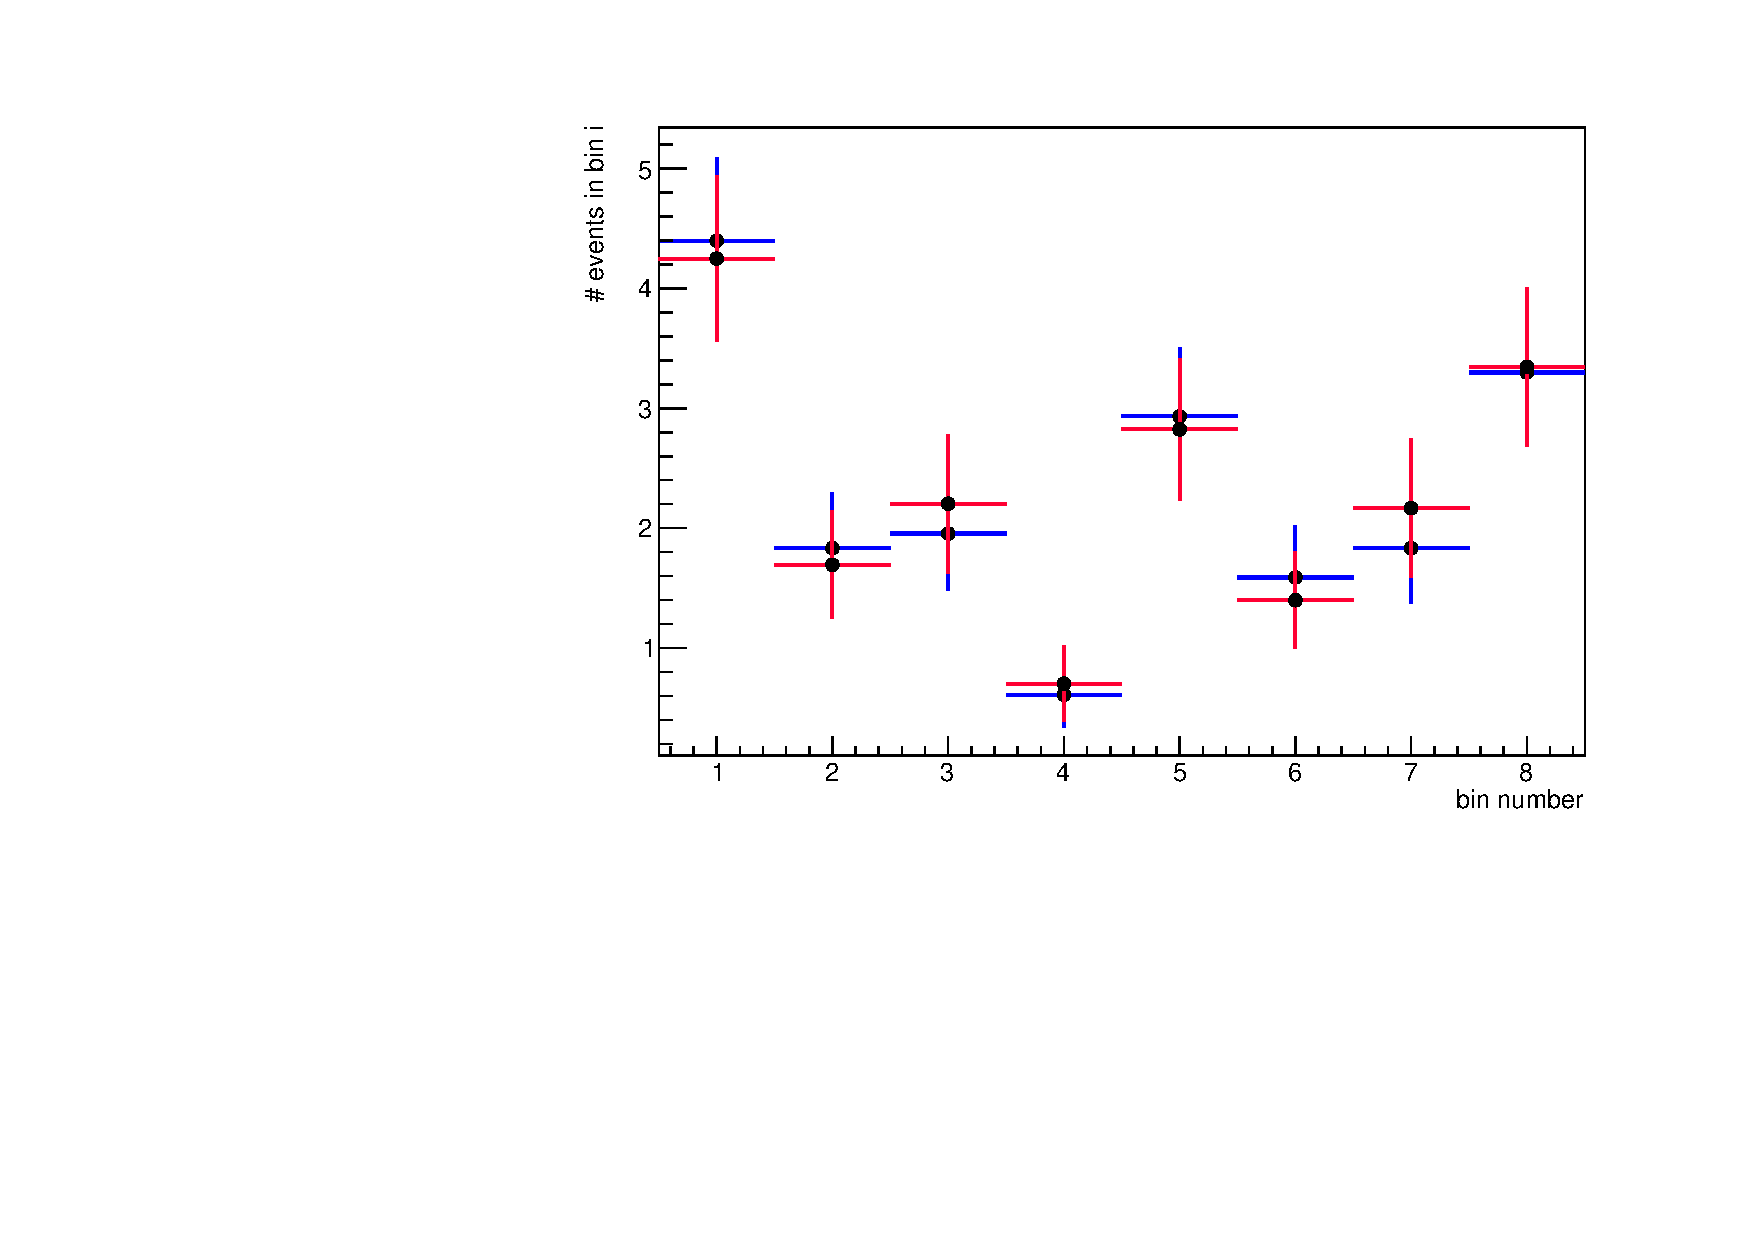
\includegraphics[width=1.\textwidth]{KsPiPi_selbias.pdf}
		\vspace*{-1.5cm}
	\end{center}
	\caption{\textit{Distribution of \KsPiPi vs \KsPiPi events over the bins determined by using \KsPiPi vs \KsPiPi MC. Blue: reversed \KS veto cut of FS>2, red: \KS veto cut of FS<0 as is used in the data sample.}}
	\label{fig:selbias}
\end{figure}
To compensate for this bias the values for the percentage of \KsPiPi vs \KsPiPi per bins obtained from the data are being weighted with the ratio of reversed \KS veto over the \KS veto efficiencies determined from the \KsPiPi vs \KsPiPi signal MC sample. This yields the total amount of \KsPiPi vs \KsPiPi contamination in the data sample listed below.
\begin{table}[!h]
	\begin{center}
		\begin{tabular}{c| l}
			bin i & $B^{peak}_i$  \\
			\hline 
			\hline
1 & 4.21854 $\pm$ 2 $\oplus$ 0.637882 \\ 
2 & 1.68165 $\pm$ 1.5 $\oplus$ 0.434214 \\ 
3 & 2.18858 $\pm$ 1.5 $\oplus$ 0.559566 \\ 
4 & 0.697849 $\pm$ 0.5 $\oplus$ 0.314724 \\ 
5 & 2.80305 $\pm$ 1.5 $\oplus$ 0.562877 \\ 
6 & 1.38776 $\pm$ 1.5 $\oplus$ 0.391982 \\ 
7 & 2.15081 $\pm$ 1.5 $\oplus$ 0.559324 \\ 
8 & 3.32175 $\pm$ 1.5 $\oplus$ 0.624964 \\
	\end{tabular}
	\end{center}
	\caption{\textit{Number of peaking background events per bin in the data sample. The first error is the Poisson error on the yields, the second error comes from the systematic uncertainty on the distribution over the bins.}}
	\vspace*{1cm}
\end{table}


\subsubsection{Cleanness of \KsPiPi vs \KsPiPi sample}
\label{sec:clean}
The gen MC suggest that the 'reversed \KS veto' yields a sample of 96\% \KsPiPi vs \KsPiPi events. The rest is distributed as follows:
\begin{itemize}
\item 2.8\% \4Pi vs \KsPiPi 
\item 0.2\% flat				
\item 1.0\% \KsPiPi vs \KsKs (with the \KsKs on the \KsPiPi side)
\end{itemize}
This will be accounted for in the systematic uncertainties in Section \ref{s:peakb}.\\

\section{Determination of number of flat background events}
\label{sec:flat}
The number of flat bkg events is determined using the usual sidebands (denoted A, B, C and D). The number of events in the sidebands is extrapolated to give the amount of flat bkg in the signal region using the equation
\begin{equation}
B_{tot}^{flat} = \frac{a_S}{a_D}N_D +  \sum_{j = A,B,C} \frac{a_S}{a_j} (N_j - \frac{a_j}{a_D}N_D)
\end{equation}
where $N_j$ is the number of events in sideband j, $a_j$ is the area of sideband j and $a_S$ is the area of the signal region. The results are listed below (no errors are assumed on the values of $a_j$).  
\begin{table}[!h]
	\begin{center}
		\begin{tabular}{c| c}
     $N_A$ & 1  \\
     $N_B$ & 0 \\
     $N_C$ & 20  \\
     $N_D$ & 2 \\
     \hline
     $B_{tot}^{flat}$  & 11.64  \\
    	\end{tabular}
	    \vspace*{-0.5cm}
    \end{center}
    \caption{\textit{Number of flat bkg in the sideband and extrapolated to the signal region.}}
\end{table}
  
To get the number of flat bkg events in bin i, the relative area of bin i is determined using the \texttt{dkpp\_babar.root} histogram. Assuming no error on the relative area of bin i the number of flat bkg events are:
\clearpage
\begin{table}[!h]
	\begin{center}
		\begin{tabular}{c| c}
			bins & number of flat bkg events \\
			\hline
1 & 3.85 $\pm$ 2 \\ 
2 & 1.33 $\pm$ 1 \\ 
3 & 0.74 $\pm$ 1 \\ 
4 & 0.69 $\pm$ 0.5 \\ 
5 & 1.55 $\pm$ 1.5 \\ 
6 & 0.94 $\pm$ 1 \\ 
7 & 0.98 $\pm$ 1 \\ 
8 & 1.56 $\pm$ 1.5 \\ 
	\end{tabular}
 \vspace*{-0.5cm}
\end{center}
\caption{\textit{Number of flat bkg events per bin.}}
\end{table} 

\section{Determination of the signal selection-efficiency}
The signal selection efficiency in each bin is determined using a sample of 266998 \KsPiPi vs \4Pi signal MC events.\\
%The signal selection efficiency in each bin is determined using a combination the efficiency of \KtPi vs \KsPiPi determined in an earlier analysis and \KsPiPi vs \4Pi signal MC. The signal MC is used to calculate the absolute selection efficiency while the efficiencies from \KtPi vs \KsPiPi are used to scale between the bins.\\
\begin{table}[!h]
	\begin{center}
		\begin{tabular}{c| l }
			bin & $\epsilon$  \\
			\hline
1 & 0.1553 $\pm$ 0.0012 \\ 
2 & 0.1529 $\pm$ 0.0021 \\ 
3 & 0.1761 $\pm$ 0.0029 \\ 
4 & 0.1671 $\pm$ 0.0030 \\ 
5 & 0.1583 $\pm$ 0.0019 \\ 
6 & 0.1642 $\pm$ 0.0025 \\ 
7 & 0.1551 $\pm$ 0.0024 \\ 
8 & 0.1607 $\pm$ 0.0020 \\
			\end{tabular}
	\end{center}
	\vspace*{-0.5cm}
	\caption{\textit{Signal efficiency per bin.}}
\end{table}

\clearpage
\section{Bkg substracted, efficiency corrected, rescaled signal yields}
\begin{table}[!h]
	\begin{center}
		\begin{tabular}{c| c }
			bin & $MM_i$  \\
			\hline
1 & 30.7804 $\pm$ 6.97383 $\oplus$ 0.241629 $\oplus$ 0.655893 \\ 
2 & 19.8284 $\pm$ 5.24652 $\oplus$ 0.26636 $\oplus$ 0.453361 \\ 
3 & 16.3846 $\pm$ 4.46561 $\oplus$ 0.273724 $\oplus$ 0.50743 \\ 
4 & 10.1474 $\pm$ 3.37991 $\oplus$ 0.180279 $\oplus$ 0.300871 \\ 
5 & 55.1394 $\pm$ 8.04054 $\oplus$ 0.676977 $\oplus$ 0.567952 \\ 
6 & 21.0775 $\pm$ 5.07712 $\oplus$ 0.325249 $\oplus$ 0.381242 \\ 
7 & 27.6736 $\pm$ 5.93899 $\oplus$ 0.432454 $\oplus$ 0.576076 \\ 
8 & 36.8818 $\pm$ 6.77579 $\oplus$ 0.448323 $\oplus$ 0.620996 \\ 
	\end{tabular}
\end{center}
\vspace*{-0.5cm}
\caption{\textit{$M_i$ + $M_{-i}$ The first error is the Poisson error on the raw data yields and the bkg yields, the second error comes from the limited data and MC samples used to determine the distribution of peaking bkg events and the third from the signal efficiency.}}
\label{tab:MMKs}
\end{table} 

\section{Summary}
\begin{table}[!h]
	\begin{center}
		\begin{tabular}{c| c | c | c|c}
		bin & raw yields & $B^{peak}_i$ & $B^{flat}_i$ &  signal  \\
		\hline 
		\hline
1 & 38 & 4.219 & 3.846 & 30.78 \\ 
2 & 22 & 1.682 & 1.327 & 19.83 \\ 
3 & 21 & 2.189 & 0.7433 & 16.38 \\ 
4 & 12 & 0.6978 & 0.6875 & 10.15 \\ 
5 & 59 & 2.803 & 1.55 & 55.14 \\ 
6 & 24 & 1.388 & 0.941 & 21.08 \\ 
7 & 30 & 2.151 & 0.9804 & 27.67 \\ 
8 & 42 & 3.322 & 1.561 & 36.88 \\ 
		\end{tabular}
	\end{center}
	\caption{\textit{Summary of contributions to the raw yields per bin.}}
\end{table}



%\chapter{The \lhcb experiment}
\chaptermark{Chapter3}
\label{chapter2}
%\addcontentsline{toc}{chapter}{The \lhcb experiment}
\lhcb is one of the four large experiments allocated at the Large Hadron Collider (\lhc). It is dedicated to the study of \CP violation and the search for new physics in rare decays of \B and \D mesons. As much focus is put on precision measurements of SM parameters as on the indirect detection of new physics that can intervene in loop and penguin diagrams.\\
The \lhc provides an ideal environment for new research in the sector of heavy flavour physics. The nominal center of mass energy of the \lhc was $\sqrt{s}=7\tev$ in 2011 and $\sqrt{s}=8\tev$ in 2012. The according \bbbar production cross sections at the hadron collider are $\sigma_{\bbbar}(7\tev)= 251.8\, \mu b$ and $\sigma_{\bbbar}(8\tev)= 291.6\, \mu b$ \cite{pythia} resulting in $6.5 \cdot 10^{11}$ \B hadrons produced in the \lhcb detector acceptance in both years combined ($3\invfb$ integrated luminosity collected in 2011 + 2012). 
Additionally to providing high statistics, the \lhc gives access to the system of the $B_s$ meson -- which was mostly beyond the reach of previous \bquark factories such as \babar and \belle \ -- allowing for the investigation of \CP violation and the search for new physics in the \Bs system.\\ 
The \lhcb collaboration has already published several new results constraining SM parameters and possible contributions from new physics, for example the restraining of SUSY parameters with the decays $B^0_s \rightarrow \mup \mun$ and $B^0 \rightarrow \mup \mun$ \cite{bsmumu}.\\
\\
This chapter is dedicated to the description of the \lhcb detector. After a general overview over the detector the different subdetectors of the tracking system and the particle identification system are presented and a summary of the detector performance is given. Then the \lhcb trigger system and different trigger lines are introduced. At the end of this chapter \lhcb software is introduced. \\
 
\section{The \lhcb detector}
\label{sec:lhcb}
The \lhcb detector was designed as a single arm forward spectrometer \cite{lhcbletter} to match the kinematics of \bbbar production shown in Figure \ref{fig:pseudorapidity}. Corresponding to this distribution, the \lhcb detector covers an angular range of $10\,$mrad$\, - \, 300 \,$mrad in the bending and $10\,$mrad$\, - \, 250 \,$mrad in the non-bending plane. Both for $7\tev$ and $8\tev$ $25\,\%$ of the produced \bbbar pairs are in the detector acceptance.\\
\\
To enable precision measurements, the \lhcb detector was build with a minimal amount of material budget. Additionally, the \lhc conducts luminosity levelling for \lhcb. The proton-beams are tuned to be displaced with respect to each other at the \lhcb collision point, giving the bunches only a small overlap while colliding. The luminosity levelling is performed in a manner that keeps the number of proton-proton interaction per bunch-crossing adjusted to an average of $1.5$ throughout the entire run.\\
\\
The \lhcb detector is composed of several subdetectors shown in Figure \ref{fig:lhcb} and presented in the following sections.
Altogether the \lhcb detector incorporates precision vertexting and tracking, worldwide leading particle identification and efficient triggering through a system of dynamic triggers.
 \begin{figure}[ht]
  \begin{center}
  \subfigure{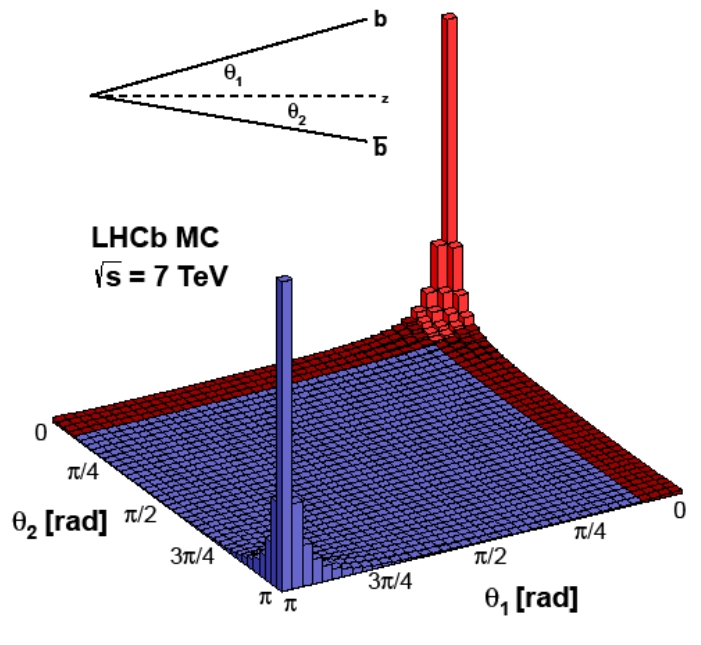
\includegraphics[width=0.4\textwidth]{pseudorapidity.jpg}}
    \subfigure{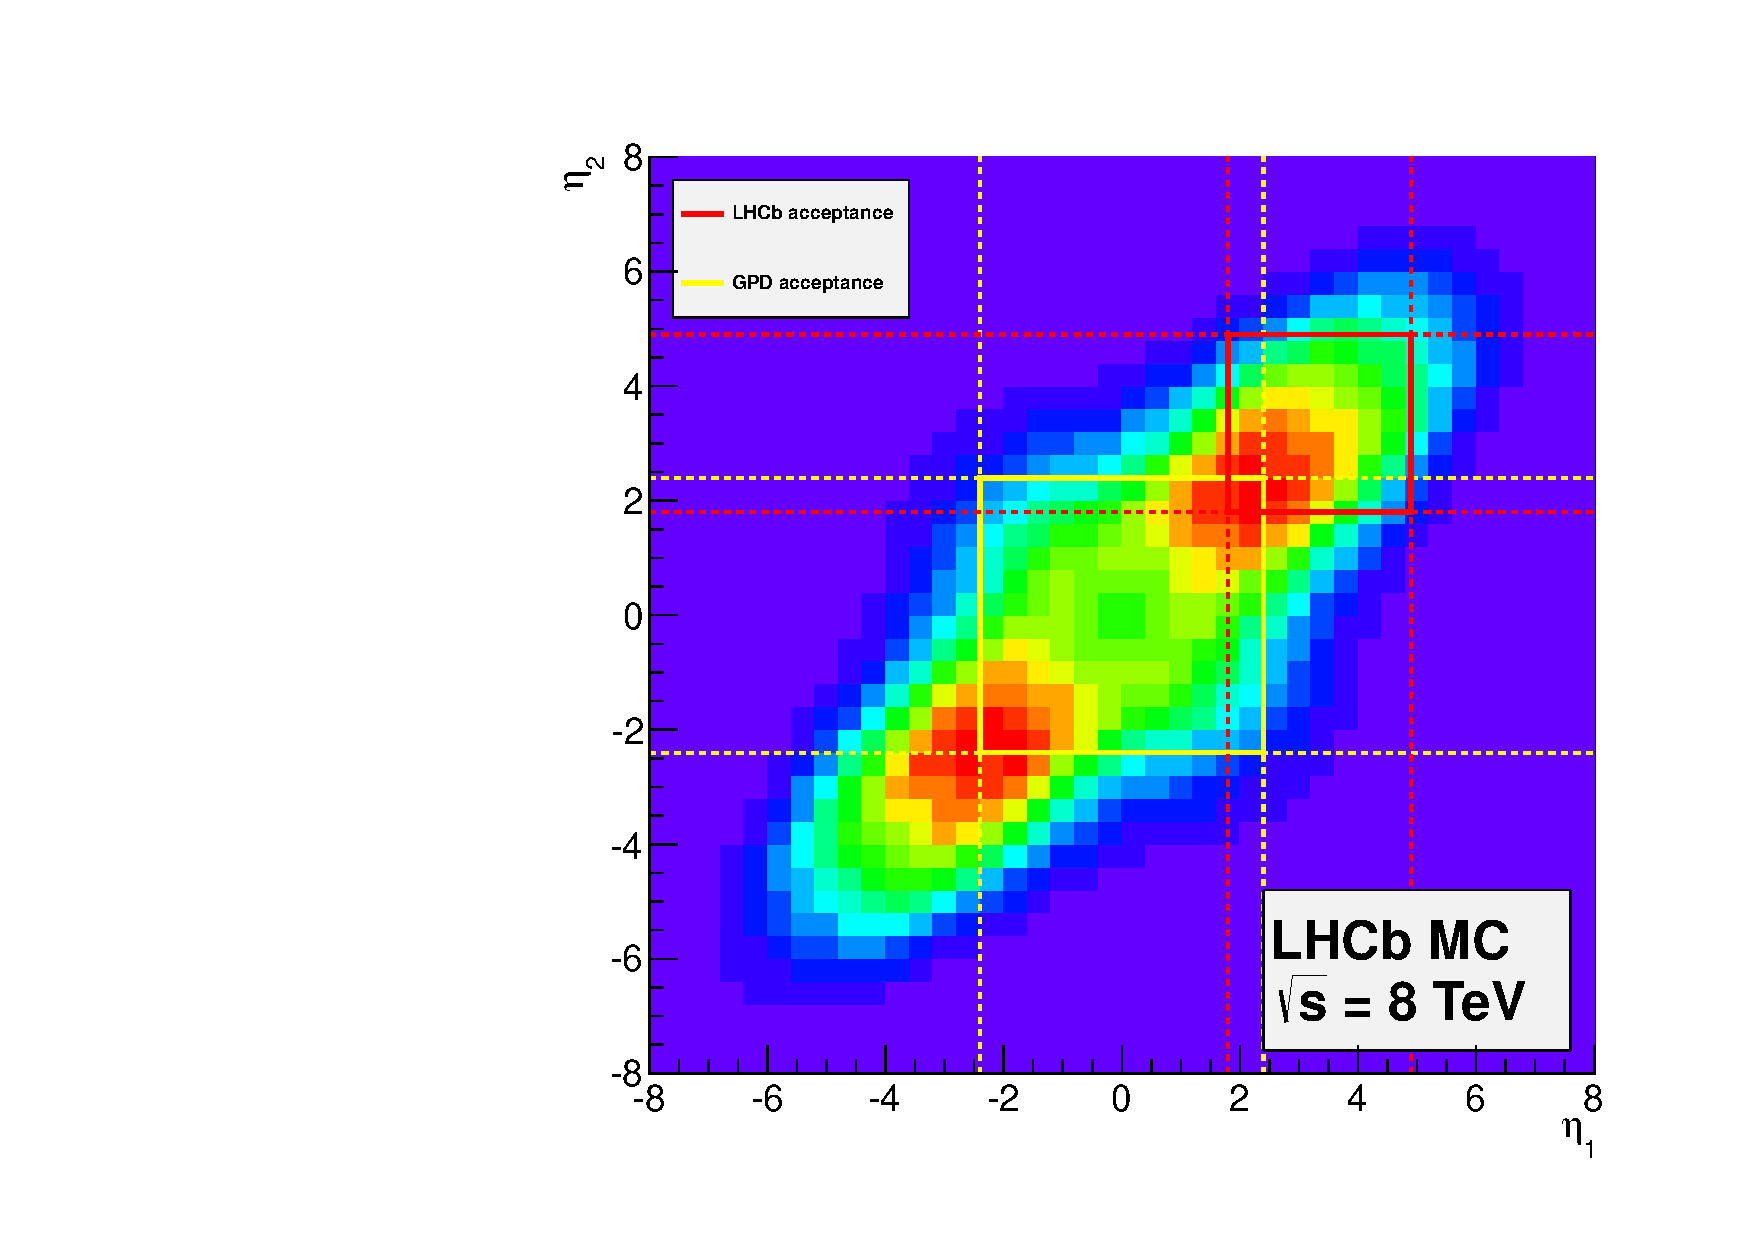
\includegraphics[width=0.42\textwidth]{acceptance.pdf}}
  \vspace*{-0.5cm}
  \end{center}
  \caption{\textit{Angular distribution of \bbbar produced in proton-proton collisions. At hadron colliders the dominant mechanism for \bbbar production is through gluon gluon fusion. Due to the statistical partition of the energy inside the protons the \bbbar pairs originated from the gluon gluon interactions are boosted in the forward or backward direction.}\cite{pythia}}
  \label{fig:pseudorapidity}
\end{figure}
\newpage

\noindent%
\begin{minipage}{\linewidth}
\makebox[\linewidth]{%
  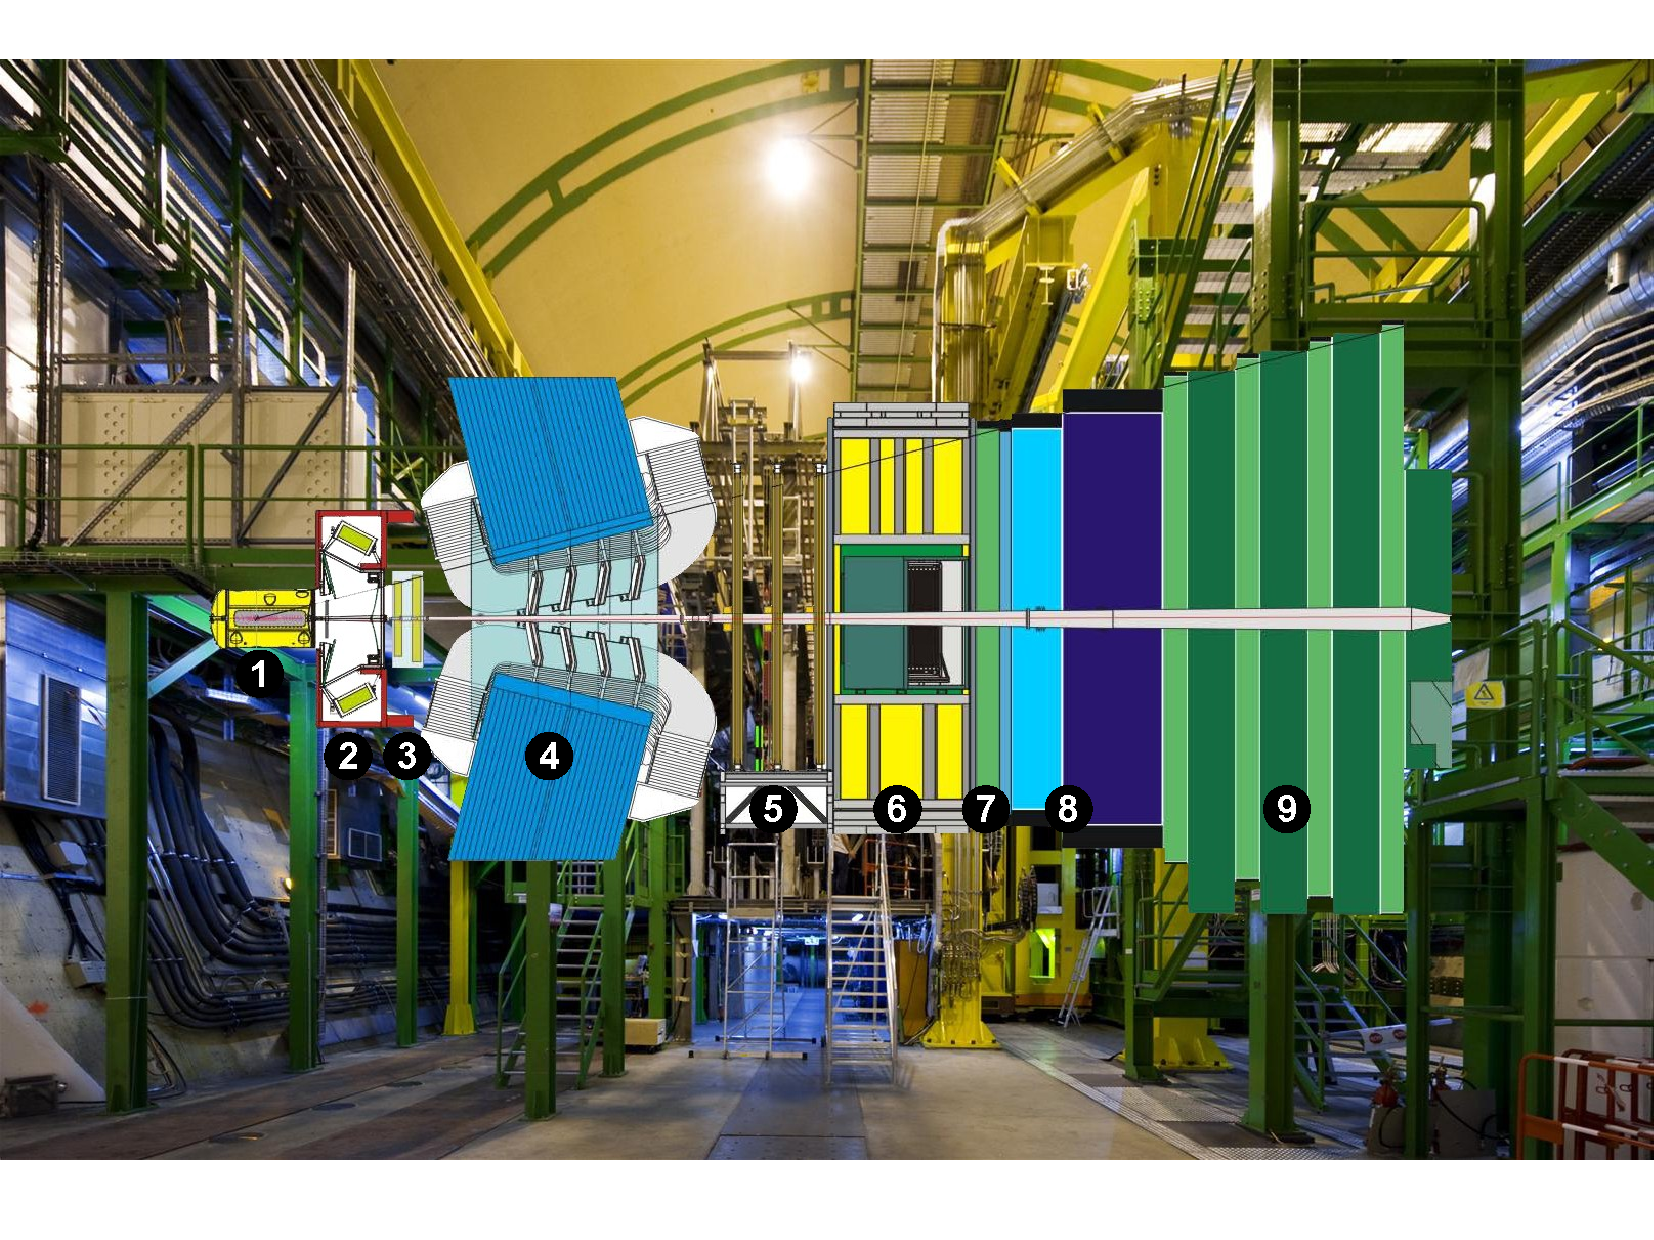
\includegraphics[angle=90, width=0.95\textwidth]{lhcb.pdf}}
\captionof{figure}{\textit{The \lhcb detector. 1: Vertex Locator (\velo), 2: Ring Imaging Cherenkov detector 1 (\richone), 3: Tracker Turicensis (\ttracker), 4: the magnet, 5: the tracking stations, 6: Ring Imaging Cherenkov detector 2 (\richtwo), 7: Muon chamber 1 (\Mone), 8: Scintillating Pad Detector (\spd), PreShower Detector (\presh), electromagnetic calorimeter (\ecal) and hadronic calorimeter (\hcal), 9: Muon chambers 2 to 5 (\Mtwo to \Mfive).}\cite{lhcb}}
  \label{fig:lhcb}
\end{minipage}
\newpage

\subsection{The tracking system}
The \lhcb tracking system's purpose is the detection of charged particle tracks and the measurement of their momenta. It is also responsible for the reconstruction of production and decay vertices of \B and \D mesons. This is essential not only for lifetime measurements but also for an efficient background rejection in the analysis of rare decays.\\
The tracking system consists of the Vertex Locator (\velo), the magnet, the Silicon Tracker (\st) and the Outer Tracker (\ot). The Silicon Tracker makes up for the entire Tracker Turicensis (\ttracker) and the Inner Tracker (\intr) which is the inner part of the three tracking stations (\Tone, \Ttwo and \Tthree) downstream of the magnet. The Outer Tracker is the outer part of the tracking stations (see 5. in Figure \ref{fig:lhcb}).
\\
%% Measure the momentum of charged particles

\subsubsection{The Vertex Locator (\velo)}
The \velo \cite{velo} accurately measures the positions of tracks close to the interaction point and allows for a very precise reconstruction of the primary vertex and the impact parameters of all tracks.\\
As shown in Figure \ref{fig:velo}, the vertex locator is approximately $1 \m$ long and consists of 21 disc-like modules arranged around the beam pipe. Each module is composed of two halfs, each having two sides with silicon strips arranged to measure the $R$ and $\Phi$ coordinate respectively. The modules can be approached as close as $8\mm$ to the beam and have a total radius of $4.2 \cm$. The strip pitch varies from $38 \mum $ wide strips nearest to the beam pipe to $102 \mum$ wide strips for the $R$ sensors and $79 \mum$ wide strips for the $\Phi$ sensors at the outer margin according to the particle density in the detector.\\
\begin{figure}[h]
  \begin{center}
  	\vspace*{-0.8cm}
    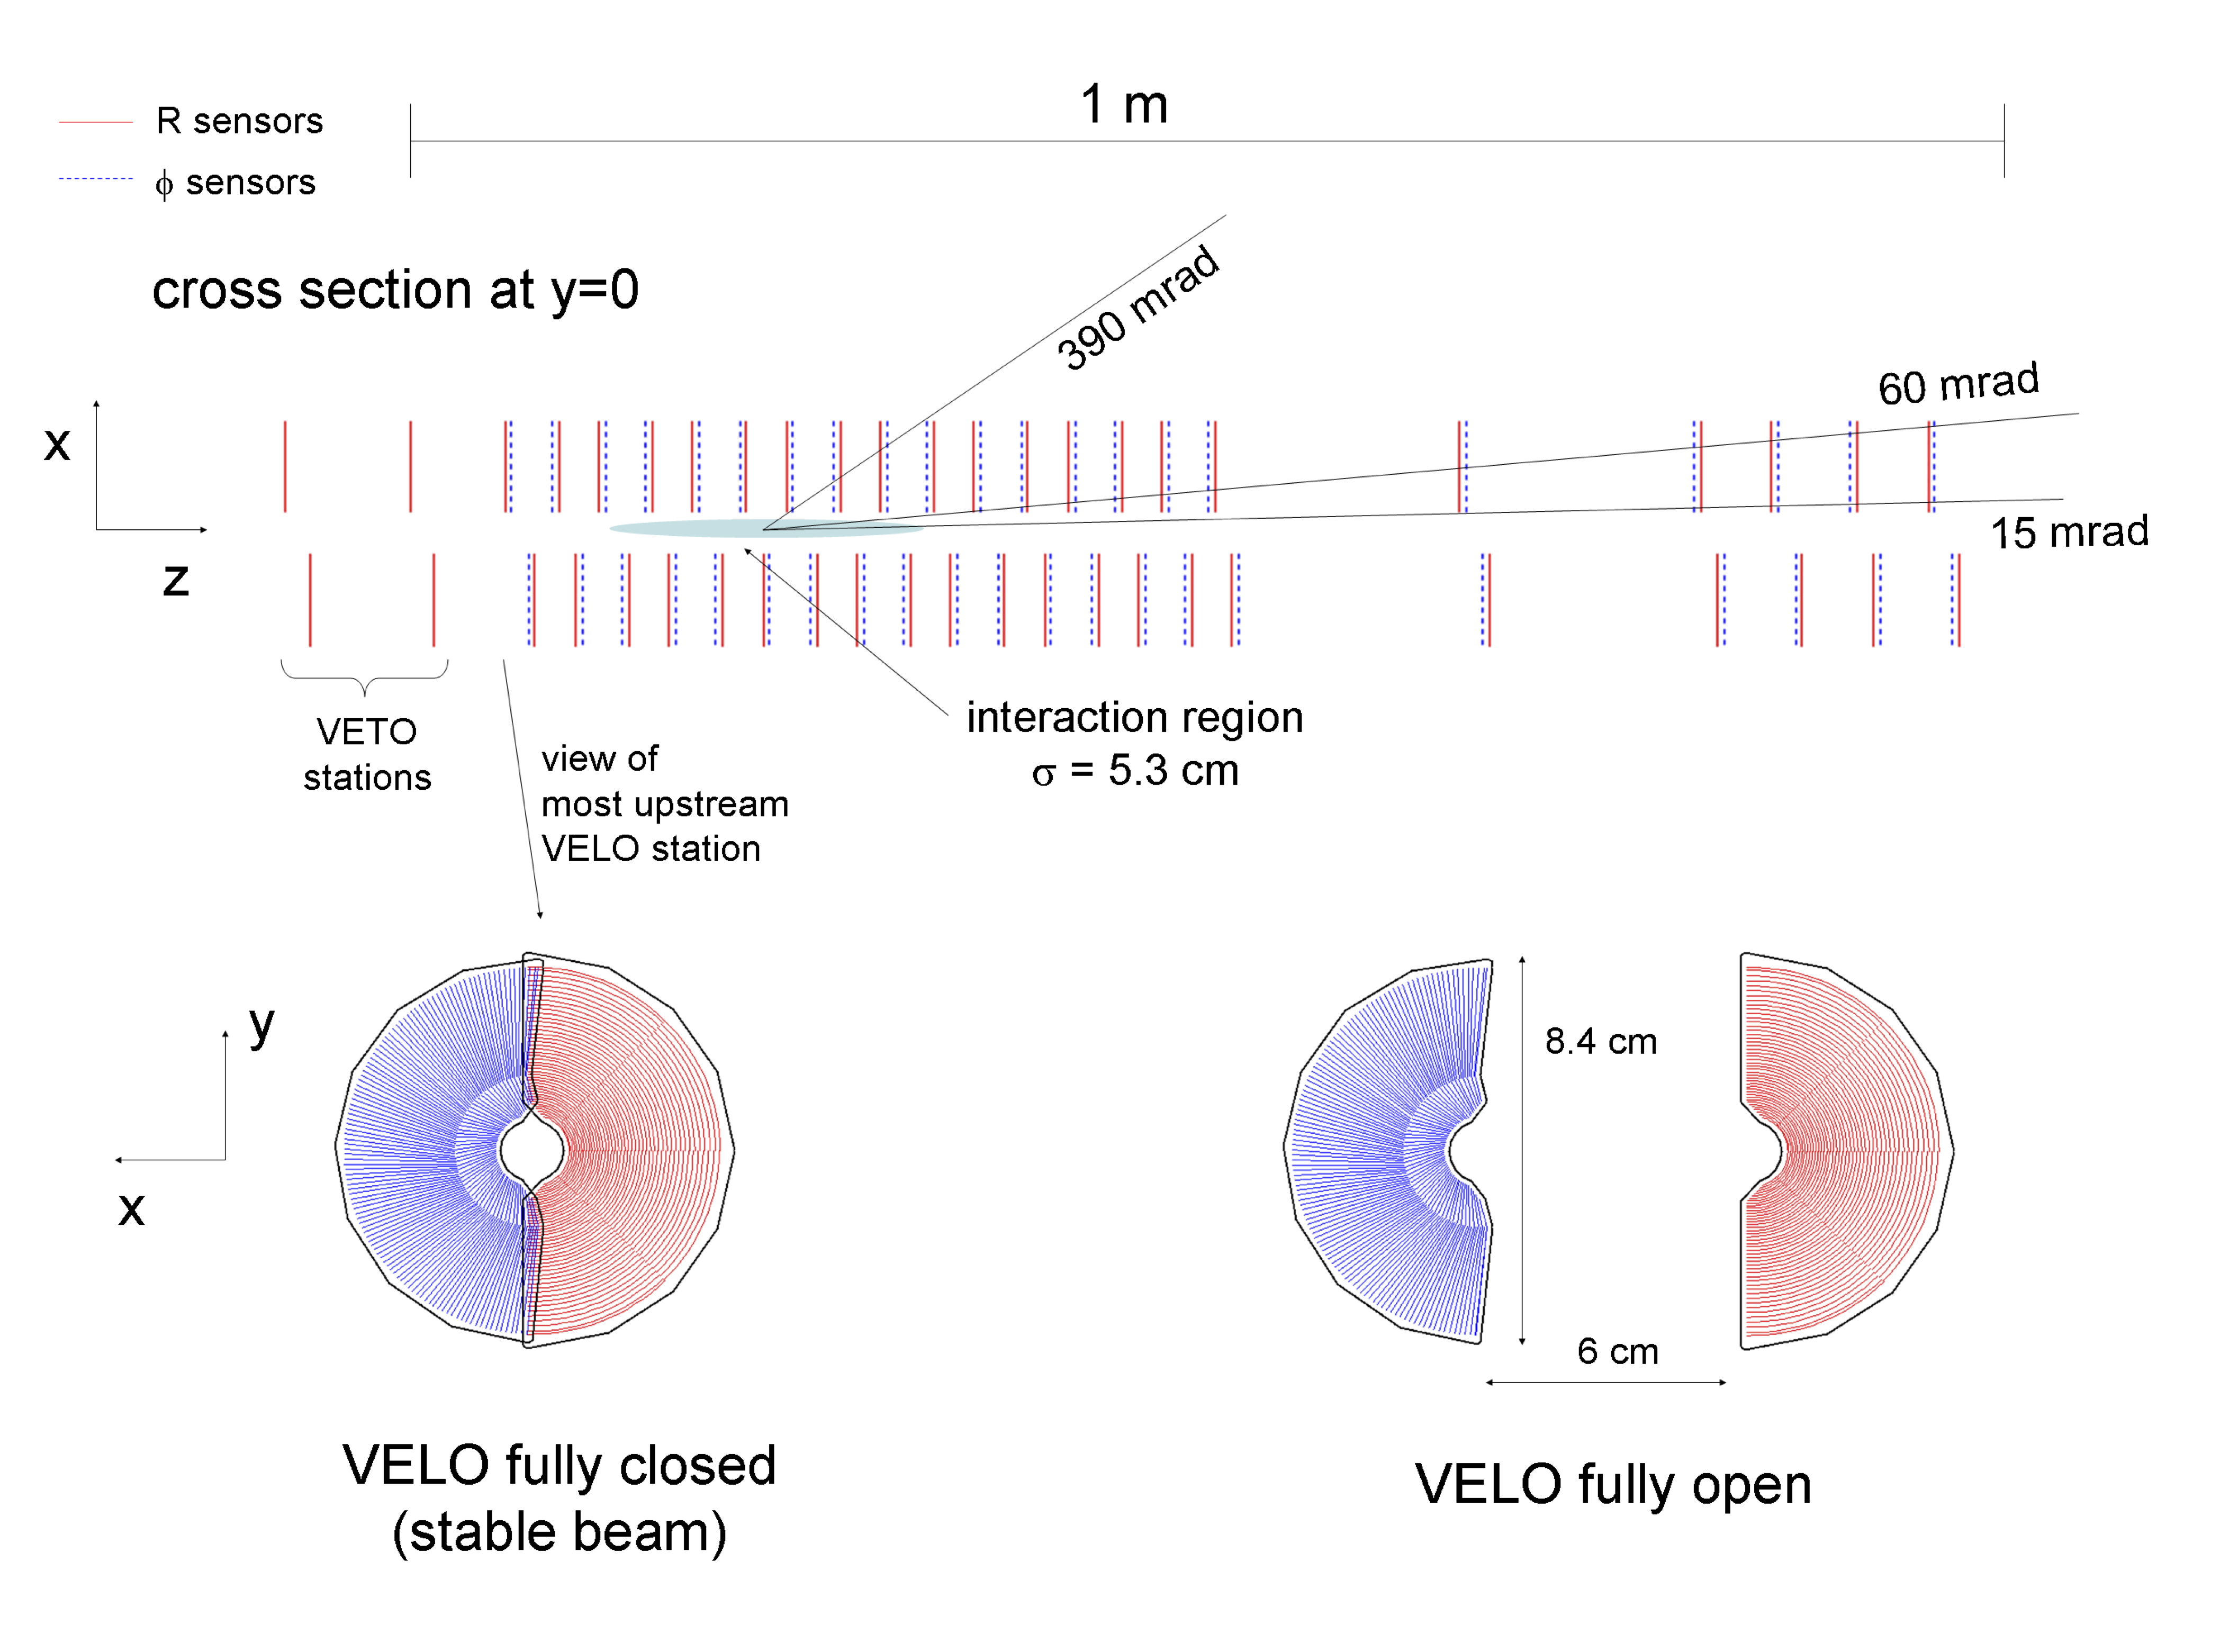
\includegraphics[width=0.75\textwidth]{velo.png}
  \vspace*{-1.0cm}
  \end{center}
  \caption{\textit{Schematic illustration of the \velo. Top: top view of the 21 modules. Bottom: Two \velo modules shown with both halfs to measure $\Phi$ (blue) and $R$ (red). Module in closed position (left) and in open position (right) which is engaged while unstable beam conditions.}\cite{velo}}
  \label{fig:velo}
\end{figure}


\subsubsection{The magnet}
The \lhcb magnet \cite{magnet} is a warm dipole magnet with saddle shaped coils. The streamlines of the magnetic field are parallel to the $y$ axis, making the $(x-z)$ plane the bending plane. Since the relative momentum resolution varies with 
\begin{equation}
\frac{\sigma_p}{p} \propto \frac{1}{B}
\end{equation}
the integrated magnetic field was chosen to be $4\, $Tm. Additionally, the magnet polarisation is regularly changed to reduce systematic effects on measurements due to geometrical acceptances.

\subsubsection{The Silicon Tracker (\st)}
The \st \cite{it} implements silicon microstrip technology for the Tracker Turicensis (\ttracker) and the Inner Tracker (\intr) with a strip pitch of about $200 \mum$. Combining the \ttracker and the \intr, the \st has four stations. Each of this four stations consists of four layers that are arranged in a $(x-u-v-x)$ geometry with vertical strips in the $x$ layers and strips rotated by a stereo angle of $-5^{\circ}$ and $+5^{\circ}$ in the $u$ and $v$ layer respectively.\\
The \ttracker is located upstream of the magnet and allows reconstruction of low momentum particles which are swept out of the detector acceptance after entering the magnetic field. It also provides information for the trigger by performing transverse momentum measurements for tracks with a large impact parameter.
With an area of $140 \cm$ width and $120 \cm$ height, the \ttracker covers the total \lhcb angular acceptance. As can be seen in Figure \ref{fig:st}, the layers of the \ttracker are divided into three different types of sectors ($K$, $M$ and $L$). According to the particle flux that is highest close to the beam pipe and drops of radially, the length of the silicon strips increases from the innermost to the outermost sensors.\\
The \intr covers the inner region of the tracking stations where the particle flux is highest. One layer of the \intr can be seen in Figure \ref{fig:st} on the right. It consists of four pieces arranged in a criss-cross pattern around the beam pipe that cover a total area of $0.35 \m^2$. 
%Each piece contains seven detector modules made out of one or two silicon sensors. The silicon sensors each carry about $400$ silicon microstrips.
\begin{figure}[ht]
  \begin{center}
  \vspace*{-0.cm}
  \subfigure{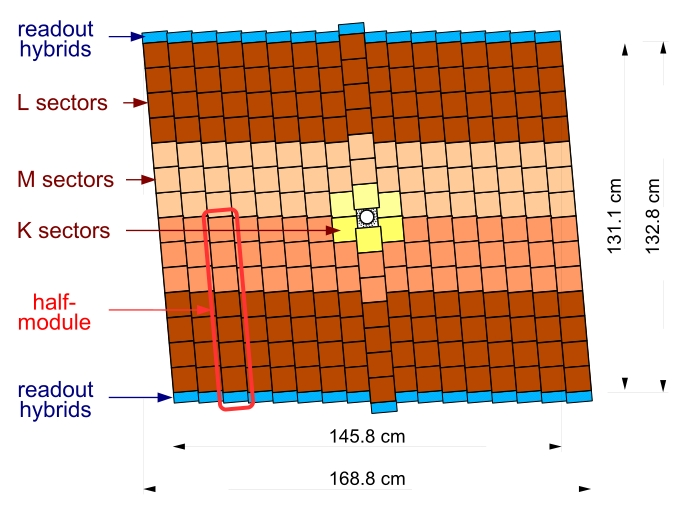
\includegraphics[width=0.49\textwidth]{tt.jpg}}
    \subfigure{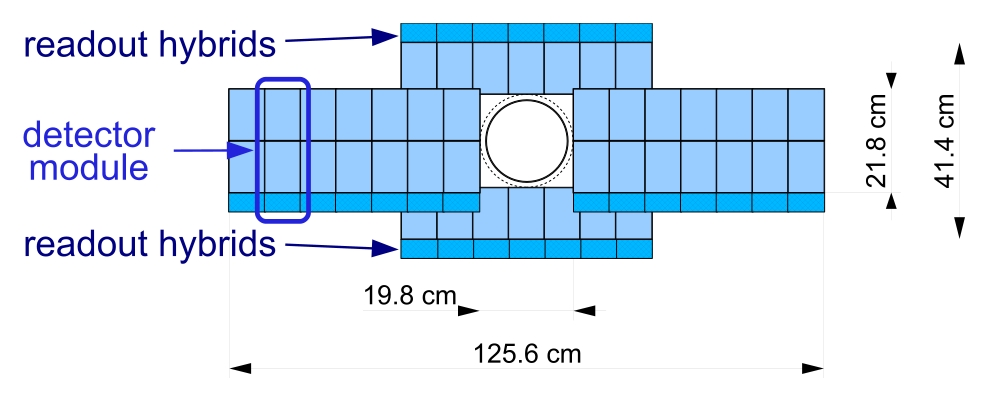
\includegraphics[width=0.49\textwidth]{it.jpg}\vspace{5cm}}
  \vspace*{-1.0cm}
  \end{center}
  \caption{\textit{The two parts of the Silicon Tracker (\st). The Tracker Turicensis (\ttracker) with the three different types of modules (left) and the Inner Tracker (\intr) which is part of the tracking stations (right).}\cite{it}}
  \label{fig:st}
\end{figure}



\subsubsection{The Outer Tracker (\ot)}
The \ot \cite{ot} covers the outer region of the tracking stations. Since the particle flux is lower in this area the \ot implements the technology of drift tubes.
As for the \st, each \ot tracking station has four layers arranged in a $(x-u-v-x)$ geometry with vertical strips in the $x$ layers and strips rotated by a stereo angle of $-5^{\circ}$ and $+5^{\circ}$ in the $u$ and $v$ layer respectively. Each layer covers the total \lhcb angular acceptance. The inner boundaries filled by the \intr were determined by the requirement that occupancies in the straw-tubes should not exceed $10\%$ at the nominal running luminosity of $2\cdot 10^{32} \cm^{-2}s^{-1}$.\\
The structure of the \ot layers is shown in Figure \ref{fig:ot}. Each layer is  build of two different types of modules. All modules are composed of two staggered layers (monolay-
\begin{figure}[ht]
  \begin{center}
  	\vspace*{-0.5cm}
    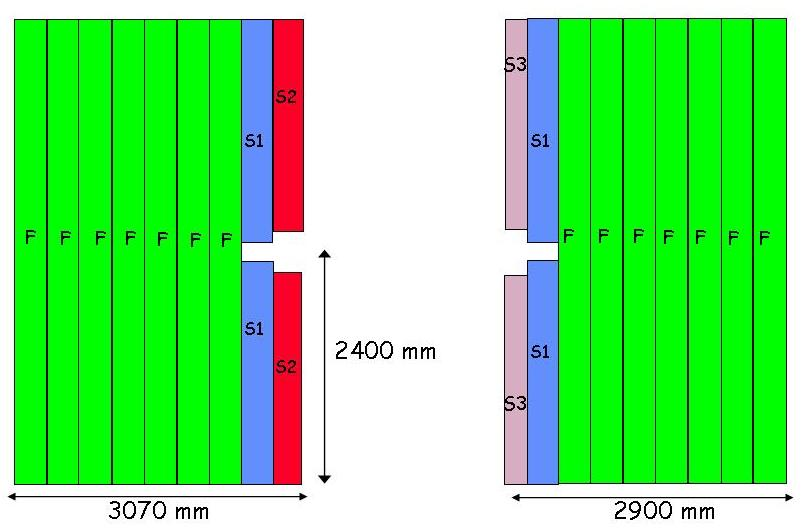
\includegraphics[width=0.45\textwidth]{OT-Modules.jpg}
  \vspace*{-0.5cm}
  \end{center}
  \caption{\textit{One layer of the Outer Tracker (\ot) with the long $F$ modules and the shorter $S$ modules combined out of $256$ and $128$ drift tubes respectively.}\cite{ot}}
  \label{fig:ot}
\end{figure}
ers) of straw-tubes.
The $F$ modules are $4.85\m$ long and consist of $256$ straw-tubes. Their monolayers are split along the $y$ axis, at different positions for each monolayer to avoid insensitive regions in the middle of the modules.
The $S$ modules are shorter than the $F$ modules and located above and below the beam pipe. Each of the $S$ modules has $128$ straw-tubes.\\
All straw-tubes are $5 \mm$ thick and filled with a gas mixture of $Argon$ and $CO_2$ ($70:30$) which combines fast response time ($<50 \ns$) with a high resolution of the drift coordinate ($200\mum$).\\


%\subsubsection{Performance}
%The \lhcb tracking system has an average relative momentum resolution of $0.5 \%$. \\
%The resolution of the $x$ and $y$ coordinates of the primary vertex and the resolution on the impact parameter's $x$ coordinate are shown in Figure \ref{fig:resolution}. For 25 tracks a resolution of $13 \mum$ on the $x$ and $y$ coordinates and a resolution of $69 \mum$ on the $z$ coordinate of the primary vertex can be reached. Additionally and equally excellent impact parameter resolution of $<35 \mum$ for tracks with a transverse momentum $p_T>1 \gev$ can be obtained.
%\begin{figure}[ht]
%  \begin{center}
%  \subfigure{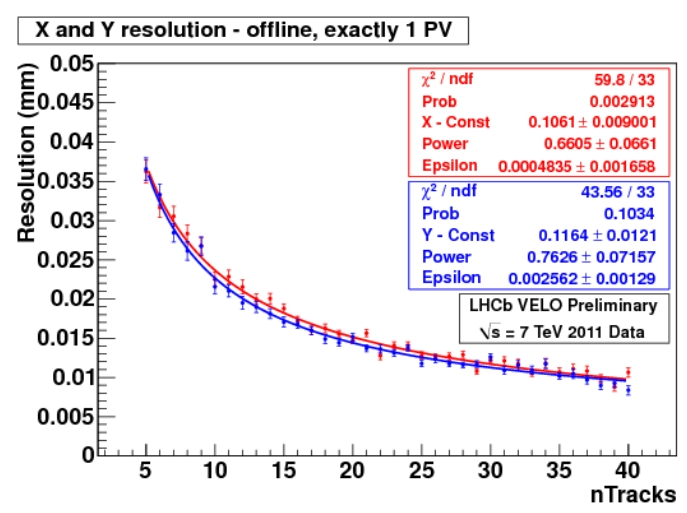
\includegraphics[width=0.45\textwidth]{PVresolution.jpg}}
%    \subfigure{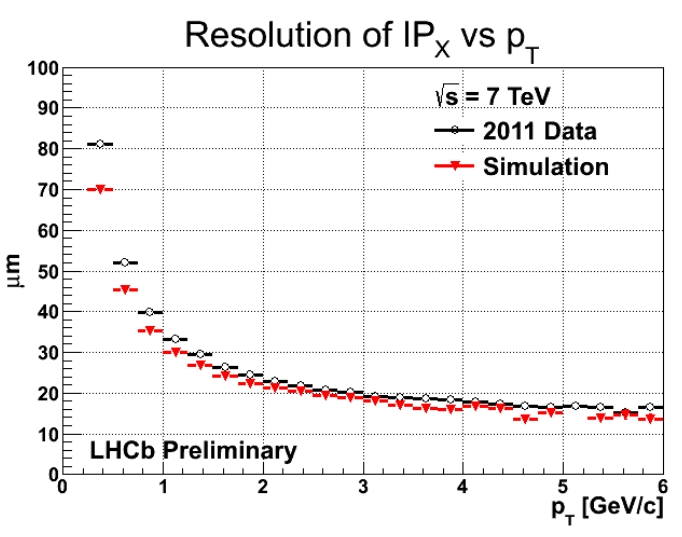
\includegraphics[width=0.45\textwidth]{IPresolution.jpg}}
%  \vspace*{-1.0cm}
%  \end{center}
%  \caption{\textit{Summary of the performance of \lhcb tracking system obtained from 2011 data and Monte Carlo. The primary vertex resolution for the $x$ and $y$ coordinates as a function of the number of tracks (left) and the of the $x$ coordinate of the impact parameter as a function of the transverse momentum $p_T$.}}
%  \label{fig:resolution}
%\end{figure}

\subsection{The particle identification system}
The \lhcb particle identification system consists of two Ring Imaging CHerenkov (\rich) detectors, the calorimeter system and the muon system. The information of these subdetectors is combined later in the offline analysis and evaluated with the use of a likelihood function.\\

\subsubsection{The \richone and \richtwo}
The \lhcb detector includes two RICHs \cite{rich} to allow for a precise separation of charged pions and kaons over the entire momentum spectrum. The separation follows through analysis of the Cherenkov light emitted by ultra-relativistic charged particles when traversing the gas of the RICHs \cite{WRLeo}.\\
\richone is placed between the \velo and the \ttracker and covers the full angular acceptance of the \lhcb detector. It uses a mixture of aerogel and $C_4F_{10}$ radiators to distinguish charged particles with a momentum between $1 \gevc \, - \, 60\gevc$.\\
\richtwo is located downstream of the magnet behind the tracking stations. It is designed to cover the momentum range from $15\gevc$ to $100\gevc$ using $CF_4$ radiator gas. Corresponding to the region where high momentum particles are produced, the \richtwo covers an angular acceptance of $15\,$mrad to $120\,$mrad (bending plane) and $100\,$mrad (non-bending plane).\\
The Cherenkov angle depending on the particles momentum is plotted in Figure \ref{fig:richrad} for different particles in the \rich radiators.
\begin{figure}[ht]
  \begin{center}
  	\vspace*{-0.5cm}
    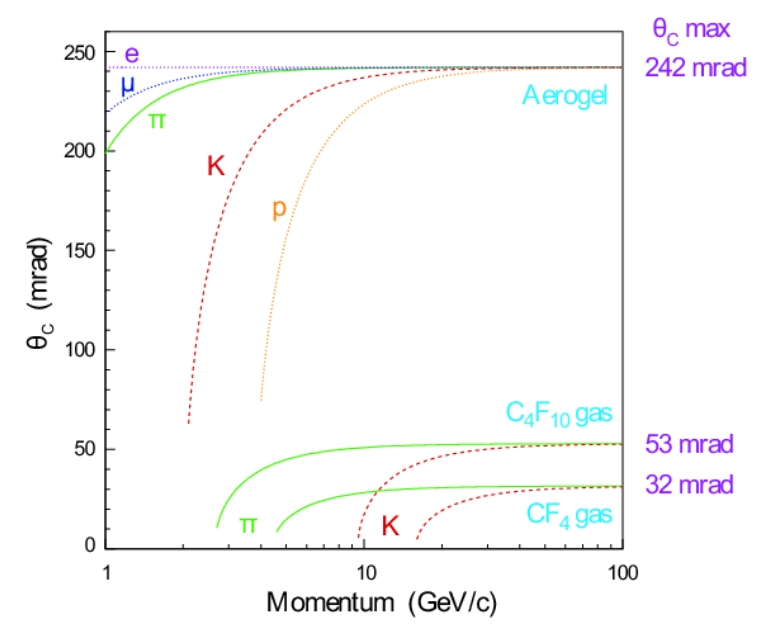
\includegraphics[width=0.55\textwidth]{richrad.jpg}
  \vspace*{-0.8cm}
  \end{center}
  \caption{\textit{Cherenkov angle versus the particle momentum for different particles in the \rich radiators.}\cite{rich}}
  \label{fig:richrad}
  \vspace*{-0.5cm}
\end{figure}

\subsubsection{The calorimeter system}
The \lhcb calorimeter system \cite{calo} consists of a Preshower detector (\presh), a Scintillating Pad Detector (\spd), an electromagnetic calorimeter (\ecal) and a hadronic calorimeter (\hcal). The main purpose of the calorimeter system is the identification of light particles such as electrons and neutral particles such as photons or \piz as illustrated in Figure \ref{fig:pid} \cite{pidcalo} and the measurement of energy and position of neutral particles that can't be detected by the tracking system. The calorimeters also provide information for the hardware based \lone trigger (see Section \ref{sec:l0}).
\begin{figure}[ht]
\vspace{-0.3cm}
  \begin{center}
    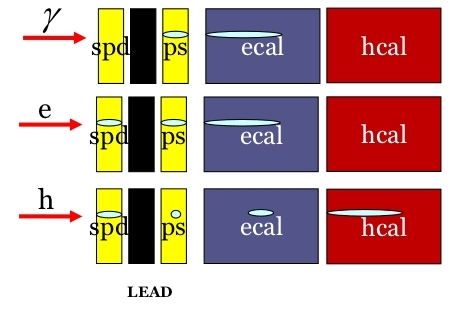
\includegraphics[width=0.5\textwidth]{CAL.jpg}
  \end{center}
  \vspace*{-1cm}
  \caption{\textit{Schematic illustration of the particle separation using the calorimeter system. The lead layer between the Scintillation Pad Detector (\spd) and the PreShower detector (\presh) is thick enough to induce electromagnetic showers.}\cite{calo}}
  \label{fig:pid}
  \vspace*{-0.5cm}
\end{figure}
% but too thin to start a significant hadronic shower

Each subdetector of the calorimeter system is composed of square cells varying in size according to the particle flux. For the \spd, \presh and the \ecal three different zones were chosen with cell sizes of $4\cm$, $6\cm$ and $12\cm$ as shown in Figure \ref{fig:calo}. The \hcal is segmented into two zones with larger cells ($13.13\cm$ in the inner section and $26.26\cm$ in the outer section) because of the size of hadronic showers. All calorimeters implement the technology of scintillation light that is transmitted to Photo-Multipliers (PMT) by wavelength-shifting (WLS) fibres.\\
\begin{figure}[ht]
  \begin{center}
  	\vspace*{-0.8cm}
    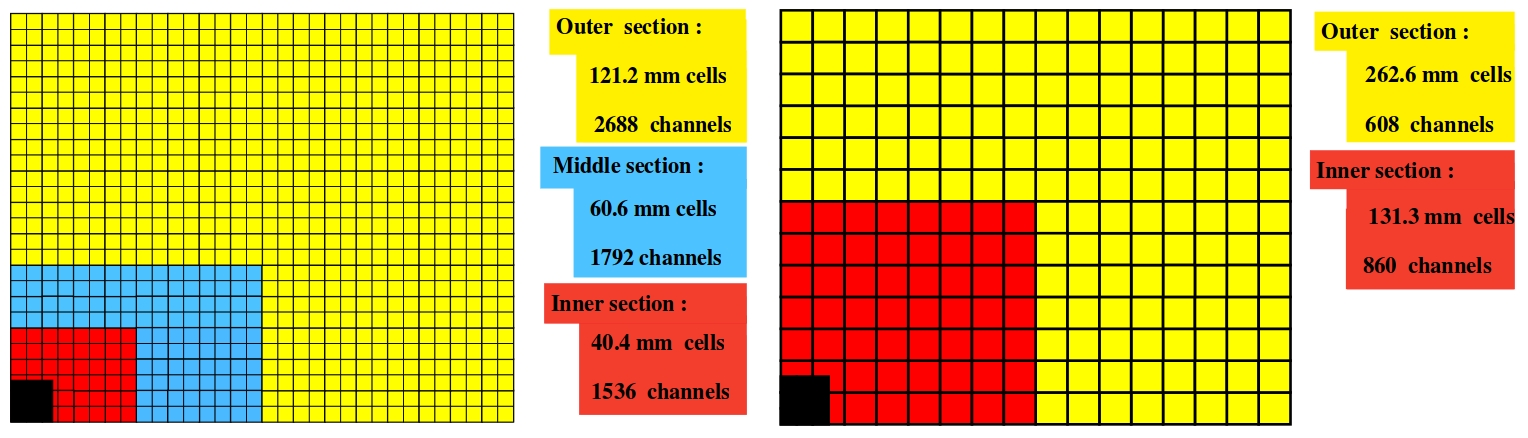
\includegraphics[width=0.85\textwidth]{calocells.jpg}
  \vspace*{-0.5cm}
  \end{center}
  \caption{\textit{Schematic illustration of the segmentation of the Scintillating Pad Detector (\spd), PreShower detector (\presh) and the \ecal (left) and the \hcal (right). The pictures show one quarter of the calorimeter surfaces. The black area on the bottom left of both images is the area close to the beam pipe where the particle flux is too high for any calorimeter performance.}\cite{calo}}
  \label{fig:calo}
  \vspace*{-0.5cm}
\end{figure}

The \presh and the \spd are located before the \ecal and separated by lead sheet of $2.5 \, \Xrad$ thickness allowing for a separation of electrons from a high background of pions. Both \presh and \spd are made of one single layer of $15\mm$ thick plastic-scintillator tiles.\\
The \ecal is composed of cells that are build after the shashlik  principle, one cell is composed of alternating layers of $2\mm$ thick lead and $4\mm$ thick polystyrene scintillator tiles. One cell, made out of 66 lead and scintillator layers, is illustrated in Figure \ref{fig:calos}.
The \hcal employs a non-typical structure where the scintillating tiles are arranged parallel to the beam pipe as shown in Figure \ref{fig:calos}. The absorber for the \hcal was chosen to be $1\cm$ iron tiles and the scintillator layers are made out of $3\mm$ thick doped polystyrene tiles.
\begin{figure}[ht]
  \vspace*{-0.5cm}
  \begin{center}
  \subfigure{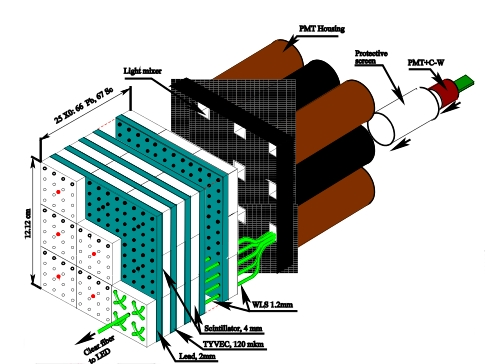
\includegraphics[width=0.45\textwidth]{ECAL.jpg}}
   \subfigure{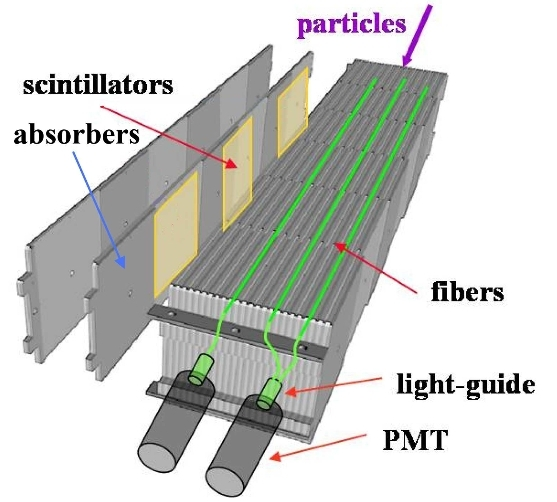
\includegraphics[width=0.43\textwidth]{hcal1.jpg}}
  \vspace*{-0.8cm}
  \end{center}
  \caption{\textit{One cell of the \ecal (left) and the \hcal (right). The scintillating tiles of the \ecal are arranged perpendicular to the beam while they are parallel to the beam for the \hcal. The absorber is made of lead for the \ecal and iron for the \hcal.}\cite{calo}}
  \label{fig:calos}
\end{figure}


\subsubsection{The muon chambers}
The \lhcb detector contains five muon stations (\Mone - \Mfive) dedicated to muon identification and muon triggering \cite{muon}.\\
The first muon station \Mone is placed upstream of the calorimeters to provide a precise transverse momentum measurement. The other muon stations are placed downstream of the calorimeters and interleaved with $80\cm$ thick iron absorbers. The stations \Mtwo and \Mthree yield a very good spacial resolution for the tracks while the last two stations only deliver information for the particle identification. The side view of the muon system is shown in Figure \ref{fig:muons}.\\
As can be seen on the left in Figure \ref{fig:muons}, each muon chamber is divided into four regions R1 to R4. The granularity in the regions decreases radially which provides an isotropic channel occupancy for each muon station. Except for the inner region R1 of \Mone, all muon stations are composed of Multi Wire Proportional Chambers (MWPC). R1 of \Mone implements the Triple GEM \cite{gem} technology because the particle flux in this region would overburden the MWPC.\\
\begin{figure}[ht]
\vspace*{-0.5cm}
  \begin{center}
  \subfigure{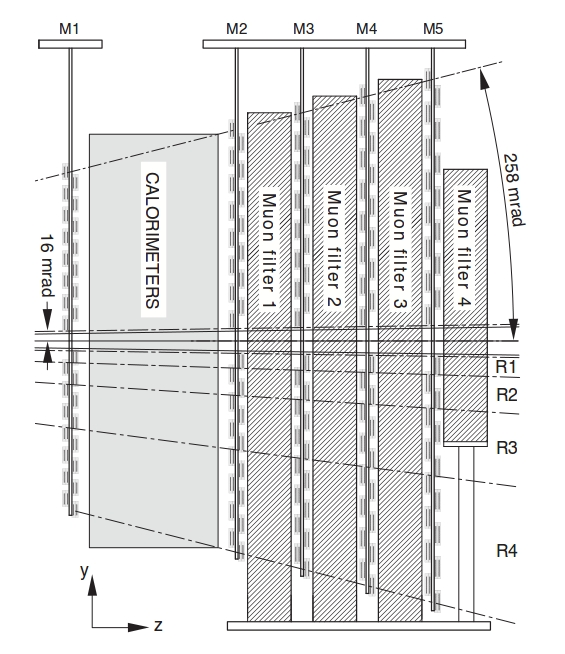
\includegraphics[width=0.35\textwidth]{muon2.jpg}}
   \subfigure{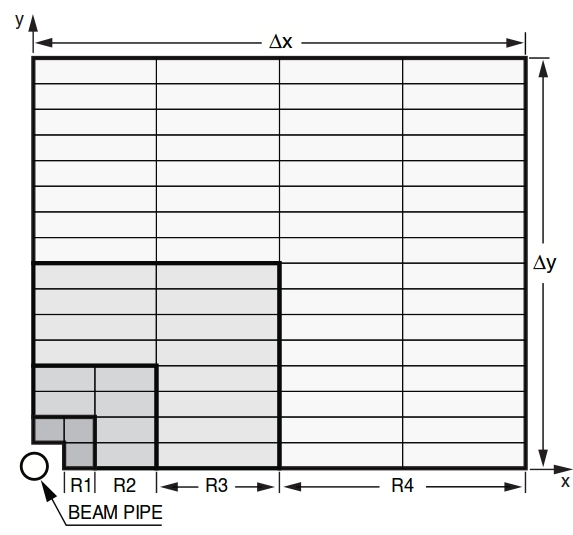
\includegraphics[width=0.35\textwidth]{muon1.jpg}}
  \vspace*{-1.0cm}
  \end{center}
  \caption{\textit{Side view of the muon stations (left) and the schematic front view of the upper right quarter of one muon station with the segmentation into four regions R1 to R4. All modules are composed of MWPC except for R1 of M1 which uses the Triple GEM technology due to extremely high particle flux.}\cite{muon}}
  \label{fig:muons}
\end{figure}

\subsubsection{The discriminant particle identification variable}
\label{sec:pid}
The information from the detectors of the particle identification system is used in the offline analysis to calculate a discriminative variable $\mathrm{DLL}$. This variable is calculated for all final state tracks. It is computed by testing the hypothesis that a track is a certain particle with respect to the hypothesis that the track comes from another particle. The reference particle is usually chosen to be a pion.\\
The information on the particle identification variable for kaons and pions (\dllkpi) comes mainly from the \richone and \richtwo. For neutral particles and electrons (\dllepi) the calorimeter system provides the significant information while the particle identification variable for muons (\dllmupi) is calculated by relying especially on the muons system.\\

\subsection{\lhcb performance summary}
The \lhcb detector has shown a high and stable performance over the entire range of data taking \cite{lhcbperf}.\\
%The primary vertex resolution obtained by the \velo is $13 \mum$ for the $x$ and $y$ coordinates and $69 \mum$ for the $z$ coordinate for an average of $25$ tracks coming from the primary vertex \cite{veloperf} \cite{tsperf}. An equally excellent impact parameter resolution of $<35 \mum$ for tracks with a transverse momentum $p_T>1 \gev$ can be obtained. The resolution of the $x$ and $y$ coordinates of the primary vertex and the resolution on the impact parameter's $x$ coordinate are shown in Figure \ref{fig:resolution}. 
%The \lhcb tracking system has an average relative momentum resolution of $0.5 \%$. \\
The resolution of the $x$ and $y$ coordinates of the primary vertex and the resolution on the impact parameter's $x$ coordinate are shown in Figure \ref{fig:resolution}. For 25 tracks a resolution of $13 \mum$ on the $x$ and $y$ coordinates and a resolution of $69 \mum$ on the $z$ coordinate of the primary vertex can be reached \cite{veloperf}. Additionally an equally excellent impact parameter resolution of $<35 \mum$ for tracks with a transverse momentum $p_T>1 \gev$ can be obtained. The tracking system has an average relative momentum resolution of
\begin{equation}
\frac{\Delta p}{p} = 0.5 \% \quad \cite{tsperf}.
\end{equation}
The relative energy resolution for the \ecal is
\begin{equation}
\frac{\Delta E}{E} = \frac{10 \%}{\sqrt{E[\gevc]}} \oplus 1\%
\end{equation}
and for the \hcal
\begin{equation}
\frac{\Delta E}{E} = \frac{80 \%}{\sqrt{E[\gevc]}} \oplus 10\%
\end{equation}
\\
The particle identification system has varying performances for different particle types and momenta. For example, the average electron identification efficiency is $90\%$ for a $5\%$ misidentification rate. The average kaon identification efficiency is $95\%$ for a $5\%$ rate of misidentifying a pion as a kaon.
\begin{figure}[ht]
  \begin{center}
  \subfigure{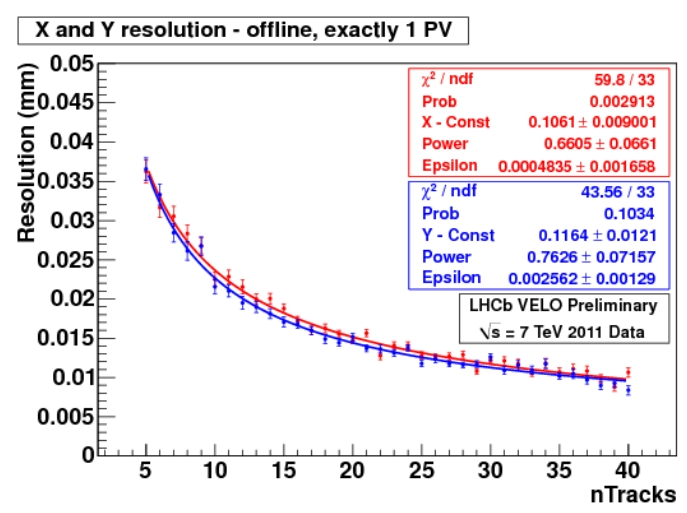
\includegraphics[width=0.49\textwidth]{PVresolution.jpg}}
    \subfigure{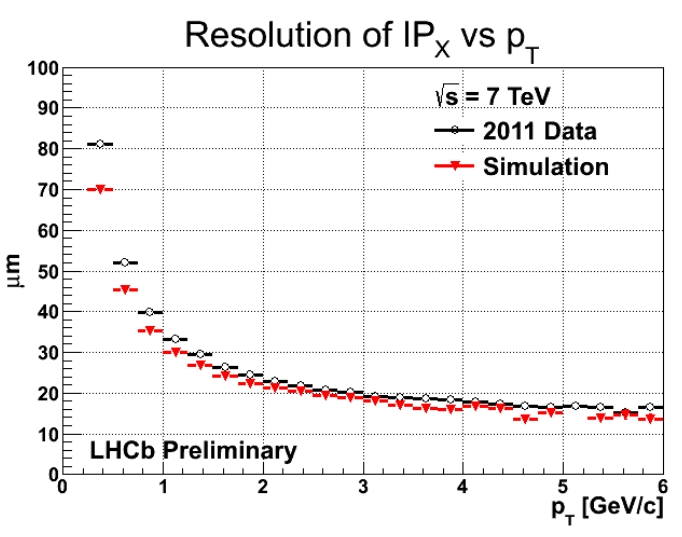
\includegraphics[width=0.49\textwidth]{IPresolution.jpg}}
  \vspace*{-1.0cm}
  \end{center}
  \caption{\textit{Summary of the performance of \lhcb tracking system obtained from 2011 data and Monte Carlo. The primary vertex resolution for the $x$ and $y$ coordinates as a function of the number of tracks (left) and the of the $x$ coordinate of the impact parameter as a function of the transverse momentum $p_T$.}\cite{veloperf}}
  \label{fig:resolution}
\end{figure}
\newpage
%
%
%
\vspace{0.5cm}
\section{The trigger system}
The \lhc collides bunches at a rate of $40 \mhz$. Due to the \lhcb's luminosity levelling the visible\footnote{To be visible, events must have at least two charged particles producing enough hits in the tracking system to be reconstructed.} rate of interaction is $10\mhz$ which has to be reduced to about $4\khz$ to be permanently stored for offline analysis. At \lhcb this is realized by a two-stage trigger system \cite{trigger} \cite{trigger2}: the Level-0 (\lone), a purely hardware based trigger, followed by the High Level Trigger (\hlt) which is executed on a processor farm. A schematic presentation of the trigger system can be seen in in Figure \ref{fig:trigger}.
\begin{figure}[ht]
\vspace*{-0.3cm}
  \begin{center}
    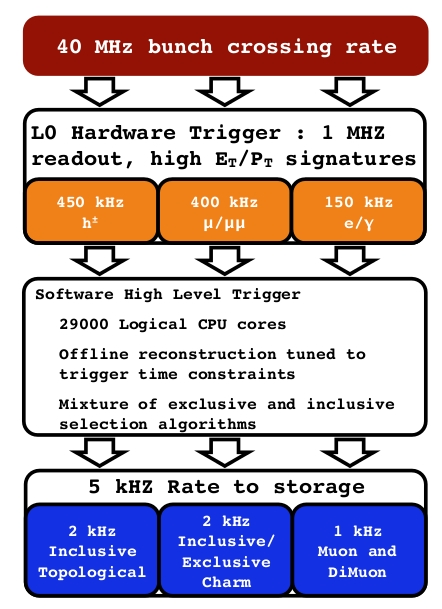
\includegraphics[width=0.43\textwidth]{trigger.jpg}
  \vspace*{-0.5cm}
  \end{center}
  \caption{\textit{A schematic representation of the \lhcb trigger system. The first state is the hardware based Level-0 trigger. Afterwards the High Level Triggers are executed on a processor farm. Each subtrigger uses several trigger lines for dynamic and specific triggering.}}
  \label{fig:trigger}
\end{figure}


\subsection{The Level-0 trigger}
\label{sec:l0}
The \lhcb Level-0 (\lone) trigger is made from custom electronics and reduces the rate from $10\mhz$ to $1\mhz$.\\
To identify events from \B hadrons the \lone trigger makes use of the fact that the large mass of \B hadrons provides a significant amount of transverse kinetic energy to the decay particles. Therefore it selects events with a high amount of transverse energy deposited in the calorimeter or the muon system. Additionally, the \lone accesses information from the \velo pileup and the \spd to reject events with too many tracks. There are different \lone trigger lines for different particles. The two lines important for the analysis are the \lone Electron and the \lone Hadron which will be presented in the following.\\
% Within the bandwidth allocated to the electron trigger (cf. section 7.1.2) the electron Level 0 trigger is required to reject 99\% of the inelastic pp interactions while providing an enrichment factor of at least 15 in b events. This is accomplished through the selection of electrons of large transverse energy ET.  and the \lone TIS (Trigger Independent of Signal)
\newpage
\textbf{The \lone Electron} trigger line is fired by one electromagnetic cluster ($2\times 2$ \ecal cells) with a transverse energy $E_T$ above a threshold value. The electromagnetic cluster must have at least one corresponding hit in the \spd to identify a charged particle opposed to a photon. The threshold value for the transverse energy of the electromagnetic cluster has changed several times over the years 2011 and 2012. This will be evaluated further in Chapter \ref{Chapter4} in Section \ref{sec:triggercat}.\\
\textbf{The \lone Hadron} trigger line is activated by one cluster in the \hcal. The threshold transverse energy $E_T$ for the \lone Hadron is the sum of the transverse energy in the \hcal with the transverse energy the corresponding \ecal cells.
\\
\subsection{The High Level Trigger}
\label{sec:hlt}
All events that pass the \lone trigger will be passed on to the High Level Trigger (\hlt). The \hlt is divided into two levels (\hltone and \hlttwo) which are both implemented as a set of \cpp algorithms run on a CPU farm.\\
\\
Additionally to the information available to the \lone, the \hltone has access to information from the \velo and the tracking system. It reconstructs particles in the \velo and determines the position of the primary vertices in each event. The \hltone then makes a decision based upon impact parameter, momentum, transverse momentum and/or track quality of one track in the event.\\
For each \lone line several \hltone lines are executed. The \hltone reduces the rate to approximately $40 \khz$.\\
\\
All events that pass the \hltone go through to the \hlttwo that performs an event reconstruction similar to the offline analysis. Starting by reconstructing all tracks in the event using the \velo tracks as seed, the \hlttwo reconstructs intermediate particles and resonances and identifies displaced vertices. Afterwards, depending on the \hlttwo line, different sets of selections are applied which are dominantly designed to identify decays of \B and \D hadrons. The \hlttwo finally reduces the rate to about $4\khz$ which is stored for the offline analysis.\\
\\
One \hltone line and several \hlttwo lines will be used in the analysis of the\\ \BdKstee decay. The \hltone line that is used, is the  \textit{Hlt1TrackAllL0Decision} line. This line selects events with at least one track with a high transverse momentum $p_T$ and a great impact parameter (IP) with respect to the primary vertex, since this track is likely to come from a decaying \B hadron.\\
The \hlttwo lines that are used are the \textit{\hlttwo topological lines} \cite{hlt2topo}. These have been designed to trigger inclusive $n$-body ($n = 2,3,4$) \B decays. The \hlttwo lines implement a $Boosted Decision Tree$ to determine if $n$ tracks show the topology of a \B decay. Missed tracks are compensated for by tacking into account the difference between the total momentum of the $n$ tracks and the momentum of the hypothetical \B hadron.\\
\newpage

\section{The \lhcb stripping}
In order to reduce computing time, all events are preselected by a certain \textit{stripping line}. A stripping line consists of a loose selection aiming at rejecting as much background as possible while keeping as much signal as possible. Each decay studied at \lhcb has its own stripping line. All stripping lines are run on the entire dataset regardless of the trigger decision. The stripping is executed by the physics analysis software \davinci (see Section \ref{sec:software}).\\
During the stripping procedure every event is scanned for tracks that can be combined (see Chapter \ref{chapter3}) to make the signal decay. Events with signal candidates are stored for later use.\\

\section{The \lhcb software}
\label{sec:software}
The data processing at \lhcb goes through a series of steps which are executed by different software frameworks. To ensure consistency between these frameworks and the way that data and Monte Carlo are treated, all \lhcb core software is embedded in the \gaudi framework \cite{gaudi}.\\
There are four main applications, each responsible for a different stage of event processing:
\\
\begin{itemize}
\item \textbf{\gauss}is used for the generation of Monte Carlo. Therein, proton-proton collisions are simulated with \pythia \cite{pythia}, the decay of \B hadrons is made with \evtgen \cite{evtgen} and the detector simulation is implemented in \geant \cite{geant}.\\
\item \textbf{\boole}takes the output from \gauss and simulates the digitization of data to give it the same format as the \lhcb data obtained by the electronics and data acquisition systems.\\
\item \textbf{\brunel}performs subdetector and global reconstruction using pattern recognition for both Monte Carlo and real data.\\
\item \textbf{\davinci}executes the last step, namely the reconstruction of the final signal events and running the stripping \cite{davinci}(more details in Chapter \ref{chapter3}).
\end{itemize}

%\textbf{The \lone TIS trigger line}
%All decays that were not triggered by one of their own tracks but later on selected by the Stripping (see Section \ref{sec:stripping}) are called TIS events because the events was triggered independently from the signal by another track in the events, coming from the other \B hadron for example. The \lone TIS decays are most free from any trigger systematics and the trigger efficiency is independent of the decay which is absolutely not the case for the other trigger lines.\\
%\chapter{Study of the reconstruction of the \BdKstee invariant mass}
\chaptermark{Chapter4}
\label{chapter3}
%\addcontentsline{toc}{chapter}{Study of the reconstruction of the \BdKstee invariant mass}
The event reconstruction is a crucial part of the analysis of any decay. At \lhcb, the offline event reconstruction is made in two steps. The first step is executed by the software \brunel that performs subdetector and global reconstruction using pattern recognition for both Monte Carlo and real data. \brunel takes the detector information and reconstructs \textit{tracks} from the hits. The information for each \textit{track} is then stored for further analysis.\\
The second step, the one accessible and adjustable by every user, is executed by the \davinci physics and analysis framework. At the beginning of every event reconstruction \davinci builds lists of \textit{particles}. For each particle-type, such as electron or kaon, there are several lists ranging from very loose to very tight requirements on the \textit{tracks}. For each list, \davinci selects all the \textit{tracks} provided by \brunel that fulfil the list conditions and fully reconstructs them as \textit{particles}, quantities of physics with a four-momentum. In the course of this reconstruction the mass of the \textit{particle} is fixed to the particle-type's mass defined by the list.
%These \textit{particles} are made from the \textit{track} information provided by \brunel and are quantities of physics with a four-momentum. In the course of computing the \textit{particles} properties their masses are fixed to the value corresponding to the condition of the list, e.g. all particles in the list \textsc{SdtAllLooseKaons} have a mass of $493 \mevcc$.\\
From the lists of \textit{particles} \davinci reconstructs intermediate particles (e.g. \Kstarz from \Kp and \pim) and finally the entire \BdKstee decay. \davinci allows the user to choose the \textit{particle} lists and the algorithms that compute their properties, additionally to the way the \textit{particles} are being combined.\\ % einfuegen von bezug auf arbeit
\\
The greatest difficulty in reconstructing the \BdKstee decays is the measurement of the electron\footnote{Throughout this chapter electron stands for electrons and positrons if not mentioned otherwise.} energy. This difficulty arises from bremsstrahlung radiation and propagates to a vast degradation of the \Bd mass resolution. The effects occurring due to bremsstrahlung of the electrons and the means of limiting the loss in precision -- namely different event reconstruction tools implemented in the \davinci framework -- are presented in the following Section. \\
In Section \ref{sec:DiElectronMaker} the focus is put on the reconstruction on the invariant mass of the electron pair $M_{inv}(\epem)$.\\
\newpage
\section{Bremsstrahlung radiation}
\label{sec:bremsstrahlung}
When traversing the material of the detector charged particles undergo a probability of emitting bremsstrahlung. The cross-section for bremsstrahlung emission $\sigma_{bs}$ is anti-proportional to the square of the charged particle's mass $m$ \cite{WRLeo}.
\begin{equation}
 d\sigma_{bs} \propto \frac{e^2}{(mc^2)^2}
\end{equation}
Since the amount of material is low in \lhcb the probability of emitting bremsstrahlung photons is negligible for heavier particles, but very light particles such as electrons and positrons can lose a significant amount of energy through bremsstrahlung radiation. The amount of energy emitted through bremsstrahlung for muons $E_{bs}^{\mmu}$ for instance, is suppressed by a factor $40\ 000$ with respect to that of electrons $E_{bs}^{\electron}$.
\begin{equation}
\frac{E_{bs}^{\electron}}{E_{bs}^{\mmu}} = \frac{m_{\electron}^2}{m_{\mmu}^2} = 2.3 \cdot 10^{-5} 
\label{eq:evsmu}
\end{equation}
%At energies below a few \gev only electrons emit a significant amount of bremsstrahlung radiation in the \lhcb detector.\\
The radiated energy spectrum for the electrons from \BdKstee before the \lhcb magnet is shown in Figure \ref{fig:totalEnergyLossBrems}. The distribution was obtained by performing a Fast-Sim \cite{ananote} on Monte Carlo at simulation level under the assumption of complete screening \cite{pdg}.
\begin{figure}[ht]
  \begin{center}
    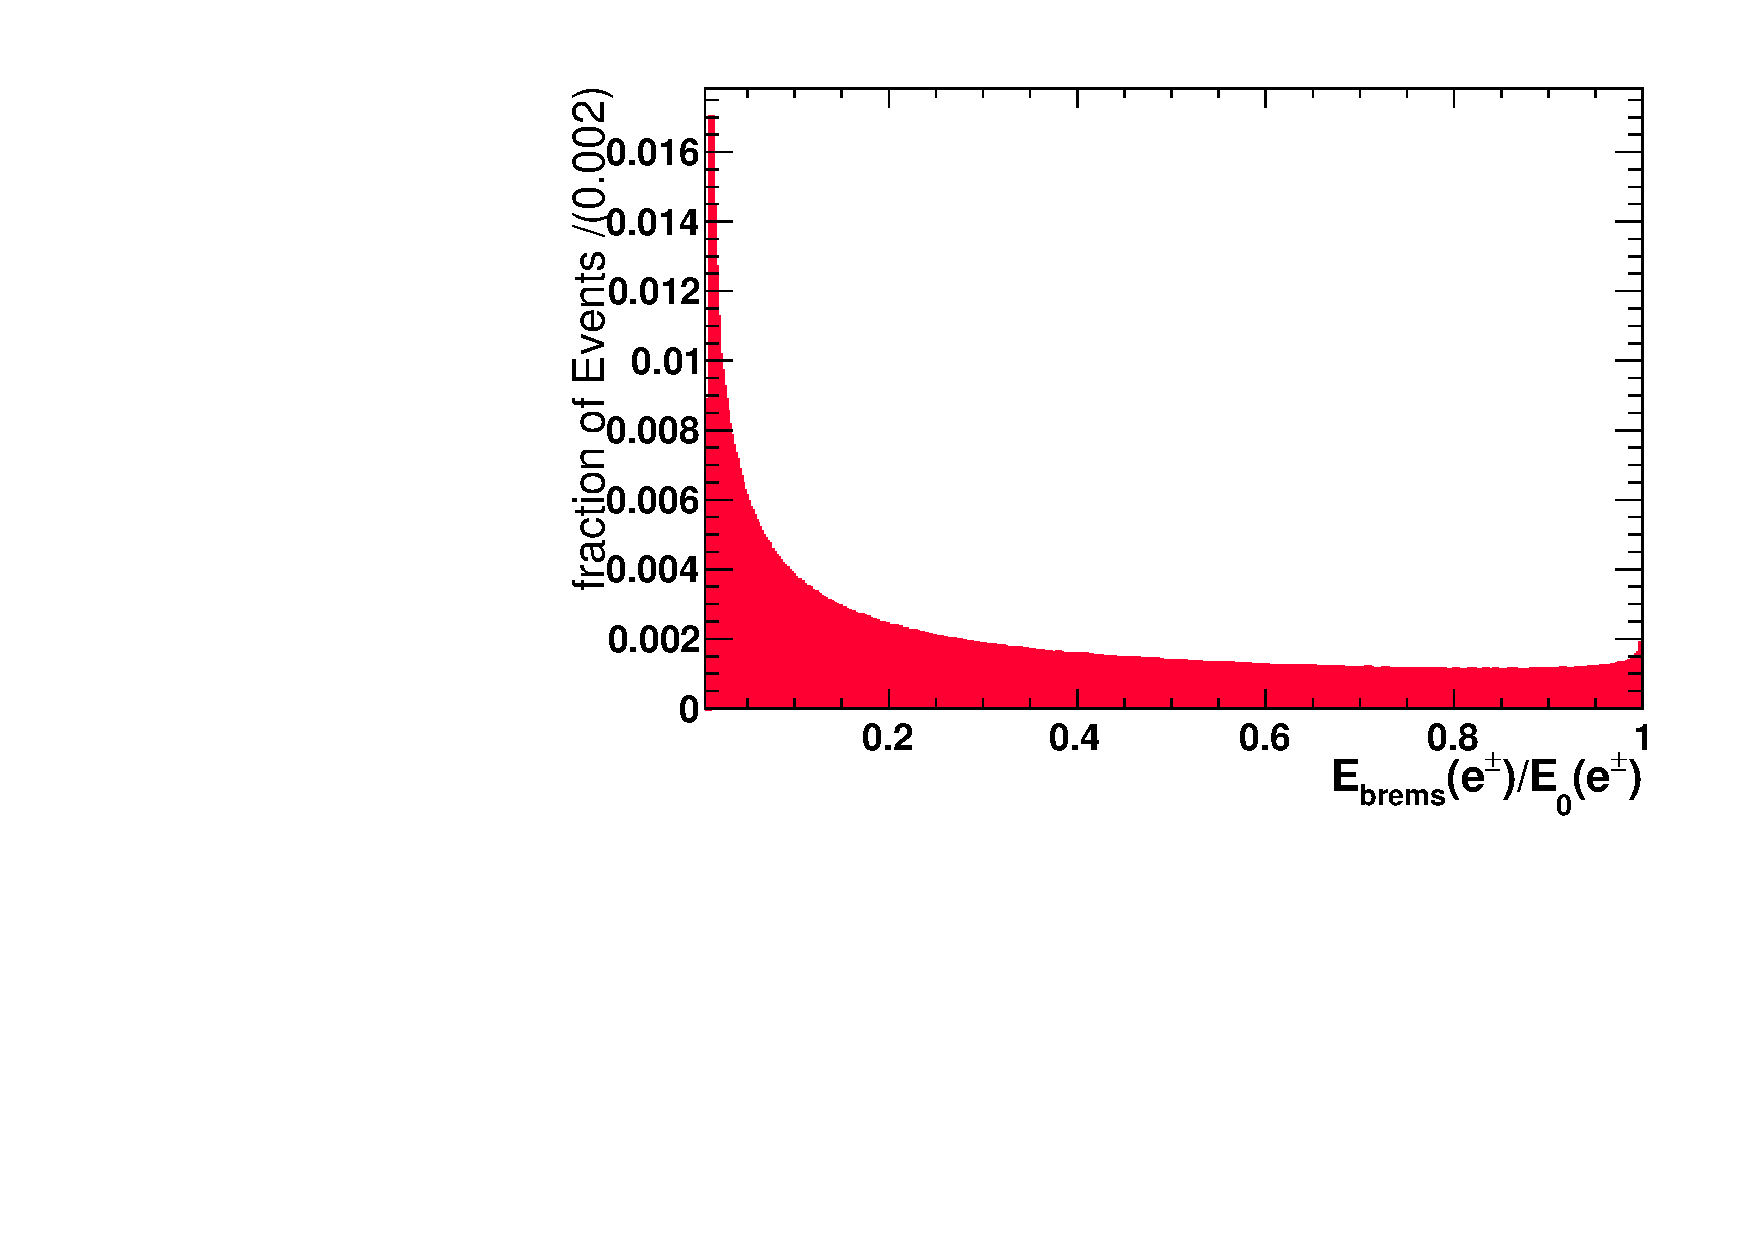
\includegraphics[width = 0.55\textwidth]{EnergyLossBrems.pdf}
    \end{center}
    	\vspace*{-0.8cm}
  \caption{\textit{Percentage of energy loss of electrons/positrons traversing the \lhcb detector before the magnet. $E_{brems}(\epm)$ denotes the energy radiated by the electron/ positron while $E_0(\epm)$ stands for the initial electron/positron energy. Distribution obtained by performing a Fast-Sim on Monte Carlo Data at simulation level under the assumption of complete screening.}}
  \label{fig:totalEnergyLossBrems}
\end{figure}

The bremsstrahlung radiation process is of statistical nature. Figure \ref{fig:totalEnergyLossBrems} shows the amount of radiated energy. It is therefore crucial to identify photons in the detector that have been emitted by electrons through bremsstrahlung radiation and add their four-momentum to the four-momentum of the electron track. The \Bd mass distribution without any kind of bremsstrahlung reconstruction can be seen in Figure \ref{fig:noBremReco}.
\newpage
\begin{figure}[ht]
  	\centering
    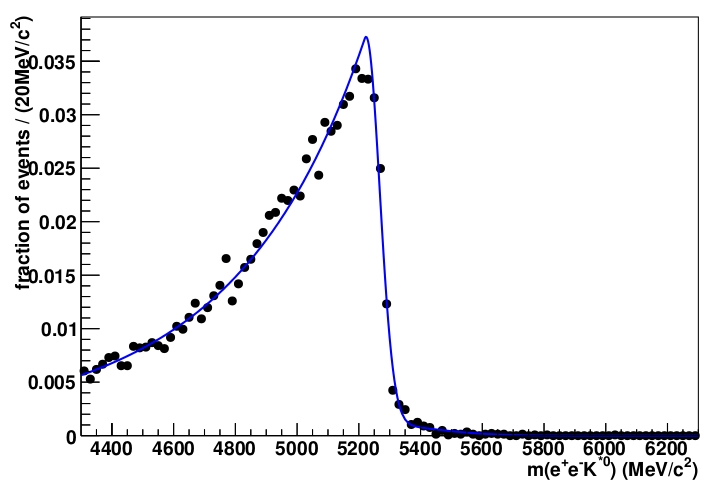
\includegraphics[width = 0.55 \textwidth]{oldBrem_noBremReco.jpg}
  \caption{\textit{The \Bd mass distribution of \BdKstee \lhcb Monte Carlo without any reconstruction of bremsstrahlungs photons.}}
  \label{fig:noBremReco}
\end{figure}

\subsection{Bremsstrahlung recovery}
\label{sec:bremsstrahlungrecovery}
If the emission of the bremsstrahlung happens before the magnet, the electron will be deflected from its initial trajectory by the magnetic field while the bremsstrahlung photon's momentum will not change, as shown in Figure \ref{fig:bremsstrahlung}. Thus, the electron and its photon will deposit their energies in different positions in the \ecal. To allow nonetheless for an assignment of the bremsstrahlung photon with its electron \textit{bremsstrahlung recovery algorithms} have been developed. These algorithms search for bremsstrahlung photon candidates in the \ecal and try to match them to the corresponding electron track.Two different bremsstrahlung recovery algorithms implemented in the \lhcb physics analysis framework will be presented in Sections \ref{sub:oldBrem} and \ref{sub:newBrem}.
\begin{figure}[ht]
\vspace*{-0.4cm}
  \begin{center}
    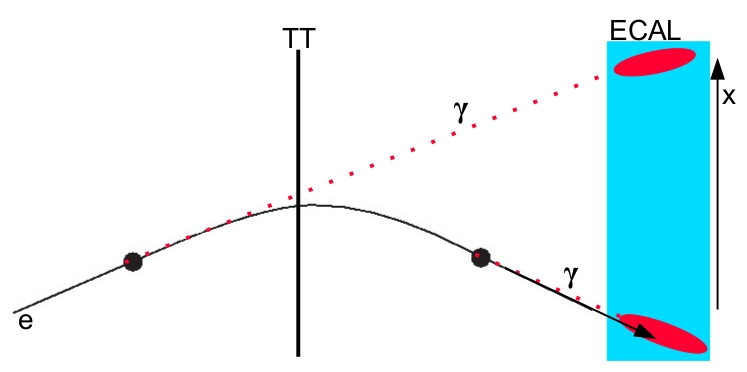
\includegraphics[width=0.6\textwidth]{BremReco.jpg}
  \end{center}
  \vspace*{-0.5cm}
  \caption{\textit{Schematic illustration of bremsstrahlung emission of electrons in the \lhcb detector.}}
  \label{fig:bremsstrahlung}
\end{figure}
If the emission of the bremsstrahlung happens after the magnet, the electron and its photon will deposit their energies in the same \ecal cells. Thus the photon energy is automatically added to the energy of its electron. \\


\subsubsection{Bremsstrahlung recovery algorithm in \davinci v29 }
\label{sub:oldBrem}
The first bremsstrahlung recovery tool was the standard algorithm implemented in all version of \davinci up to v29. An illustration of its methodology is shown in Figure \ref{fig:oldBremAdd}.
\begin{figure}[ht]
\vspace*{-0.5cm}
  \begin{center}
  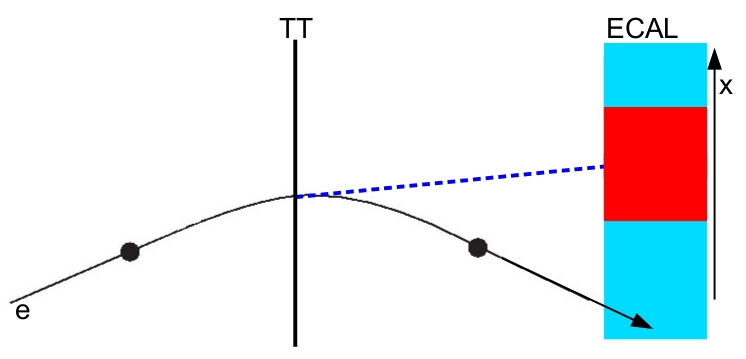
\includegraphics[width=0.6\textwidth]{oldBremAdder.jpg}
  \end{center}
  \vspace*{-0.5cm}
  \caption{\textit{Schematic illustration of the bremsstrahlung recovery algorithm \davinci v29. Black line: curve of the electron track. Dark blue dotted line: linear extrapolation of the electron track from its very first state to the \ecal. Clear blue dotted line: linear extrapolation of the electron track from its last state before the magnet to the \ecal. Red area in the \ecal: area from where photon candidates will be matched to the electron track.}}
  \label{fig:oldBremAdd}
\end{figure}
The algorithm starts with a \textit{particle} list of electrons and searches for reconstructed photon candidates coming from the electron tracks.
To predict the position of bremsstrahlung photon candidates in the \ecal, the algorithm linearly extrapolates the electron track from the \ttracker (last state before the magnet) to the \ecal. All neutral clusters in the \ecal whose barycentric positions match the position of the extrapolated electron track with a $\chi^2 < 300$ are accepted as bremsstrahlung photons. Their four-momentum is added to the four-momentum of the electron. Furthermore there is no limit of bremsstrahlung photon candidates that can be added to one electron.\\


\subsubsection{Bremsstrahlung recovery algorithm in \davinci v30}
\label{sub:newBrem}
The second bremsstrahlung recovery tool is implemented in \davinci v30. Its methodology is illustrated in Figure \ref{fig:newBremAdd}.
\begin{figure}[ht]
  \begin{center}
  \label{fig:newBremAdder}
  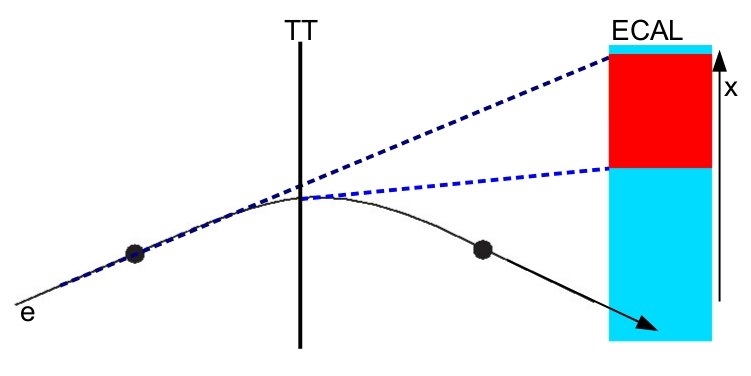
\includegraphics[width=0.6\textwidth]{newBremAdder.jpg}
  \end{center}
  \vspace{-0.8cm}
  \caption{\textit{Schematic illustration of the bremsstrahlung recovery algorithm \davinci v30. Black line: curve of the electron track. Dark blue dotted line: linear extrapolation of the electron track from its very first state to the \ecal. Clear blue dotted line: linear extrapolation of the electron track from its last state before the magnet to the \ecal. Red area in the \ecal: area from where photon candidates will be matched to the electron track.}}
  \label{fig:newBremAdd}
\end{figure}
For each \textit{particle} in the electron list two linear extrapolations of the track are computed, namely the extrapolation of the electron track from its very first state in the \velo to the \ecal and from its state in the \ttracker to the \ecal. Photon candidates must satisfy tighter conditions than for the algorithm in \davinci v29 \footnote{Photon candidates for the \davinci v30 bremsstrahlung recovery algorithm must satisfy the conditions of a PhotonID greater than $-0.5$ and a $p_T$ greater than $75 \mevc$.}.
The $x$ position of the photon candidates in the \ecal must lie between the $x$ positions of the two electron track extrapolations within $\pm 2 \sigma_{x}$. The $y$ position of the photon candidate in the \ecal must match the $y$ position of the electron track extrapolations within $\pm 2 \sigma_{y}$. The $\sigma_{x,y}$ denote the square root of the quadratic sum of the photon cluster spread with the error on the electron track extrapolations. \\



\subsection{The mechanism of double counting}
\label{sec:doublecounting}
Both bremsstrahlung recovery algorithms implemented in \davinci have the disadvantage of generating \textit{double counting}. Double counting occurs when one bremsstrahlung photon candidate can be associated to more than one electron track. This happens particularly often for the \BdKstee decay mode where the $e^+e^-$ invariant mass is very low, yielding small angles between the electron and the positron, as is illustrated in Figure \ref{fig:schemdc}. The distribution of double counting events depending on the $M_{inv}(e^+e^-)$ is shown in Figure \ref{fig:Minveedouble counting}. In the case of double counting the bremsstrahlung recovery algorithms add the photon's four momentum to both the electron's and the positron's four momentum. In the case of \BdKstee, these events will show a non-physically high $B^0$ mass and lead to a non-typical symmetric \Bd mass distribution that can be seen in Figure \ref{fig:oldBremAddernodcc}. 
\begin{figure}[ht]
\vspace*{-0.5cm}
  \begin{center}
  \label{fig:newBremAdder}
  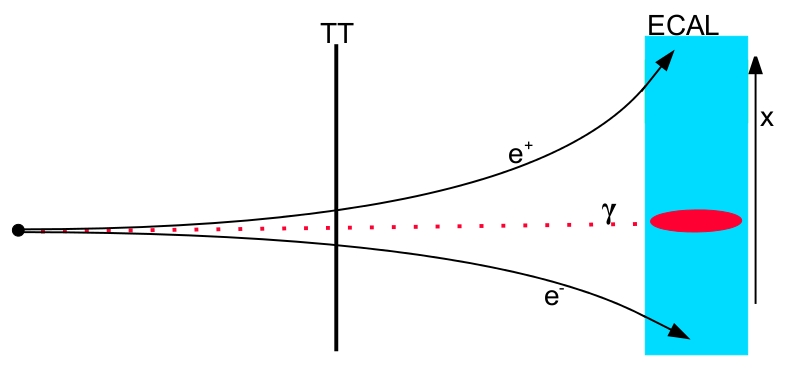
\includegraphics[width=0.6\textwidth]{doublecounting.jpg}
  \end{center}
  \vspace*{-0.5cm}
  \caption{\textit{Schematic illustration of the mechanism of double counting. Due to a very low $e^+e^-$ invariant mass the angle between the electron and the positron is so small that the photon can be associated to both.}}
  \label{fig:schemdc}
  \vspace*{-0.5cm}
\end{figure}

\begin{figure}[ht]
  \begin{center}
  \vspace*{-.6cm}
  \subfigure{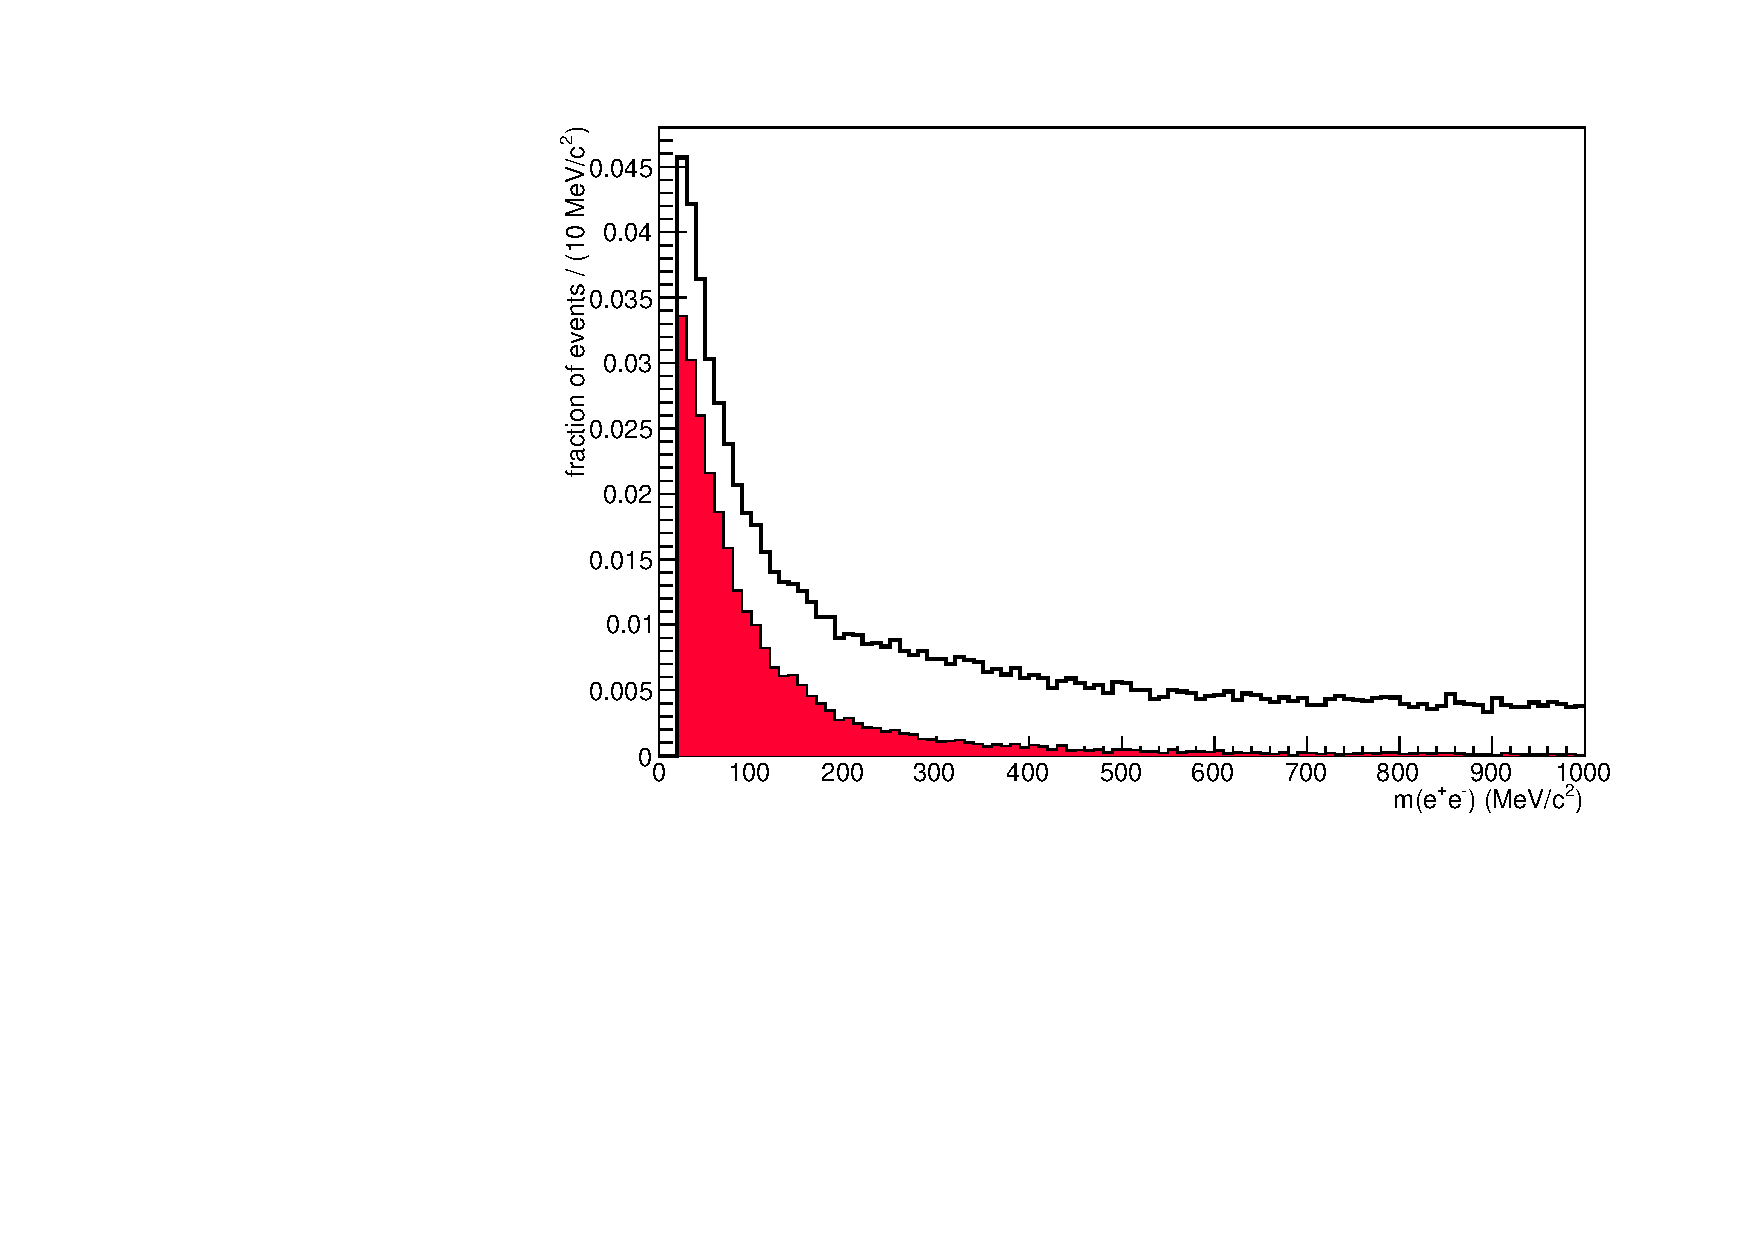
\includegraphics[width=0.48\textwidth]{dccats_Minvee_oldBrem.pdf}}
    \subfigure{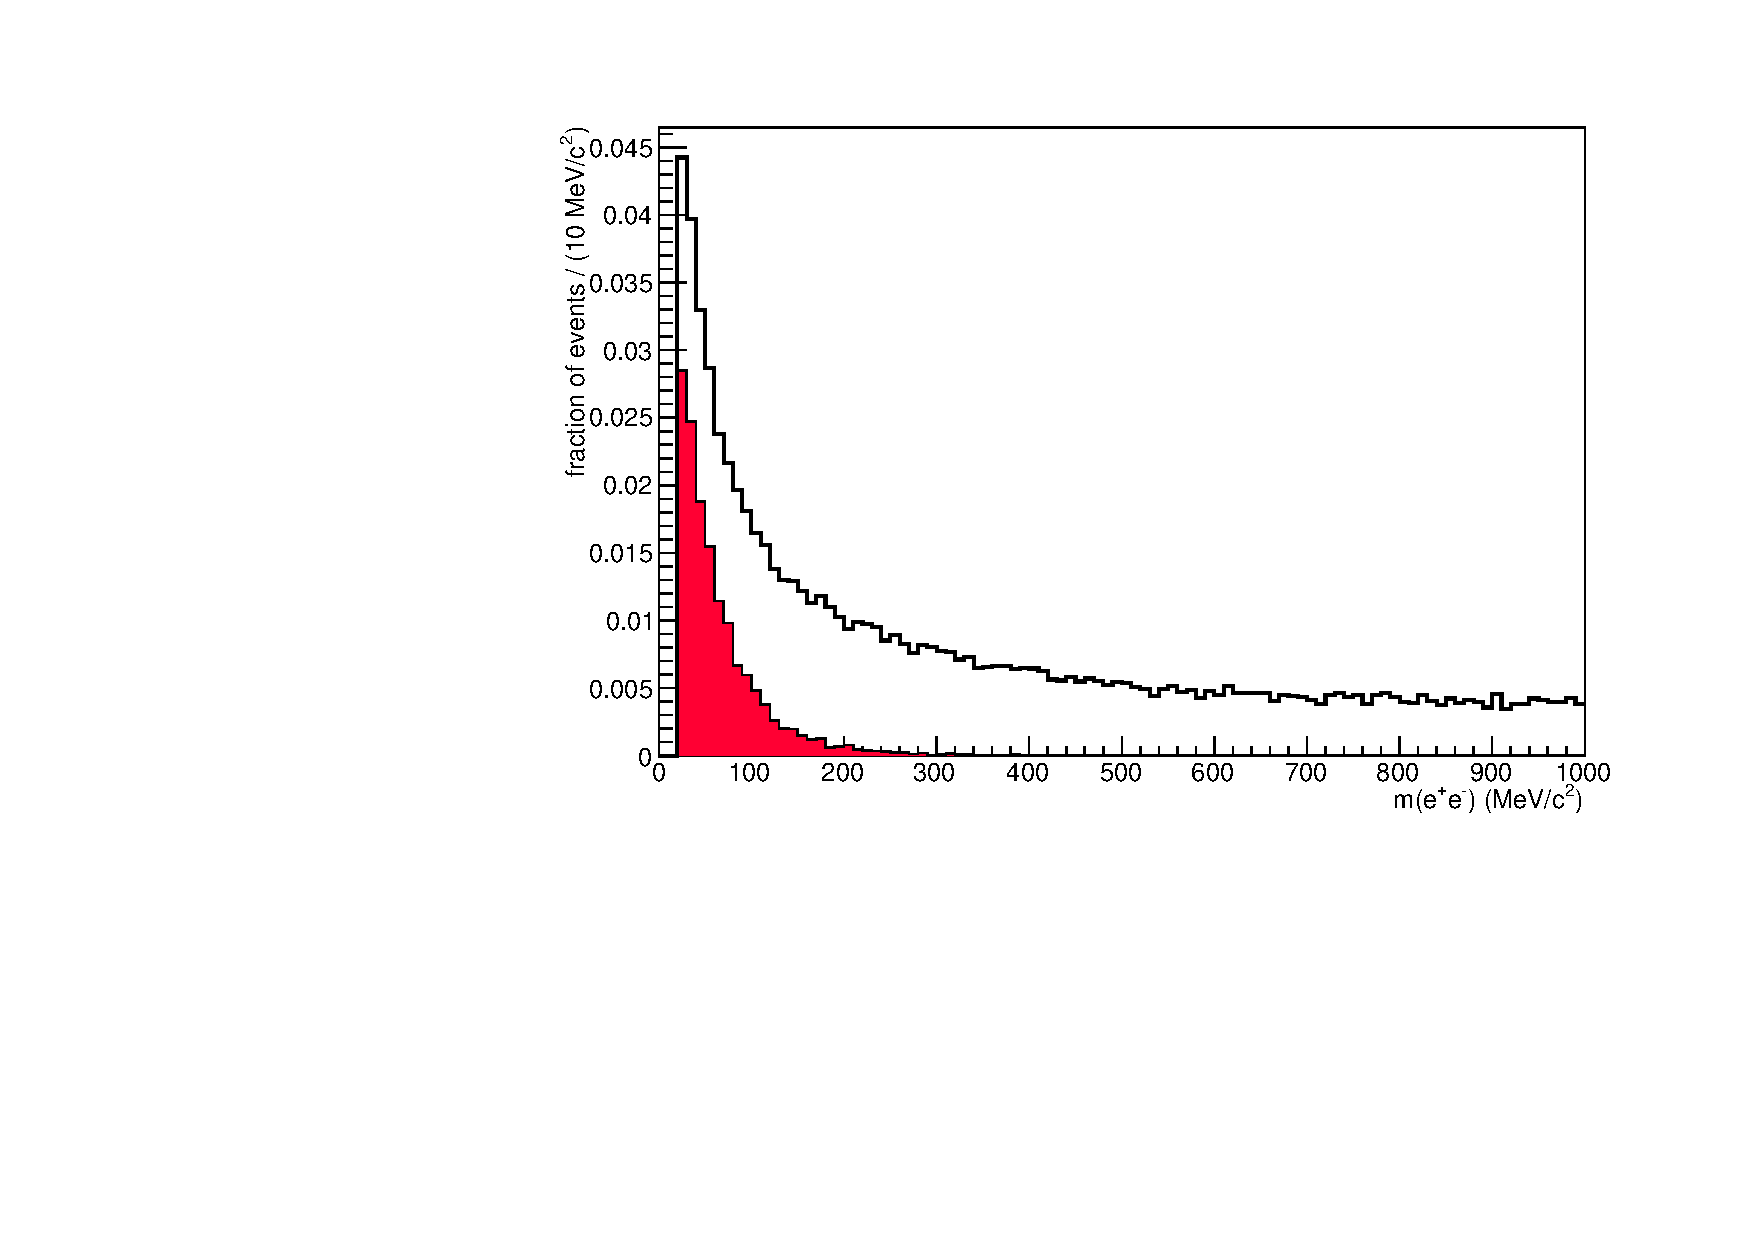
\includegraphics[width=0.48\textwidth]{dccats_Minvee_newBrem.pdf}}
  \vspace*{-1.0cm}
  \end{center}
  \caption{\textit{$M_{inv}(e^+e^-)$ distribution obtained by reconstructing \lhcb Monte Carlo with \davinci v29 (left) and \davinci v30 (right) respectively.. The pink distribution are the events with double counting.}}
  \label{fig:Minveedouble counting}
  \vspace*{-0.5cm}
\end{figure}


\begin{figure}[ht]
\vspace*{-0.5cm}
  \begin{center}
  \subfigure{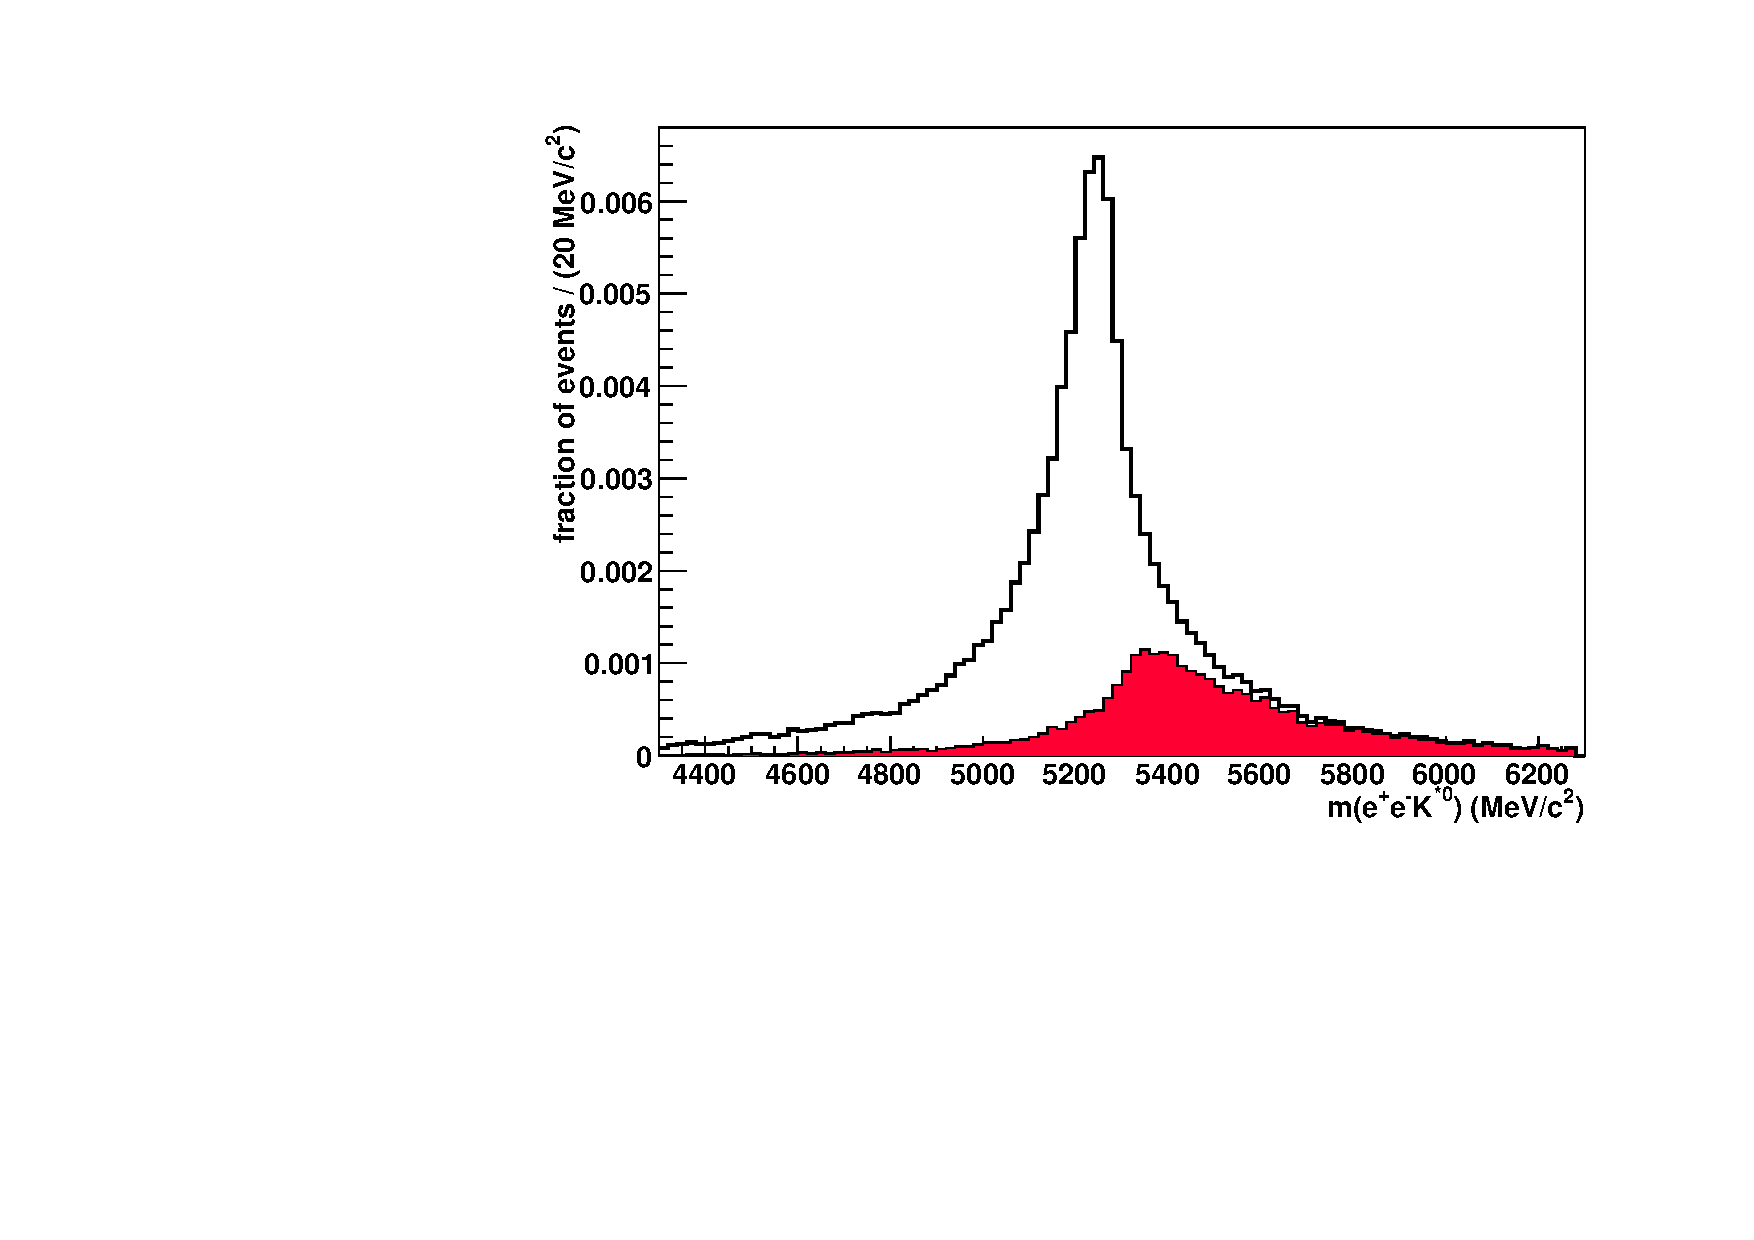
\includegraphics[width=0.49\textwidth]{MC_Bmass_dielectron_TM_nodccorrection_simplehisto.pdf}} 
  \subfigure{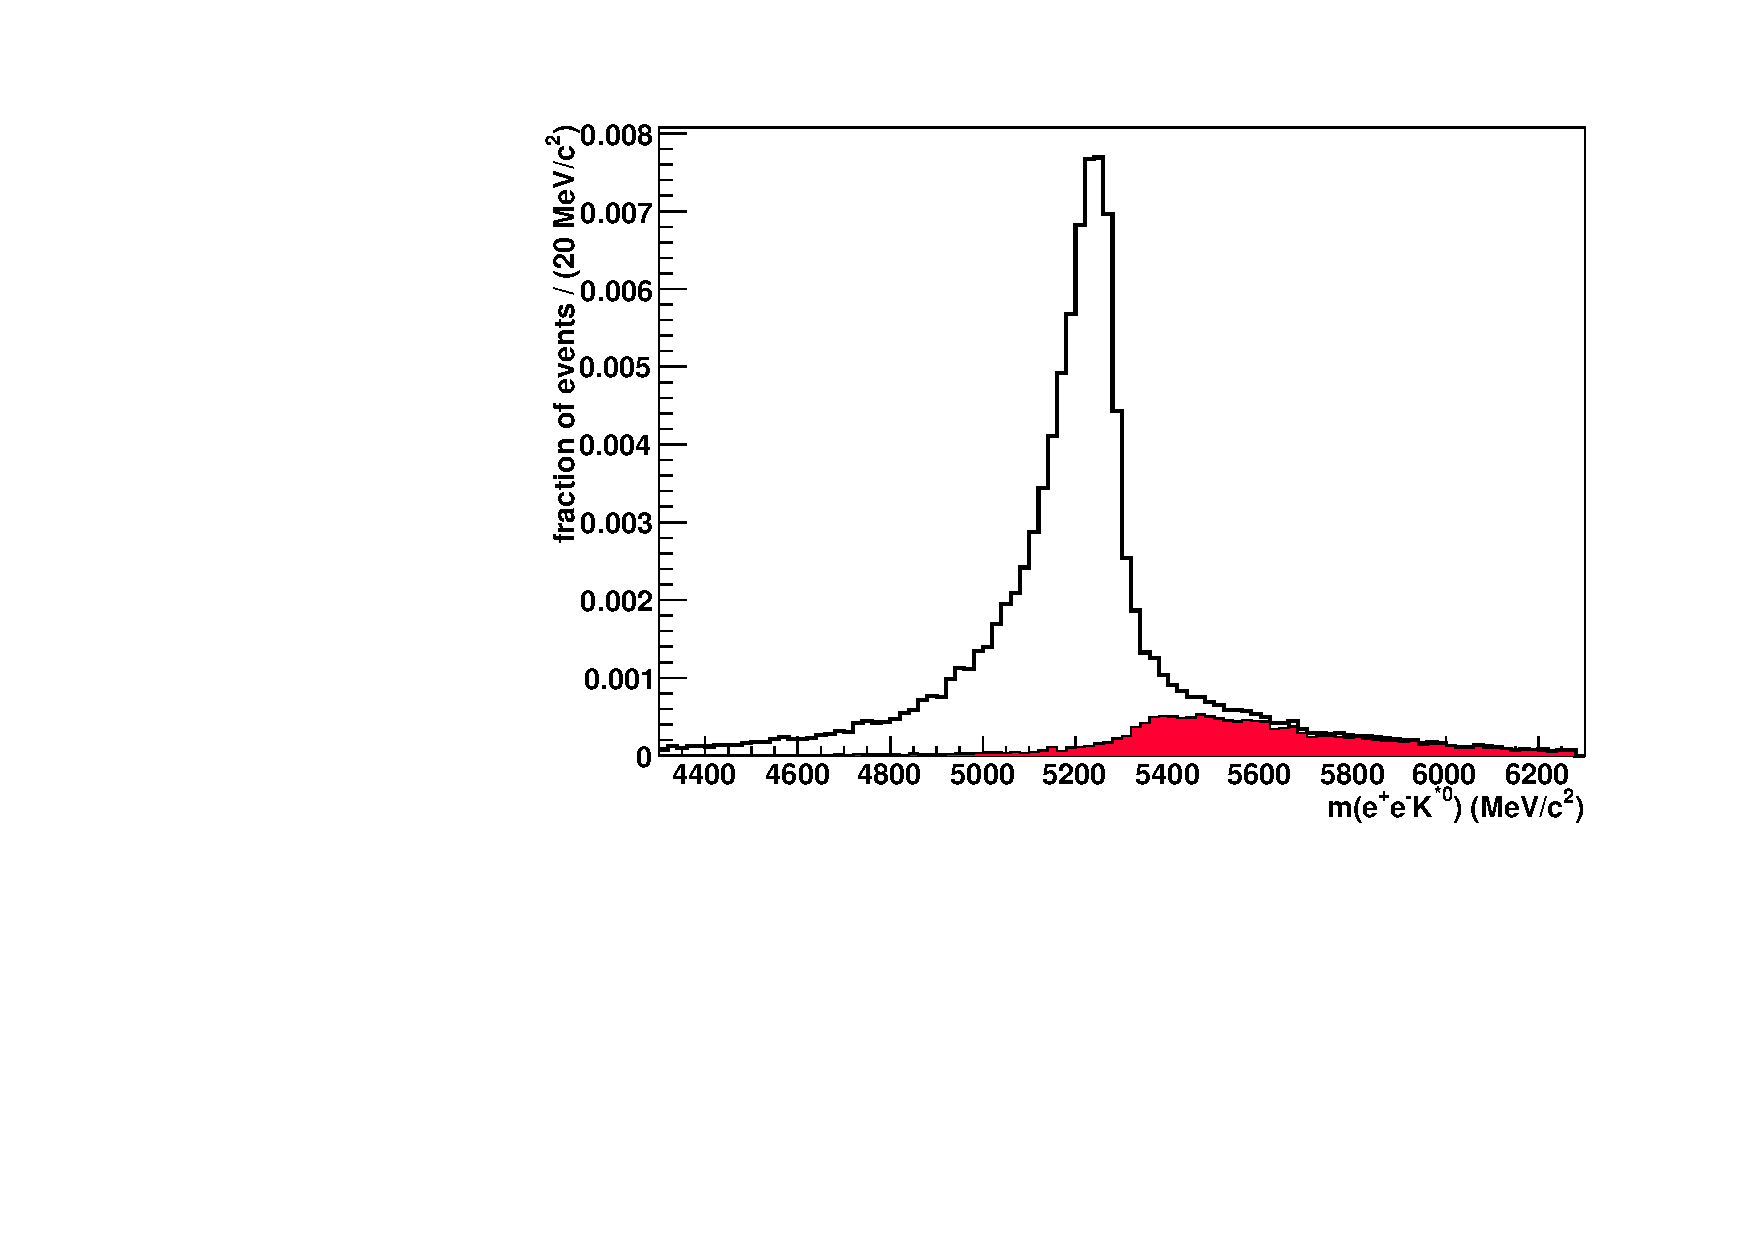
\includegraphics[width=0.49\textwidth]{MC_Bmass_dielectron_TM_nodccorrection_simplehisto_newBrem.pdf}}
  \vspace*{-1.0cm}
  \end{center}
  \caption{\textit{\Bd mass shape. The pink distribution are the events with double counting. The \Bd distribution is obtained by reconstructing \lhcb Monte Carlo with \davinci v29 (left) and \davinci v30 (right) respectively.}}
  \label{fig:oldBremAddernodcc}
\end{figure}
As can be seen from Figures \ref{fig:oldBremAddernodcc} and \ref{fig:Minveedouble counting} the amount of double counting is higher for the \davinci v29 bremsstrahlung recovery. The \lhcb Monte Carlo sample shows that double counting events account for 27 \% of all the signal events in \davinci 29 while it's only about 14\% of the signal events for \davinci v30. \\



\subsubsection{The double counting correction}
\label{sub:doublecountingcorrection}
In the course of the analysis four different methods to encounter the problem of double counting have been developed and tested:
\begin{compactenum}[a)]
\item The energy of the double counted photon candidate is assigned to the lepton with lower energy.
\item The energy of the double counted photon candidate is assigned to the lepton with higher energy.
\item The energy of the double counted photon candidate is assigned to a randomly chosen lepton. 
\item The energy of the double counted photon candidate is equally divided between the two leptons.
\end{compactenum}
After assigning the bremsstrahlung photon's energy, the four-momenta of the leptons is recalculated. From these new lepton four-momenta and the original four-momenta of the Kaon and the Pion the \Bd mass is recalculated.\\
The recalculated \Bd mass distributions for the four different methods applied to the \BdKstee \lhcb Monte Carlo sample made with the \davinci v29 are shown in Figure \ref{fig:double countingcorrection}. \\
While the first three methods yield extremely similar results, the fourth method does not reproduce the \Bd mass shape correctly. For further analysis the third method of encountering double counting is chosen. Assigning of the bremsstrahlung photon's energy to one randomly chosen electron does not undergo the risk of biasing any energy distribution and yields the most accurate \Bd mass reconstruction of the four tested algorithms.\\
\begin{figure}[ht]
\vspace*{-0.4cm}
  \begin{center}
    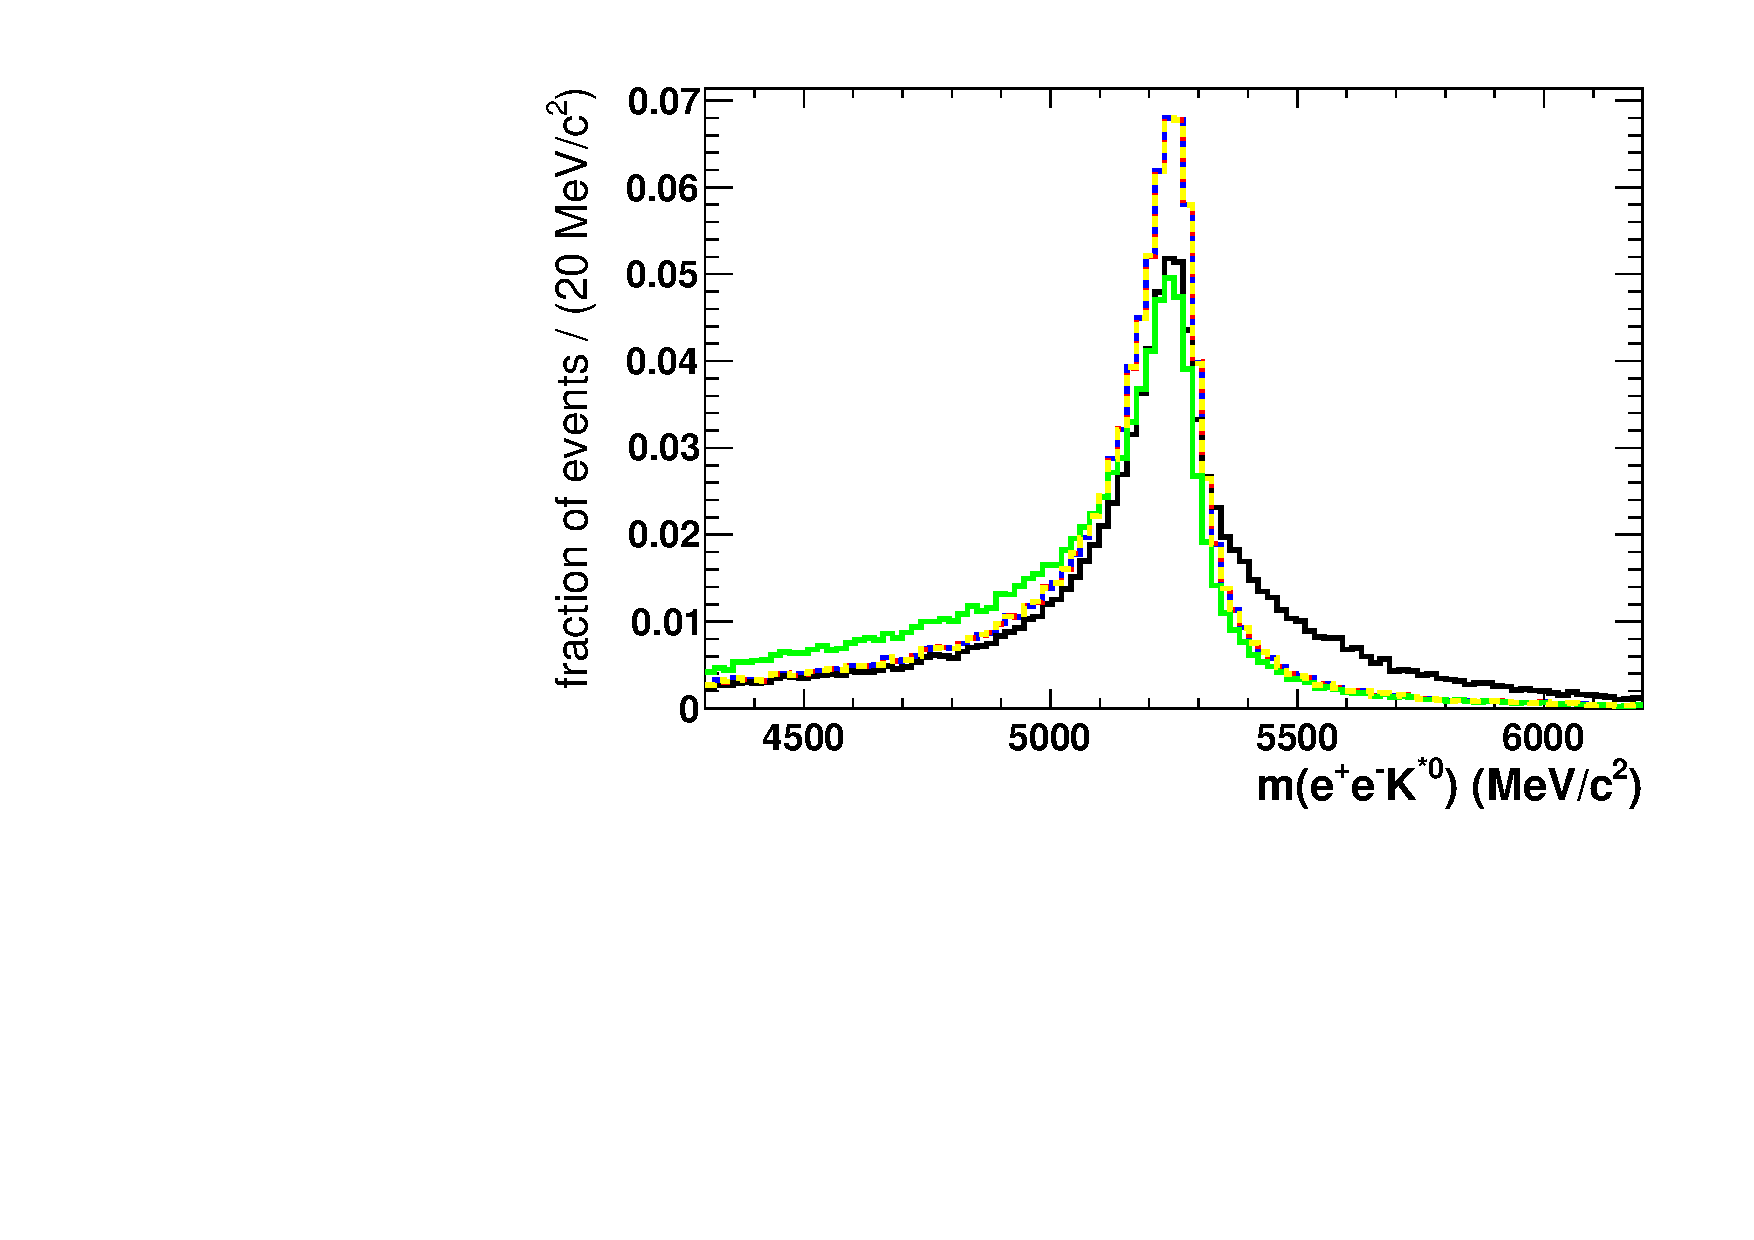
\includegraphics[scale=0.6]{minvB_nodccorrection.pdf}
  \vspace*{-1.0cm}
  \end{center}
  \caption{\textit{\Bd mass shapes for different algorithms of double counting correction. Black: no double counting correction; red: a); yellow: b); blue: c); green: d). }}
  \label{fig:double countingcorrection}
\end{figure}
\\

\subsection{Comparison of bremsstrahlung recovery algorithms}
The two bremsstrahlung recovery tools are applied to the \BdKstee \lhcb Monte Carlo, together with the double counting correction developed in the previous section. Additionally the selection developed for the 2011 dataset \cite{michellesthesis} is applied to the samples to estimate the effects on the final dataset.\\
To quantify the quality of the reconstruction tools a double Crystal-Ball distribution \cite{crystal} (for more details see Section \ref{sec:pdfs}) is fitted to the \Bd mass shape. The two Crystal-Ball distributions share the same $\mu_{\B}$, $\alpha$ and $n$. A weighted width $\sigma^w$ is calculated from the width $\sigma_1$ and $\sigma_2$ from the two Crystal-Ball distributions, where $f$ denotes the relative contribution from the first Crystal-Ball distribution.
\begin{equation}
\sigma^w = f \sigma_1 + (1- f) \sigma_2
\end{equation}

The two resulting distributions can be seen in Figure \ref{fig:comparebrems}. The resulting weighted resolutions are listed in Table \ref{tab:sigmaw}.

\begin{figure}[!h]
\vspace*{-0.cm}
  \begin{center}
  \subfigure{\label{fig:oldBremAdder}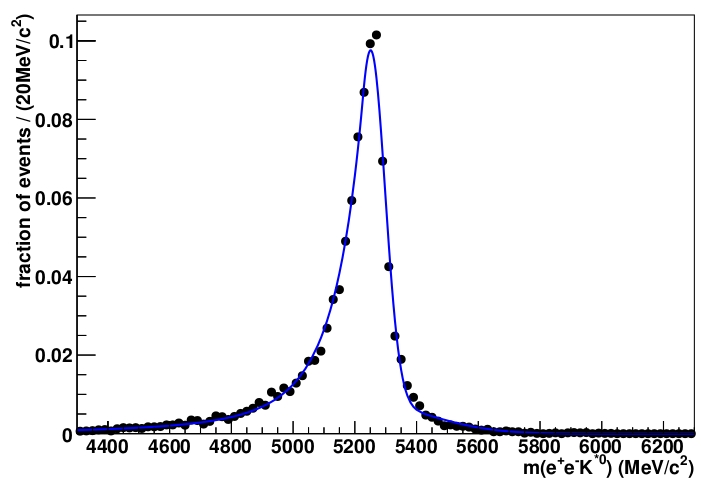
\includegraphics[width=0.49\textwidth]{oldBrem_crystalfit.jpg}}
  \subfigure{\label{fig:newBremAdder}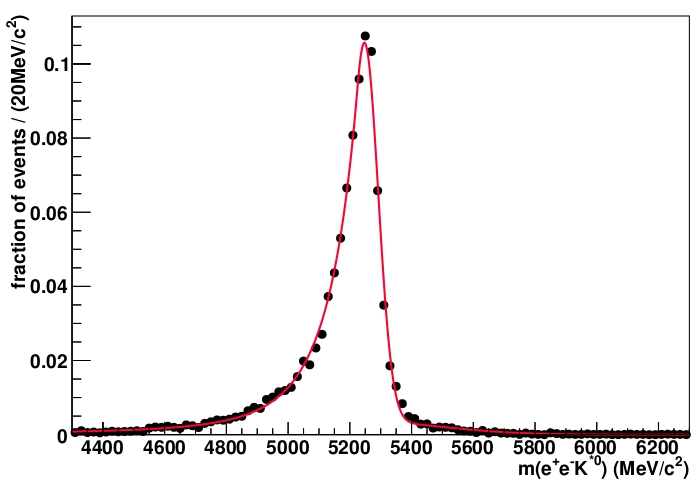
\includegraphics[width=0.48\textwidth]{newBrem_crystalfit.jpg}} 
  \vspace*{-1.0cm}
  \end{center}
  \caption{\textit{\Bd mass distribution obtained from \lhcb Monte Carlo with \davinci v29 (left) and \davinci v30 (right) and the double counting correction.}}
  \label{fig:comparebrems}
\end{figure}

\begin{table}[!h]
\begin{center}
\begin{tabular}{c|c|c|c|c}
& $\sigma_1$ & $\sigma_2$ & $f$ & $\sigma^w$ \\
\hline
\davinci v29 &  47 \mevcc & 199 \mevcc & 0.76 & 83 \mevcc \\
\hline
\davinci v30 & 45 \mevcc & 251 \mevcc & 0.86 & 74 \mevcc \\
\end{tabular}
\end{center}
\vspace*{-0.5cm}
\caption{\textit{Relevant results of the fit of a double Crystal-Ball distribution to the \BdKstee \lhcb Monte Carlo reconstructed with \davinci v29 and \davinci v30 and the double counting correction. $\sigma^w$ denotes the weighted width.}}
\label{tab:sigmaw}
\end{table}
By using the bremsstrahlung reconstruction in \davinci v30, the resolution of the \Bd mass can by increased about $13\ $\%. \\


\subsection{Effect of bremsstrahlung radiation and reconstruction on the \Bd mass shape}
Despite the implementation of the bremsstrahlung recovery tools, bremsstrahlung radiation affects the reconstructed \Bd mass shape. This can be seen in Figure \ref{fig:electronAndMuonBMass} where the reconstructed \Bd from \BdKstee is shown in direct comparison to the distribution of the \Bd mass from \BdKstmumu.\\
One effect is the large tail of the \Bd mass distribution from \BdKstee towards low \Bd masses. This tail originates from events whose bremsstrahlung photons could not be recuperated, resulting in a 
measured electron energy smaller than the initial electron energy $E^{measured}_{\epm} = (1 - E_{bs}) E^0_{\epm}$. \\
The second effect is the downgraded mass resolution which stems from the great uncertainty on the energy measurement of the calorimeter. In \lhcb the energy measurement of charged particle is performed by using combined information from the tracking system and the particle identification system. The tracking system determines the momentum of the charged particle $p_T^{track}$ with a relative accuracy of about $0.5 $\%. The particle identification system determines the identity of the particle which fixes the invariant mass of the particle track to the PDG value $m^{PDG}$. The particle's energy $E$ is then calculated from the combination of the measured momentum and the PDG \cite{pdg} \footnote{Particle Data Group.} mass.
\begin{equation}
E = \sqrt{p^2_{track} + m^2_{PDG}}
\end{equation}
The relative energy resolution is thus also of the order of $0.5 $\%.\\
For neutral particles however, the energy measurement has to be performed by the calorimeter. Since the relative energy resolution of the calorimeter is  
\begin{equation}
\frac{\sigma_E}{E} = \frac{10 \%}{\sqrt{E}} \oplus 1 \%
\end{equation}
the energy resolution of neutral particles is much worse than the energy resolution of charged particles.\\
Electrons, like muons, are charged particles and their tracks' transverse momenta $p_T^{track}(\epm)$ could be determined with an average relative accuracy of $0.5$\%. The energy of the bremsstrahlung photons however, has to be determined by the \ecal. The increase in uncertainty on the electron energy will propagate to the measured \Bd mass. \\
Figure \ref{fig:electronAndMuonBMass} shows the comparison between the \Bd mass shape of the \BdKstee and the \BdKstmumu.
\begin{figure}[ht]
  \begin{center}
  \subfigure{
  	\label{fig:eeKstar}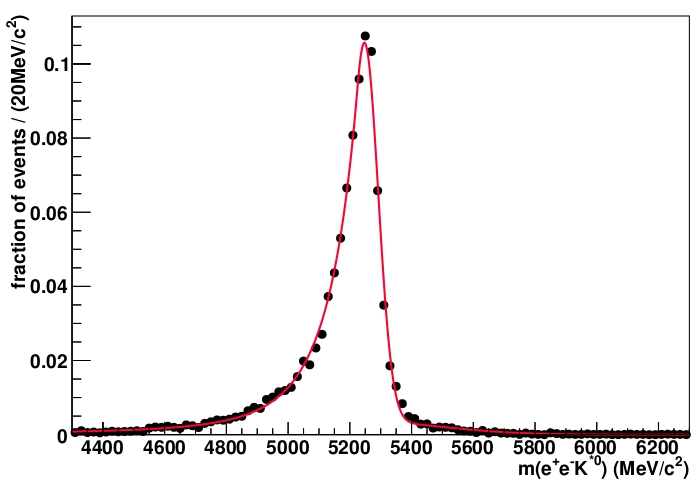
\includegraphics[width=0.49\textwidth]{newBrem_crystalfit.jpg}}
  \subfigure{\label{fig:mumuKstar}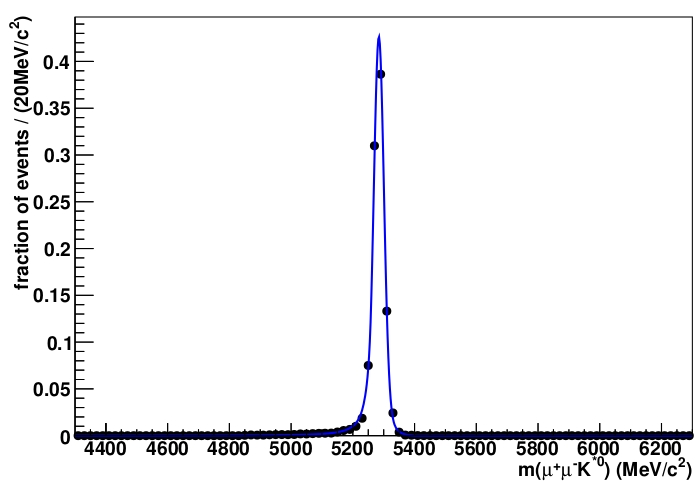
\includegraphics[width=0.49\textwidth]{MC_Bmass_mumuKstar_TM.jpg}} 
  \vspace*{-1.0cm}
  \end{center}
  \caption{\textit{Comparison of the \Bd mass distribution from \BdKstee (left) and \BdKstmumu (right) reconstructed from \lhcb Monte Carlo samples. The distribution from  \BdKstee is much wider and shows a tail at low \Bd masses, while the distribution for \BdKstmumu is just a very narrow peak.}}
  \label{fig:electronAndMuonBMass}
\end{figure}


\section{$M_{inv}(\epem)$ reconstruction}
\label{sec:DiElectronMaker}
The correct reconstruction of the invariant mass of the $e^+ e^-$ pair in the \BdKstee decay is crucial for the measurement of the various amplitudes contributing to the decay since they depend on the $M_{inv}(\epem)$ (see Chapter \ref{chapter1}).\\
In \davinci v31 a new tool designed to make opposite and same sign electron pairs was introduced. This tool -- the so-called \dielectronmaker  \ -- was specially developed to reconstruct low invariant mass $e^+ e^-$ pairs, such as electrons and positrons from converted photon or light resonances.\\
\\
While usually electron pairs are being made by combining two reconstructed electrons, the \dielectronmaker accesses the raw detector information for the electron and the positron candidates directly. Based on the hits associated to the two candidates' tracks the \dielectronmaker creates a \textit{DiElectron object} first and only then computes the properties of the individual electron and positron respectively. The \dielectronmaker chooses tracks with a $p_T$ greater than $100 \mevc$ as electron candidates. It composes the \textit{DiElectron object} from opposite sign electron pair tracks and then applies the bremsstrahlung recovery tool from \davinci v30. In the case of double counting within one \textit{DiElectron object} the four-momentum of the photon candidate is added to one randomly chosen electron, similarly to the double counting correction in Section \ref{sub:doublecountingcorrection}. Then the four-momenta of the \textit{DiElectron object} and the electron and the positron are calculated and a $p_T(e^+ e^-)$ cut greater than $500 \mevc$ is applied.
From this \textit{DiElectron object} the rest of the event reconstruction follows as usual.\\
\\
The \dielectronmaker was created to increase the efficiency of reconstruction for events with low invariant mass $e^+ e^-$ pairs and also yields a more precise reconstruction of the \Bd mass as can be seen on the Monte Carlo sample in Figure \ref{fig:diElectron}. Additionally the selection developed for the 2011 dataset \cite{michellesthesis} is applied to the sample to estimate the effects on the final dataset. The results of the fit of the double Crystal-Ball distribution to the sample are listed in Table \ref{tab:disigmaw}, showing that the use of this new tool decreases the $\sigma^w$ even further than the reconstruction by \davinci v30  yielding a reduction of $27 \ $\% with respect to the reconstruction implemented in \davinci v29.
\begin{figure}[ht]
  \begin{center}
  \subfigure{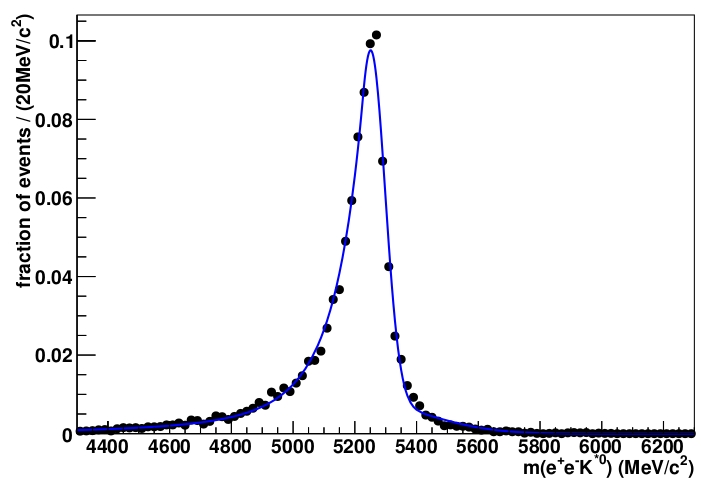
\includegraphics[width=0.49\textwidth]{oldBrem_crystalfit.jpg}}
  \subfigure{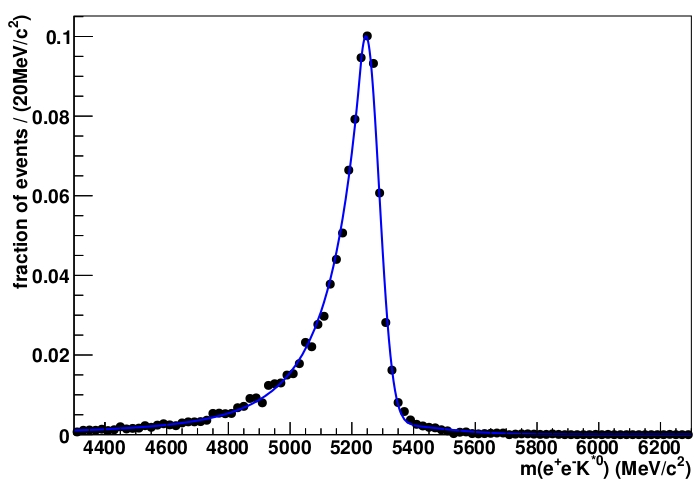
\includegraphics[width=0.49\textwidth]{diElectron_crystalfit.jpg}} 
  \end{center}
  \caption{\textit{\Bd mass distribution obtained from \lhcb Monte Carlo with \davinci v29 and double counting correction (left) and the \dielectronmaker of \davinci v31 (right).}}
  \label{fig:diElectron}
\end{figure}

\begin{table}[hc]
\begin{center}
\begin{tabular}{c|c|c|c|c}
& $\sigma_1$ & $\sigma_2$ & $f$ & $\sigma^w$ \\
\hline
\davinci v29 &  47 \mevcc & 199 \mevcc & 0.76 & 83 \mevcc \\
\hline
\davinci v31 & 54 \mevcc &  306 \mevcc & 0.91 &  77 \mevcc \\
\end{tabular}
\end{center}
\vspace*{-0.5cm}
\caption{\textit{Relevant results of the fit of a double Crystal-Ball distribution to the \BdKstee \lhcb Monte Carlo reconstructed with \davinci v29 and the double counting correction and \davinci v31. $\sigma^w$ denotes the weighted width.}}
\label{tab:disigmaw}
\end{table}

Figure \ref{fig:deltaee} shows the resolution of the dilepton invariant mass obtained from \BdKstee Monte Carlo for a dilepton invariant mass between 20\mevcc and 30\mevcc and 30\mevcc and 50\mevcc respectively. The resolutions are computed for the Monte Carlo sample that was processed with each  \davinci v29 and \davinci v31.\\
The plots show that the histograms from \davinci v31 are better centred and their Root Mean Square (RMS) is reduced by 20\% to 30\%. The first effect originates from the newer Bremsstrahlung recovery algorithm that is implemented in the \dielectronmaker. This recovery algorithm identifies more bremsstrahlung photons than the one in \davinci v29 and adds them to their emitting electron. The use of the \dielectronmaker reduces the RMS of the histograms with respect to those made by \davinci v29 because of the intermediate step of computing the \textit{DiElectron object}.
\begin{figure}[!h]
\vspace*{-0.cm}
  \begin{center}
    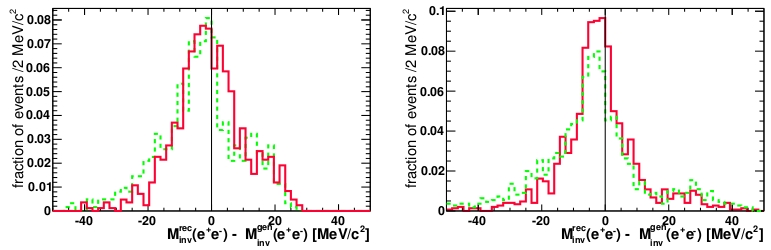
\includegraphics[scale=0.6]{deltaee.jpg}
  \vspace*{-0.5cm}
  \end{center}
  \caption{\textit{Resolution of the dilepton invariant mass obtained from the \BdKstee Monte Carlo. \textbf{Left:} The histograms for the region of 20\mevcc < $M^{gen}_{inv}(\epem)$ < 30\mevcc. \textbf{Right:} The histograms for the region of 30\mevcc < $M^{gen}_{inv}(\epem)$ < 50\mevcc. The green histogram represents the resolution of the sample processed with \davinci v29, the pink histogram represents the resolution of the sample processed with \davinci v31.}}
  \label{fig:deltaee}
\end{figure}
\\
\vspace*{1.cm}
\section{Comparison of reconstruction efficiencies}
To evaluate the performance of $M_{inv}(\epem)$ reconstruction the three reconstruction tools implemented in \davinci v29, \davinci 30 and \davinci v31 are applied to the \BdKstee \lhcb Monte Carlo respectively. After this, the double counting correction algorithm is executed on the first two samples and the selection developed for the 2011 dataset \cite{michellesthesis} \cite{paper} is applied to all three samples to estimate the effects on the final datasets.\\
Figure \ref{fig:eff_diElectron} shows the overall efficiency for reconstruction and selection of the three samples in dependency of the true -- that is generated -- invariant \epem mass $M^{gen}_{inv}(\epem)$. Note that there is a cut on the reconstructed invariant \epem mass $M^{reco}_{inv}(\epem)>30 \mevcc$\footnote{The selection developed for the 2011 dataset \cite{michellesthesis} \cite{paper} includes a tighter cut on the invariant dilepton mass than the selection developed in the course of this master's thesis}.\\
Figure \ref{fig:eff_diElectron} shows that the use of the \dielectronmaker yields the most accurate results and the highest reconstruction efficiency, especially in the region of highest interest between $30 \mevcc$ and $65 \mevcc$. The amount of reconstructed events with a generated invariant mass below $30 \mevcc$ is zero up to almost $15 \mevcc$ and then smoothly increases due to multiple scattering.\\
Above $65 \mevcc$ the efficiencies for all three reconstruction algorithms converge to the same value and remain independent of the generated invariant \epem mass.\newpage
\begin{figure}[!h]
  \begin{center}
    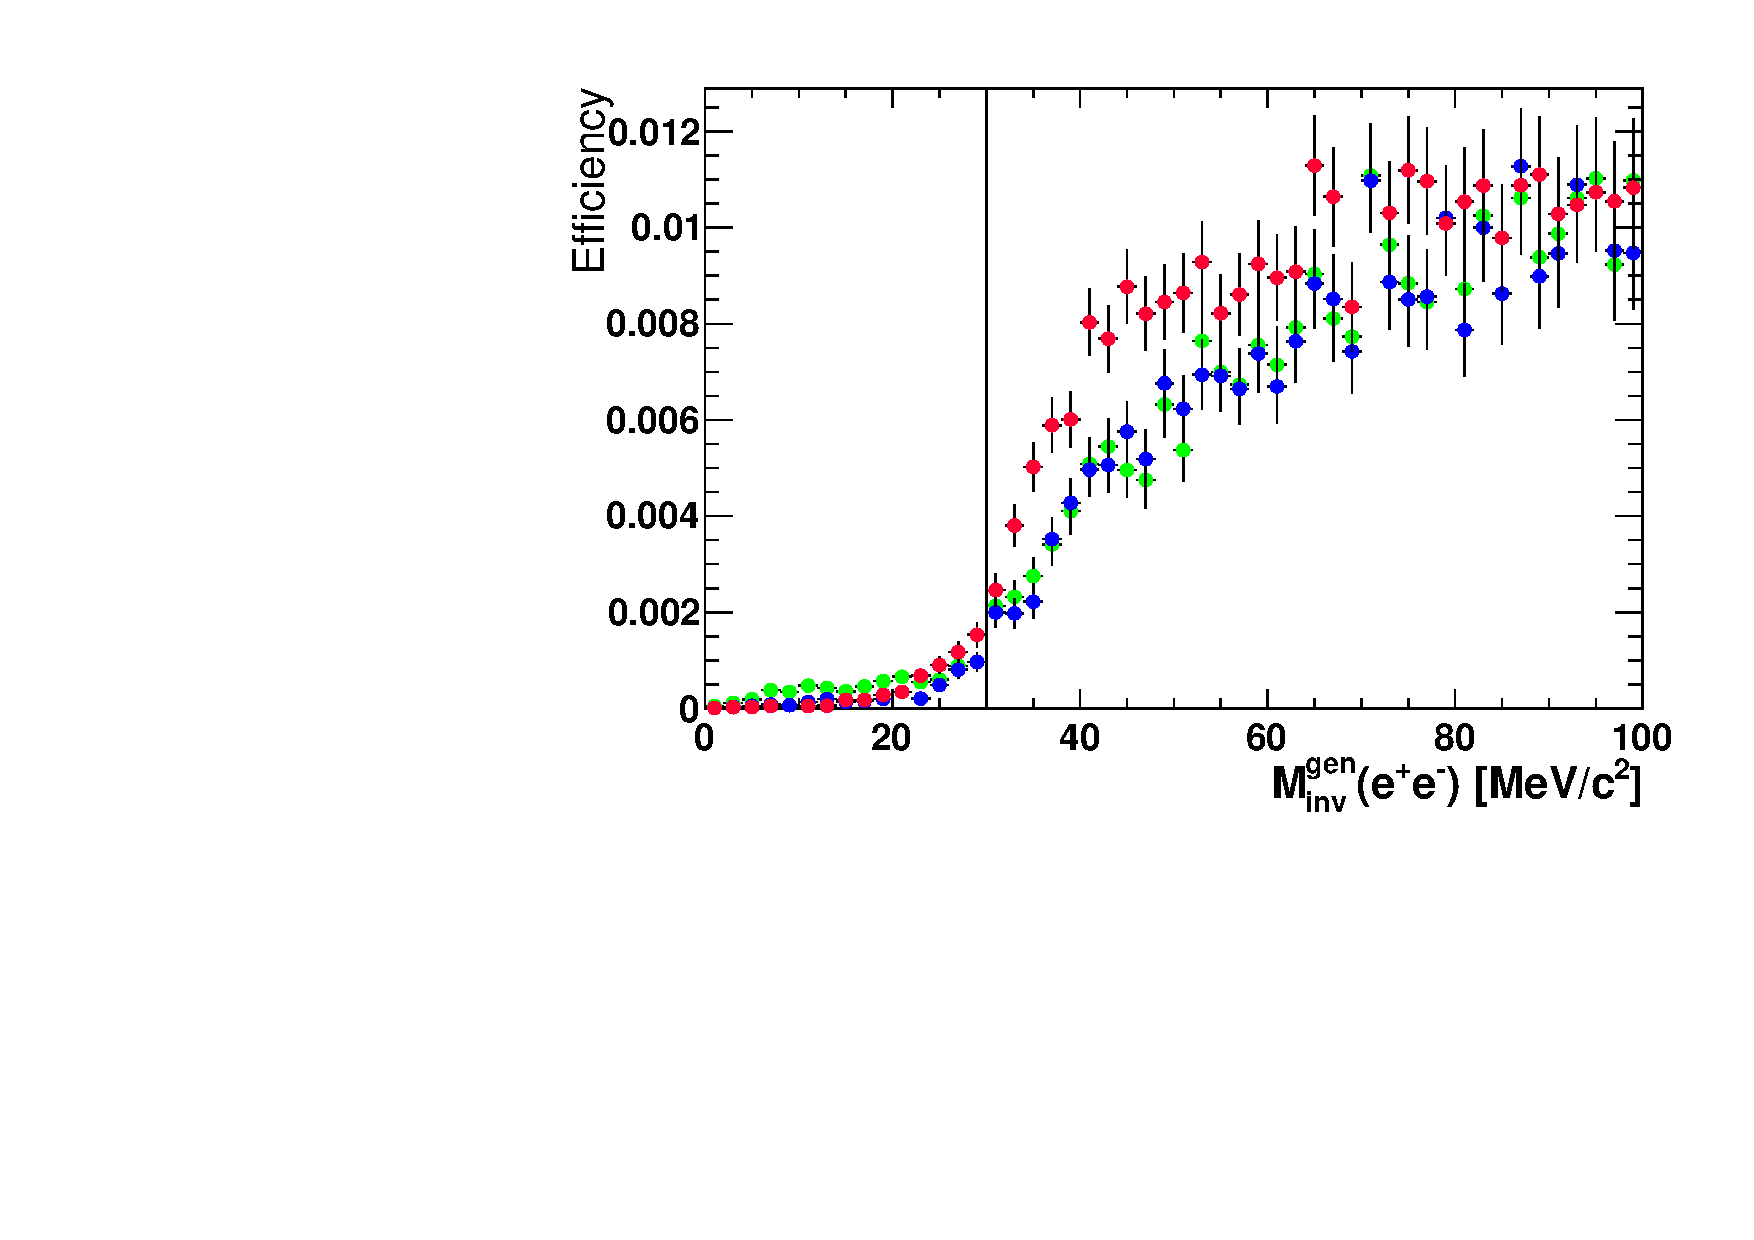
\includegraphics[scale=0.6]{eff_diElectron.pdf}
  \vspace*{-0.5cm}
  \end{center}
  \caption{\textit{Absolute event reconstruction and selection efficiency depending on the generated $M^{gen}_{inv}(\epem)$. Obtained from \BdKstee Monte Carlo by comparing the $M^{gen}_{inv}(\epem)$ at generator level with the $M^{rec}_{inv}(\epem)$ distribution after reconstruction and selection. Green: \davinci v29, blue: \davinci v30, pink: \davinci v30 with \dielectronmaker .}}
  \label{fig:eff_diElectron}
\end{figure}
\vspace*{10cm}


%%%%%%%%%%%%%%%%%%%%%%%%%%%%%%%%%%%%%%%%%%%%%%%%%%%%%%%%%%%%%%%%%%%%%%%%%%%%%%%%%%%%%%%%%%%%%%%%%%%%%%%%%%%%
%Events with double counting were identified by comparing the energy of the Bremsstrahlung photon. If this energy was non zero and the same for the photon coming %from the electron and from the positron within $5 \mev$, the event was considers to be a double counting event.

%To compare the performance of the two n-tuples of \lhcb \BdKstee Monte Carlo are created with the different bremsstrahlung recovery algorithms respectively. Then %the double counting correction is applied to both n-tuples.\\

%\subsection{DaVinci v29r1p1 BremAdder}
%\label{sub:oldBrem}
%As a first step a NTuple was created using DaVinci v29r1p1 and its standard Bremsstrahlung recovery tool. This BremAdder matches photons to the electrons by lineraly extrapolating the
%electron track from its last state before the TT to the calorimeter. If the $\chi_{brem}^2$ of the extrapolated track and the photon position in the calorimeter is less than 300, this photon is
%considerd a bremsphoton and its energy is added to the electron.\\
%Complementing this BremAdder algorithm by the \textit{double counting- correction} yields the $B^0$ mass shape in \ref{fig:oldBremAdder}. The weighted sigma of this shape is $\sigma_{w} = $.\\
%\begin{figure}[ht]
%  \begin{center}
%    \includegraphics[scale=0.6]{figs/Bmass_oldBremdcc.pdf}
%  \vspace*{-1.0cm}
%  \end{center}
%  \caption{$B^0$ mass shape for the DaVinci v29r1p1 bremsstrahlung recovery tool and double- counting correction}
%  \label{fig:oldBremAdder}
%\end{figure}
%
%\subsection{DaVinci v31r0 BremAdder}
%\label{sub:newBremAdder}
%For the second procedure a NTuple was created using DaVinci v31r0 and its standard Bremsstrahlung recovery tool. This new BremAdder is an enhanced version of the BremAdder in \ref{sub:oldBrem}. It
%uses the StdAllLoosePhotons as bremsphoton candidates by default. A photon is matched as a bremsphoton if:
%\begin{itemize}
% \item its X- position in the calorimeter is between the extrapolated X- position of the electrons first state and its extrapolated X- position from the TT within $n_x \cdot \sigma_x$ (default:
%$n_x = 2$, $\sigma_x =$ quadratic sum of photon cluster spread and track extrapolation uncertainty)
%\item its Y- position in the calorimeter matches the extrapolated Y- position from the TT within $n_y \cdot \sigma_y$ (default: $n_y = 2$, $\sigma_y =$ quadratic sum of photon
%cluster spread and track extrapolation uncertainty).
%\end{itemize}
%Complementing this BremAdder algorithm by the \textit{double counting- correction} yields the $B^0$ mass shape in \ref{fig:newBremAdder}. The weighted sigma of this shape is $\sigma_{w} = $.\\
%\begin{figure}[ht]
%  \begin{center}
%    \includegraphics[scale=0.6]{figs/Bmass_newBremdcc.pdf}
%  \vspace*{-1.0cm}
%  \end{center}
%  \caption{$B^0$ mass shape for the DaVinci v31r0 bremsstrahlung recovery tool and double- counting correction}
%  \label{fig:newBremAdder}
%\end{figure}
%
%
%\subsection{DaVinci v32 DiElectronMaker}
%\label{sub:DiElectronMaker}
%For the DaVinci v31r0 a new tool to make $e^+ e^-$ pairs has been developed (also configurable to find same sign pairs). This Tool - called \textit{DiElectronMaker} - takes the electron ProtoParticles
%and creates low invariant mass $e^+ e^-$ pairs. The DiElectronMaker uses a method of the new BremAdder (from the DaVinci v31r0) which makes it possible to avoid the double counting. In the
%case of one bremsphoton candidate matching both electrons this method adds the bremsphoton to one randomly chosen electron - 
%The DiElectronMaker then selects $e^+ e^-$ pairs that pass
%
%
%
%
%\begin{figure}[ht]
%  \begin{center}
%    \includegraphics[scale=0.6]{figs/Bmass_diElectron.pdf}
%  \vspace*{-1.0cm}
%  \end{center}
%  \caption{$B^0$ mass shape for the DaVinci v31r0 DiElectronMaker}
%  \label{fig:diElectronMaker}
%\end{figure}
%\section{Effect of bremsstrahlung radiation on the \Bd mass shape}
%The emittance of bremsstrahlung photons has two different effects on the reconstructed \Bd mass shape.\\
%The first effect can be seen on the Monte Carlo sample in Figure \ref{fig:noBremReco}. If the bremsstrahlung photons are not recuperated the measured electron energy will be smaller than the initial electron energy $E^{measured}_{\epm} = (1 - E_{bs}) E^0_{\epm}$ and this offset will propagate to the reconstructed \Bd mass. Figure \ref{fig:noBremReco} shows the \Bd mass distribution obtained without any bremsstrahlung reconstruction. The distribution has an asymmetric, non Gaussian shape with a very large radiative tail in the low \Bd mass region. Since this tail diminishes the resolution on the \Bd mass and even exceeds the reconstructed mass region, it is crucial to recuperate the emitted bremsstrahlung photons and associate them to their electrons.\\
%This bremsstrahlung recovery causes the second effect on the measured \Bd mass distribution.
%In \lhcb the energy measurement of charged particle is performed by using combined information from the tracking system and the particle identification system. The tracking system determines the momentum of the charged particle $p_T^{track}(c.p.)$ with an accuracy of about $0.5 /$\%. The particle identification system determines the identity of the particle which fixes the invariant mass of the particle track to the PDG value $m_{PDG}(c.p.)$. The particle's energy is then calculated from the combination of the measured momentum and the PDG mass $E(c.p.) = \sqrt{p^2_{track}(c.p.) + m_{PDG}(c.p.)}$. This allows for an energy resolution of the order of the momentum resolution for charged particles.\\
%For neutral particles however, the energy measurement has to be performed by the calorimeter. Since the energy resolution of the calorimeter is much worse than the momentum resolution obtained by the tracking system, the energy resolution of neutral particles is much worse than the energy resolution of charged particles.\\
%Electrons, like muons, are charged particles and their tracks' transverse momenta $p_T^{track}(\epm)$ could be determined with an accuracy up to $0.35$\%. The energy of the bremsstrahlung photons however, has to be determined by the \ecal. The increase in uncertainty on the electron energy will be propagate to the measured \Bd mass. In particular, the \Bd mass distribution reconstructed from \BdKstee will show a greater width than the \Bd mass distribution reconstructed from \BdKstmumu for example.
%Figure \ref{fig:electronAndMuonBMass} shows the comparison between the \Bd mass shape of the \BdKstee and the \BdKstmumu.
%\begin{figure}[ht]
%  \begin{center}
%  \subfigure{
%  	\label{fig:eeKstar}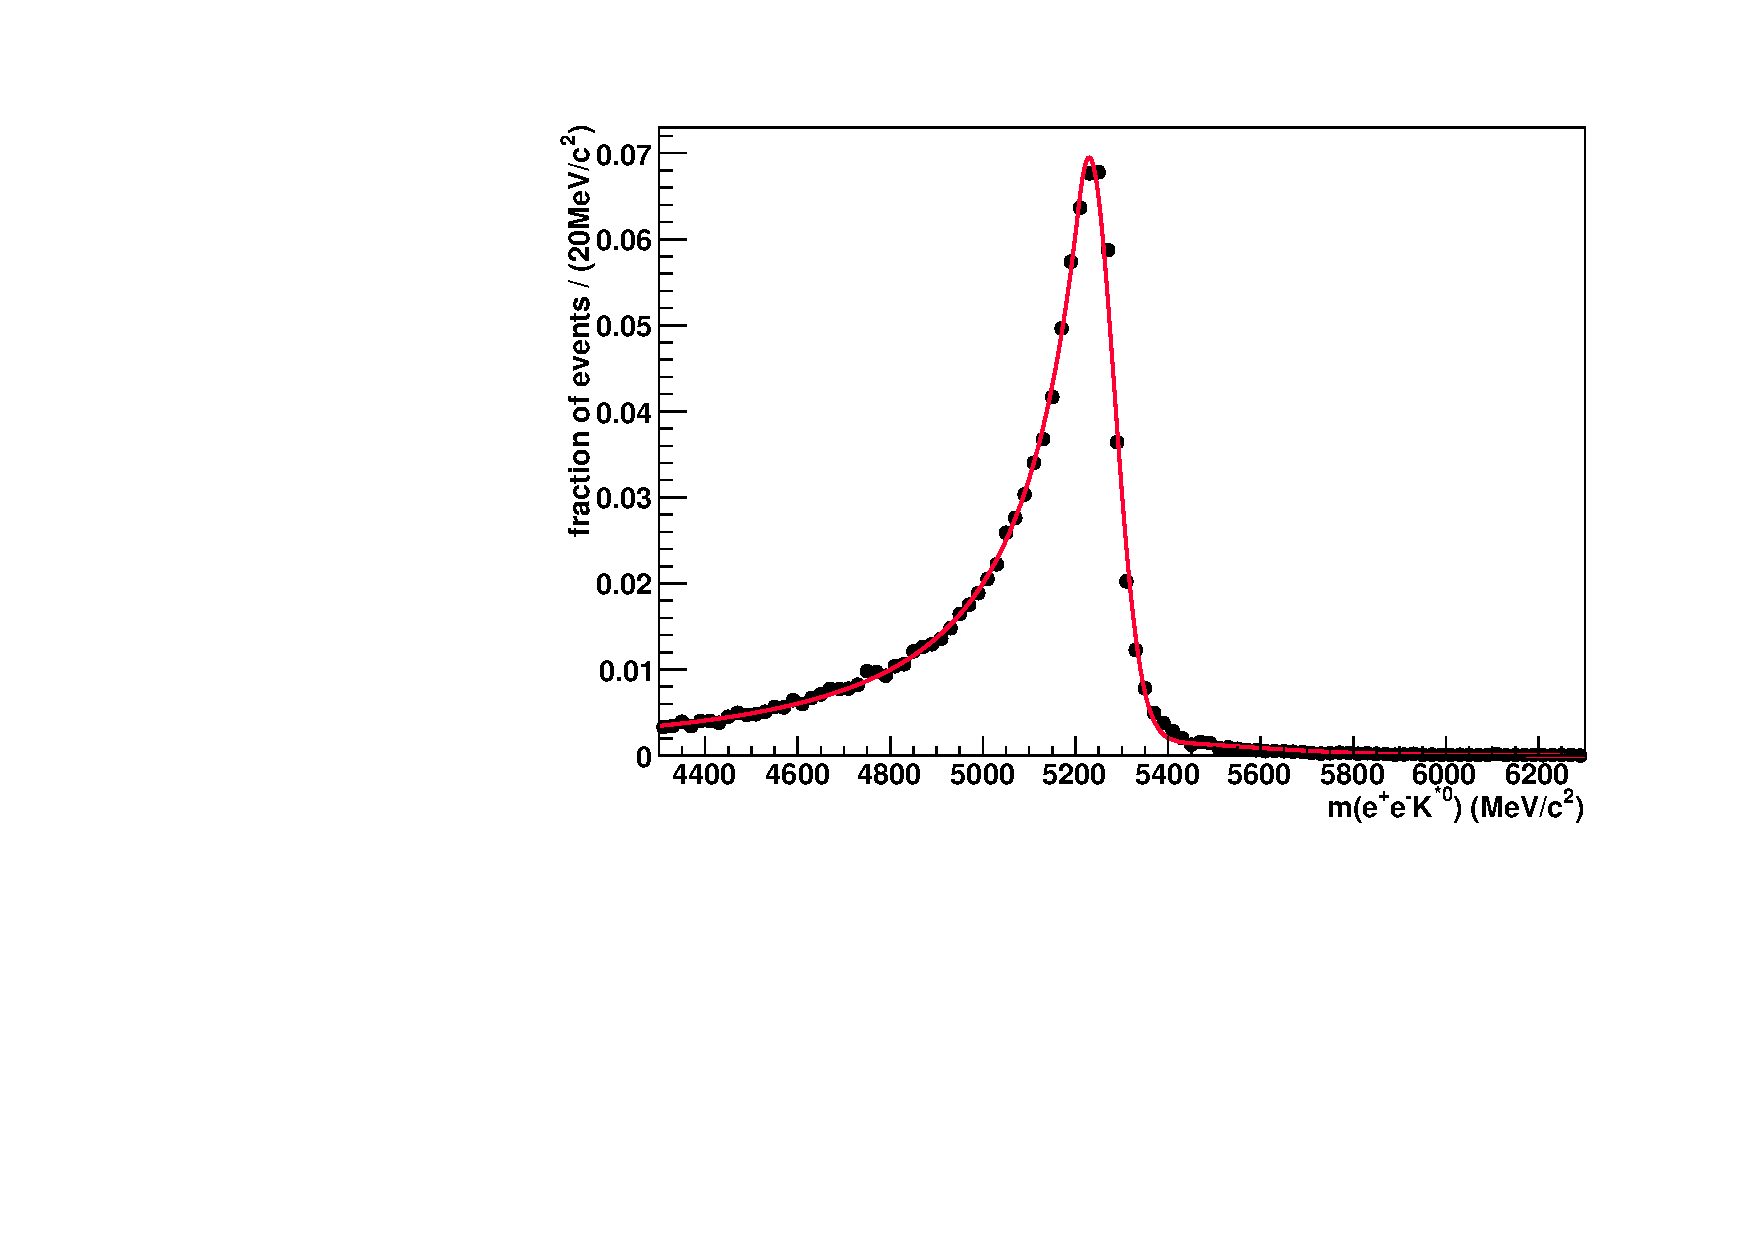
\includegraphics[width=0.49\textwidth]{MC_Bmass_dielectron_TM.pdf}}
%  \subfigure{\label{fig:mumuKstar}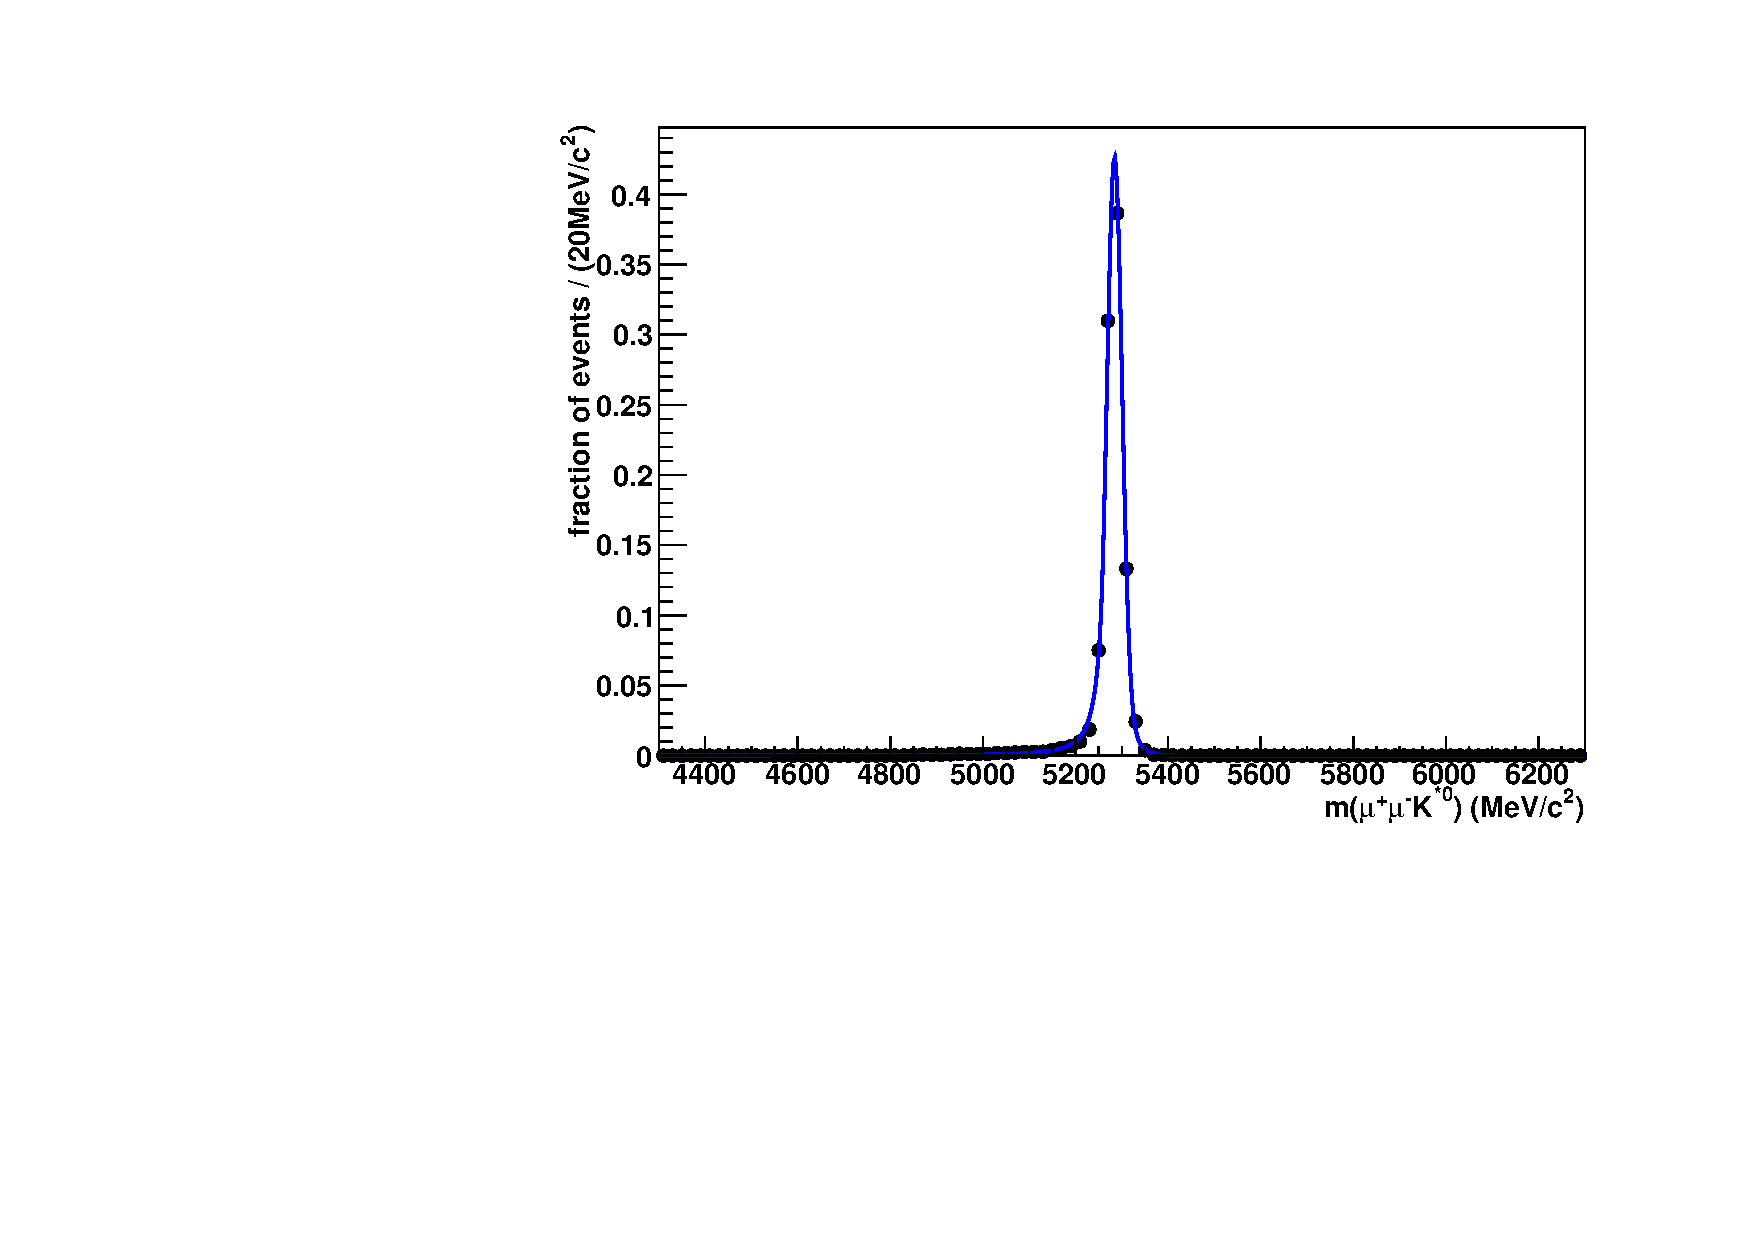
\includegraphics[width=0.49\textwidth]{MC_Bmass_mumuKstar_TM.pdf}} 
%  \vspace*{-1.0cm}
%  \end{center}
%  \caption{\textit{Comparison of the \Bd mass distribution from \BdKstee (left) and \BdKstmumu (right) reconstructed from \lhcb Monte Carlo samples.}}
%  \label{fig:electronAndMuonBMass}
%\end{figure}



 



\end{document}
%% end of file
